\documentclass[a4paper, twoside]{report}
\usepackage[table,x11names]{xcolor}
\usepackage[top=2.5cm,bottom=2.5cm,left=3.0cm,right=2.0cm]{geometry}
\usepackage{fancybox}
\usepackage[utf8]{}
\usepackage[utf8]{inputenc}
\usepackage[vietnamese,main=english]{babel}
\usepackage{multicol}
\usepackage{tabularx}
\usepackage{xcolor, color, soul}
%\usepackage{indentfirst}
\usepackage{float}
\usepackage{enumitem}
\usepackage[nottoc]{tocbibind}
\usepackage{afterpage}
\usepackage[super]{nth}
\usepackage{titlesec}
\usepackage{bigdelim}
\usepackage[titles]{tocloft}
\usepackage{makecell}
\usepackage{arydshln}
\usepackage{url}
\usepackage{perpage} %the perpage package
\usepackage{caption}
\usepackage{listings}
\usepackage{pdfpages}
\usepackage{lstautogobble}
\usepackage{gensymb}
\usepackage{siunitx}
\usepackage{tikz}
\usepackage{mathrsfs}
\usepackage{minted}
\usepackage[american voltages, american current]{circuitikz}
\usepackage{pgfplots}
\usepackage{cancel}
\usepackage{xurl}
\usepackage[bottom]{footmisc}
\usepackage[font=footnotesize,labelfont={scriptsize}]{subfig}
\usepackage{wrapfig}
\usepackage{latexsym,amssymb,amsmath}
%\usepackage{algpseudocode}
\usepackage{pdflscape}
\usepackage{tocvsec2}
\usepackage{fancyref}
\usepackage{bookmark}
\usepackage{hyperref}
\usepackage[nameinlink,noabbrev]{cleveref}
\usepackage{everypage}
\usepackage[parfill]{parskip}
\usepackage[style=ext-numeric, sorting=none, backend=biber, alldates=terse,]{biblatex}
\usepackage{epstopdf}
\usepackage{chngcntr}
\counterwithout{figure}{chapter}
\counterwithout{table}{chapter}
\usepackage{xparse}% http://ctan.org/pkg/xparse

\addbibresource{main.bib}

\nocite{*}

\usemintedstyle{tango}


\setminted{fontsize=\fontsize{11pt}{11pt}, frame=single, linenos, xleftmargin=20pt, breaklines}
\setmintedinline{fontsize=\fontsize{13pt}{13pt}}
\renewcommand\theFancyVerbLine{\normalsize\arabic{FancyVerbLine}}

\newenvironment{code}{\captionsetup{type=listing}}{}

% FLOW CHART
\tikzstyle{startstop} = [rectangle, rounded corners, minimum width=3cm, minimum height=1cm,text centered, draw=black, fill=red!30]
\tikzstyle{io} = [trapezium, trapezium left angle=70, trapezium right angle=110, minimum width=3cm, minimum height=1cm, text centered, draw=black, fill=blue!30]
\tikzstyle{process} = [rectangle, minimum width=3cm, minimum height=1cm, text centered, draw=black, fill=orange!30, text width=4cm]
\tikzstyle{decision} = [diamond, aspect=2.5, minimum width=3cm, minimum height=1cm, text centered, draw=black, fill=green!30]
\tikzstyle{arrow} = [thick,->,>=stealth]

\usetikzlibrary{shapes,positioning,arrows,calc,automata, positioning, arrows,matrix}

\newcolumntype{Y}{>{\centering\arraybackslash}X}

\PassOptionsToPackage{hyphens}{url}

\newcommand\blfootnote[1]{%
  \begingroup
  \renewcommand\thefootnote{}\footnote{#1}%
  \addtocounter{footnote}{-1}%
  \endgroup
}

\newcommand{\Lpagenumber}{\ifdim\textwidth=\linewidth\else\bgroup
  \dimendef\margin=0 %use \margin instead of \dimen0
  \ifodd\value{page}\margin=\oddsidemargin
  \else\margin=\evensidemargin
  \fi
  \raisebox{\dimexpr -\topmargin-\headheight-\headsep-0.5\linewidth}[0pt][0pt]{%
    \rlap{\hspace{\dimexpr \margin+\textheight+\footskip}%
    \llap{\rotatebox{90}{\thepage}}}}%
\egroup\fi}
\AddEverypageHook{\Lpagenumber}%

% \hypersetup{
% 	hidelinks,
%     linktoc=all,
%     bookmarks=true,
% }
\captionsetup[subfloat]{labelformat=empty}

\makeatletter
\pgfcircdeclarebipole{}{\ctikzvalof{bipoles/vsourceam/height}}{vsourceAM}{\ctikzvalof{bipoles/vsourceam/height}}{\ctikzvalof{bipoles/vsourceam/width}}{%
  \pgfsetlinewidth{\pgfkeysvalueof{/tikz/circuitikz/bipoles/thickness}\pgfstartlinewidth}
   \pgfpathellipse{\pgfpointorigin}{\pgfpoint{0}{\pgf@circ@res@up}}{\pgfpoint{\pgf@circ@res@left}{0}}
   \pgfusepath{draw}
   \pgfscope
       \pgftransformxshift{0.6*\ctikzvalof{bipoles/vsourceam/margin}\pgf@circ@res@left}
       \pgftext[rotate=-\pgf@circ@direction]{$+$}
       \pgfusepath{draw}
   \endpgfscope
   \pgfscope
       \pgftransformxshift{0.6*\ctikzvalof{bipoles/vsourceam/margin}\pgf@circ@res@right}
       \pgftext[rotate=-\pgf@circ@direction]{$-$}
       \pgfusepath{draw}
   \endpgfscope
}
\makeatother

\MakePerPage{footnote} %the perpage package command
\usetikzlibrary{shapes,positioning,arrows,calc}

\newcommand*\justify{%
  \fontdimen2\font=0.4em% interword space
  \fontdimen3\font=0.2em% interword stretch
  \fontdimen4\font=0.1em% interword shrink
  \fontdimen7\font=0.1em% extra space
  \hyphenchar\font=`\-% allowing hyphenation
}
\renewcommand\cftchapafterpnum{\vskip-2pt}
\renewcommand\cftsecafterpnum{\vskip-2pt}

\renewcommand{\theequation}{\arabic{equation}}

% FLOW CHART
\tikzstyle{startstop} = [rectangle, rounded corners, minimum width=3cm, minimum height=1cm,text centered, draw=black, fill=red!30]
\tikzstyle{io} = [trapezium, trapezium left angle=70, trapezium right angle=110, minimum width=3cm, minimum height=1cm, text centered, draw=black, fill=blue!30]
\tikzstyle{process} = [rectangle, minimum width=3cm, minimum height=1cm, text centered, draw=black, fill=orange!30, text width=4cm]
\tikzstyle{decision} = [diamond, aspect=2.5, minimum width=3cm, minimum height=1cm, text centered, draw=black, fill=green!30]
\tikzstyle{arrow} = [thick,->,>=stealth]

% CHAPTER FORMAT
\titleformat{\chapter}%[display]
{\bfseries\fontsize{25}{30}\selectfont\raggedright}% Format and size of title text
{\llap{%
    \rule[-6pt]{6cm}{1.1cm}\rule{6pt}{0pt}}% Black box to the left, lowered 6pt. The end rule is a horisontal space.
  \llap{% Number also to the left, on top of the black box.
    \fontsize{25}{37}\selectfont\color{white}\thechapter\rule{9pt}{0pt}}}{0pt}{}{}

%\counterwithin{figure}{chapter}
%\renewcommand{\thefigure}{\arabic{chapter}.\arabic{section}.\alph{figure}}

\renewcommand{\thetable}{\arabic{table}}

\renewcommand\labelitemi{$-$}

\newcommand{\comment}[1]{}
  
\titleformat{\section}
  {\LARGE\bfseries}{}{}{}
\renewcommand\thesection{\arabic{section}.}
\renewcommand\thesubsection{\arabic{subsection}}
\makeatletter
\renewcommand*\l@section{\@dottedtocline{1}{1.5cm}{2em}}
\renewcommand\section{\@startsection {section}{1}{-1em}%
  {-3.5ex \@plus -1ex \@minus -.2ex}%
  {2.3ex \@plus.2ex}%
  {\normalfont\Large\bfseries}}
\def\sectionmark#1{%
      \markright {\MakeUppercase{#1}}}
\makeatother

\titleformat{\subsection}
  {\normalfont\bfseries}{\thesubsection.}{0.5em}{}
\renewcommand\cftsubsecaftersnum{.} 
\renewcommand\thesubsection{\alph{subsection}}

\addto{\captionsenglish}{%
  \renewcommand{\bibname}{References}
}

\setcounter{tocdepth}{1}
%\addtocontents{toc}{\setcounter{tocdepth}{2}}
%\addtocontents{lof}{\vskip -1.6cm}
%\addtocontents{lot}{\vskip -1.6cm}

\newcolumntype{c}[1]{>{\centering\arraybackslash\hspace{0pt}}p{#1}}
    
% TOC settings
\renewcommand\cftchapnumwidth{2.8em}
\renewcommand\cftsecnumwidth{3em}
\renewcommand\cftsecindent{3em}
\renewcommand\cftsubsecindent{5em}
\renewcommand\thechapter{\Roman{chapter}}
    
%\titleformat{\chapter}[display]{\normalfont\huge\bfseries}{}{0pt}{\Huge}
\newcommand{\hsp}{\hspace{20pt}}
%\titleformat{\chapter}[hang]{\Huge\bfseries}{\thechapter\hsp\textcolor{gray75}{|}\hsp}{0pt}{\Huge\bfseries}
\titleformat*{\subsubsection}{\large\bfseries}
%\titlespacing*{\chapter}{0pt}{0pt}{0pt}
    
\newcolumntype{P}[1]{>{\centering\arraybackslash}p{#1}}
\newcolumntype{C}{>{\centering\arraybackslash}p{1.5em}}
\newcolumntype{D}{>{\centering\arraybackslash}p{3em}}
    
\setlist[itemize]{noitemsep, topsep=0pt}
%\AtBeginEnvironment{multicols}{\RaggedRight}

\titlespacing*{\chapter}{0pt}{0pt}{20pt}

\newcommand\Chapter[2]{\chapter
  [#1\text{: }\hfil\hbox{}\protect\linebreak{\itshape#2}]%
  {#1\\[-0.75ex]\Large#2}%
  \markboth{\MakeUppercase{\chaptername\ \thechapter.\ #1}}{}%
}


\def\doubleoverline#1{\overline{\overline{#1}}}

\usepackage{graphicx}
\begin{document}
%Trang bìa 1
\fontsize{13pt}{18pt}\selectfont
\begin{titlepage}
%\thispagestyle{empty}
%\thisfancypage{%đóng khung trang này
%\setlength{\fboxsep}{0pt}% 8pt là độ dày của đường viền
%\fbox
%}{} % phần nội dung sau là tương tự như đã làm
%\

\begin{tikzpicture}[remember picture, overlay]
  \draw[line width = 1pt] ($(current page.north west) + (2cm,-2cm)$) rectangle ($(current page.south east) + (-2cm,2cm)$);
\end{tikzpicture}

\begin{center}
\begin{large}
HO CHI MINH CITY UNIVERSITY OF TECHNOLOGY $-$ VNU HCMC
\end{large} \\
\begin{large}
OFFICE FOR INTERNATIONAL STUDY PROGRAM
\end{large} \\
\begin{large}
FACULTY OF ELECTRICAL AND ELECTRONICS ENGINEERING
\end{large} \\
\textbf{--------------------  *  --------------------}\\[1.5cm]

\includegraphics[scale=0.1]{logobk.png}\\[1.5cm]
{\fontsize{19pt}{1}\bfseries \selectfont Embedded System Design}\\[0.2cm]
{\fontsize{21pt}{1}\bfseries\selectfont Scientific Calculator
}\\[3.3cm]
\end{center}

\begin{otherlanguage}{vietnamese}
\begin{tabbing}
	\hspace{2.5cm}Instructors  \ \=: \ \textbf{\parbox[t]{9cm}{M.S. Bùi Quốc Bảo}}\\
	\hspace{2.5cm}Subject \>: \ \textbf{\parbox[t]{12cm}{Embedded System Design}}\\
	\hspace{2.5cm}Class \>: \ \textbf{\parbox[t]{9cm}{TT01}}\\
	\hspace{2.5cm}Members \>: \ \textbf{\parbox[t]{9cm}{
		Lương Triển Thắng - 2051194 }}\\
	\hspace{3.5cm} \>\ \ \ \textbf{\parbox[t]{9cm}{
		Đinh Hoàng Luân - 2051145 }}\\
	\hspace{3.5cm} \>\ \ \ \textbf{\parbox[t]{9cm}{
		Bùi Thanh Tùng - 2051213 }}\\
        \hspace{3.5cm} \>\ \ \ 
\end{tabbing}
\end{otherlanguage}

\vspace{3.8cm}
\begin{center}
{\fontsize{13pt}{1}\selectfont Ho Chi Minh City, \nth{29} May, 2023}
\end{center}
\end{titlepage}

\afterpage{\null\newpage}

\setcounter{page}{0}
\tableofcontents
\listoffigures


\chapter{Abstract}
This project report presents the development of an advanced calculator with user-friendly features. The calculator is designed for easy assembly through soldering and can be connected to smartphones and computers via UART. It incorporates a rechargeable battery and Micro-USB charging port for convenience. The calculator offers basic arithmetic operations, advanced mathematical functions, and supports calculus operations and graphing. Memory functions allow storing and recalling values, while a high level of accuracy is ensured with support for 10 decimal places. The calculator features adjustable screen brightness, a clear interface, and accessibility options. It is cost-effective, lightweight, and portable, with easy maintenance and upgradability. The calculator emphasizes reliability, energy efficiency, and responsiveness, making it suitable for a diverse range of users and applications.

% This project report outlines the development of an easy-to-use and understandable calculator with various advanced features. The calculator is designed to be easily assembled through soldering and can be connected to smartphones and computers via UART). It features a rechargeable battery that can be charged through a Micro-USB port, ensuring convenience for users. The calculator includes an adjustable screen brightness and contrast to enhance visibility.

% Functionally, the calculator supports basic arithmetic operations such as addition, subtraction, multiplication, and division. It also offers advanced mathematical functions like exponentiation, logarithms, trigonometric functions, and calculus operations such as limits, derivatives, and integrals. Additionally, the calculator provides memory functions with three user-defined slots for storing, recalling, and clearing values. The most significant function is that our calculator can graph the functions and return the value of derivative function.

% To facilitate accurate calculations, the calculator supports a minimum of 10 decimal places, catering to scientific and engineering applications. The LCD screen features adjustable back light ensuring readability in various lighting conditions. The calculator has a user-friendly interface with clearly labeled keys and functions, promoting ease of use and understanding.

% Other important aspects of the calculator include cost-effectiveness, lightweight and portable design, easy maintenance and upgradability, energy efficiency, fast and responsive performance, reliability with minimal errors or malfunctions, and user-friendliness. Accessibility features are also incorporated, such as large display font sizes and high contrast mode, making it accessible to users with disabilities.

% To ensure the calculator's longevity and continued usability, adequate support and maintenance are provided, including regular updates and bug fixes. Overall, this calculator meets the desired requirements and specifications, offering a versatile and reliable tool for a wide range of users in various situations and environments.

\chapter{Introduction}
\section{Introduce the problem}
A scientific calculator is a type of calculator designed to perform complex mathematical operations. It can perform logarithmic, trigonometric, statistical and other advanced functions that are not typically found on basic calculators. Scientific calculators are commonly used by students, scientists, engineers, and other professionals who need to make precise calculations in their work or studies. They often have more buttons and functions than basic calculators, and can display results with high precision. Many scientific calculators also have features such as memory storage, equation solving, and graphing capabilities.

Scientific calculators are essential tools used in various fields such as engineering and science. These calculators are designed to perform complex mathematical calculations and provide accurate results. With the advancements in technology, it has become possible to design scientific calculators with more advanced features and functionalities. Microcontrollers, in particular, have become a popular choice for calculator designers due to their low power consumption and ability to perform complex tasks.

Here are some calculators available on the market that have similar capabilities to the project's aim:
\begin{itemize}
    \item Texas Instruments TI-84 Plus CE: This graphing calculator offers a wide range of advanced mathematical functions, including calculus operations, trigonometric functions, logarithms, and graphing capabilities. It has a user-friendly interface, a high-resolution color screen, and supports programming.
    \item Casio FX-991EX: This scientific calculator features a large display, supports complex number calculations, matrix operations, vector calculations, and various mathematical functions. It also includes a spreadsheet function, equation solver, and statistical analysis capabilities.
    \item HP 50g: This graphing calculator provides advanced mathematical functions, including calculus, complex numbers, matrix operations, and symbolic algebra. It has a large screen, supports RPN (Reverse Polish Notation), and offers extensive programmability.
    \item Sharp EL-W516TBSL: This scientific calculator supports advanced functions such as complex numbers, calculus, and statistical calculations. It has a large display, supports multi-line input and output, and includes a table function for organizing data.
    \item Casio fx-115ES PLUS: This scientific calculator offers a wide range of mathematical functions, including complex numbers, calculus, and statistical calculations. It has a natural textbook display, supports equation solving, and allows for multi-line input and output.
\end{itemize}

Calculators with similar capabilities can vary in price range. Graphing calculators, offering advanced functionalities and graphing capabilities, typically fall within the range of \$100 to \$200 or more. On the other hand, scientific calculators, providing a wide range of mathematical functions, tend to be more affordable with prices ranging from \$15 to \$100. It's important to consider factors like brand, features, and display quality when determining the specific price within these ranges.

Our device aims to be cost-effective and budget-friendly, with an estimated price of \$25. Compared to other calculators on the market with similar capabilities, which can range from \$15 to \$200, our device offers a competitive and affordable option for users. By leveraging efficient design and cost-effective components, we strive to provide a reliable and feature-rich scientific calculator at a significantly lower price point, making it accessible to a wide range of users.

The aim of this project is to design a comprehensive scientific calculator, utilizing the STM32 microcontroller unit (MCU), that encompasses both hardware and software components. The project aims to create a fully functional calculator with advanced mathematical functions, memory capabilities, a user-friendly interface, and a compact form factor. By leveraging the power and versatility of the STM32 MCU, the goal is to develop a reliable and efficient calculator that meets the diverse needs of users in scientific, engineering, and mathematical fields. The project will involve the design of the calculator's PCB, 3D-printed case, and the development of firmware to implement the necessary mathematical operations, user interface, and memory management.

\section{Objectives}
Design a complete system, including hardware and software:
\begin{itemize}
    \item Design and develop a Printed Circuit Board (PCB) that accommodates the necessary components and facilitates easy soldering, ensuring a reliable and efficient hardware design.
    \item Create a compact and lightweight 3D-printed case that provides a protective and portable housing for the calculator, allowing for easy use in various environments and situations.
    \item Develop firmware that implements the necessary mathematical functions, including basic arithmetic operations, advanced functions, calculus operations, and graphing capabilities.
\end{itemize}

\begin{figure}[H]
    \centering
    \subfloat[][TI-84 Plus CE (\$125)]{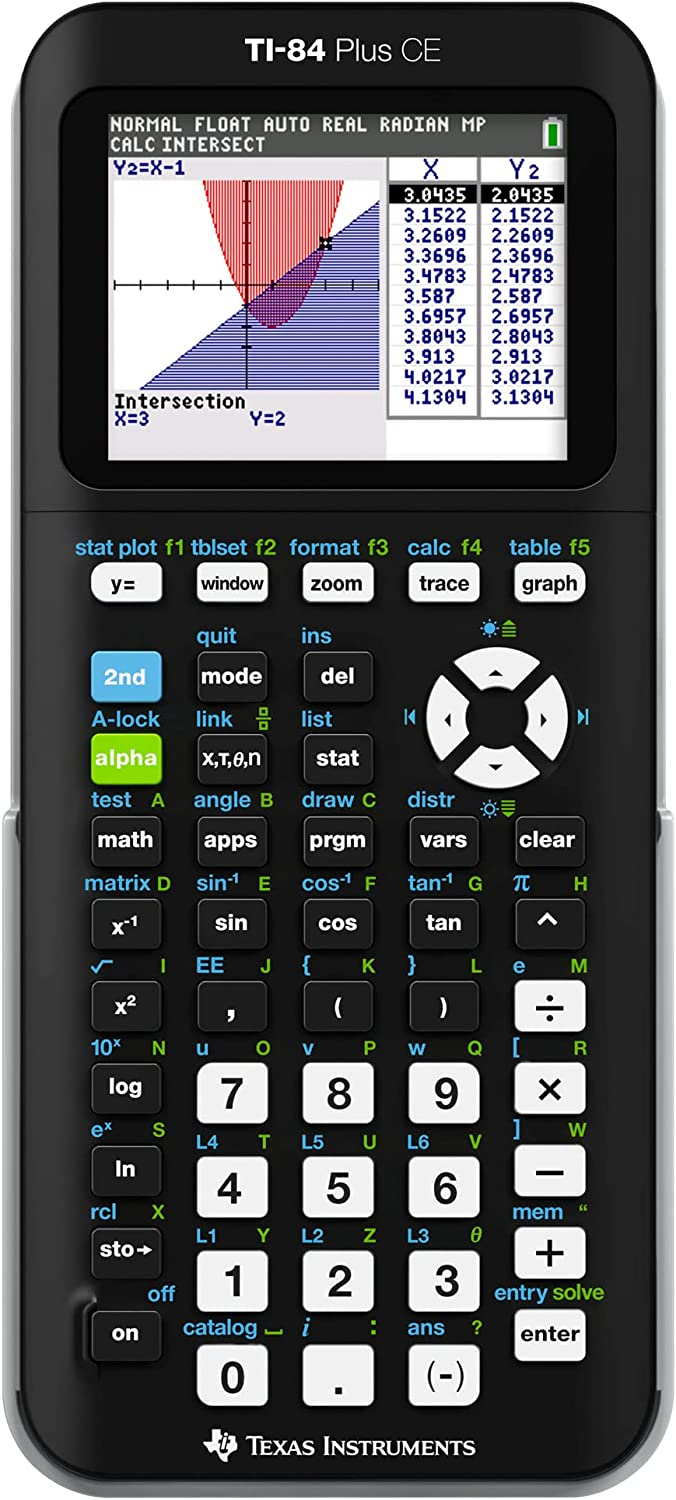
\includegraphics[height=.4\textheight]{images/ti84.jpg}}\qquad\qquad\qquad\qquad\qquad
    \subfloat[][HP 50g (\$250)]{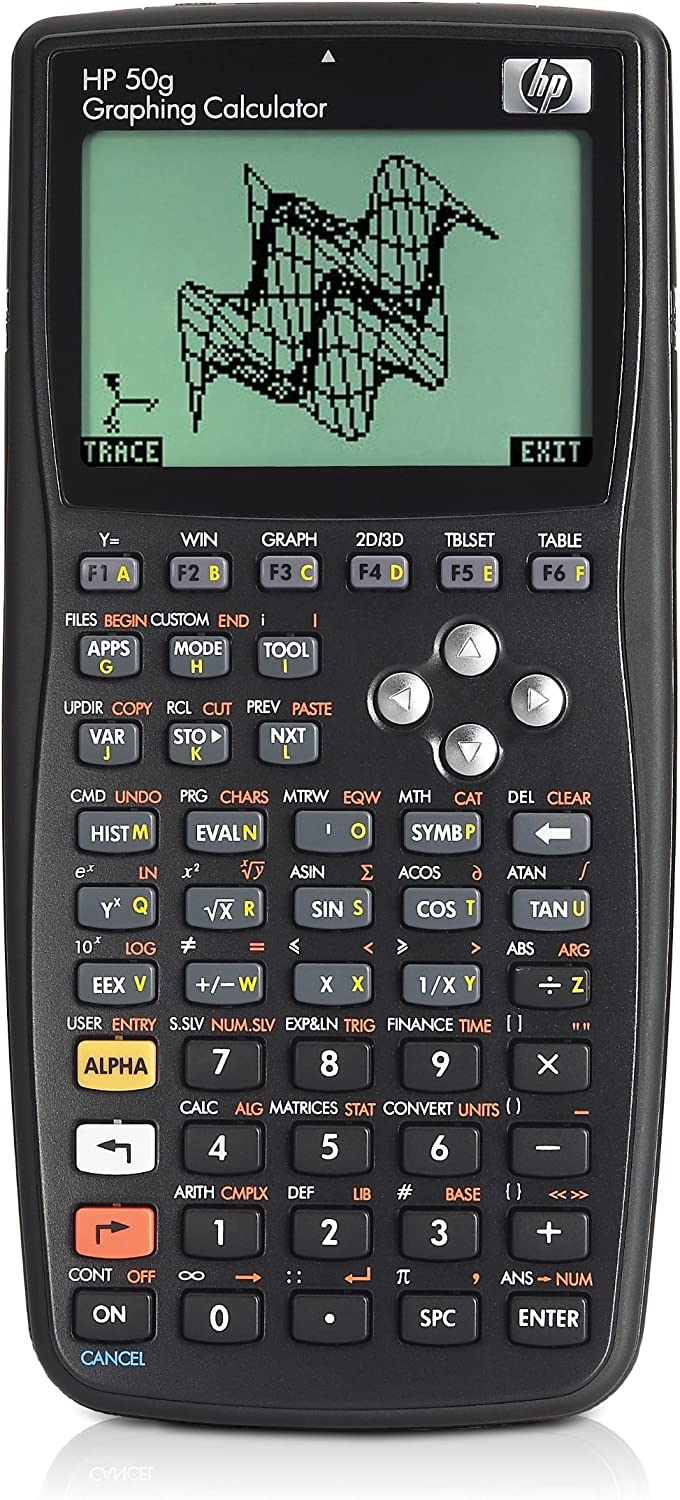
\includegraphics[height=.4\textheight]{images/hp50g.jpg}}
    \caption{Graphing Calculators on the market}
\end{figure}

\section{Requirements}
\subsection{Functional Requirements}
\begin{table}[H]
\centering
\begin{tabular}{|c{.05\textwidth}|p{.6\textwidth}|c{.1\textwidth}|c{.1\textwidth}|}
\hline
\textbf{No.} & \textbf{Description} & \textbf{Satisfied} & \textbf{Note} \\ \hline
F1  & The calculator shall be easy to use and understand.                                                                                                                                                                                                                                                                                                                         & Y                     &  \\ \hline
F2  & The calculator shall be able to perform calculations quickly and accurately.                                                                                                                                                                                                                                                                                                & Y                     &  \\ \hline
F3  & The calculator shall be communicated with smartphones/computers via USB or Bluetooth.                                                                                                                                                                                                                                                                                       & Y                     & partial, UART \\ \hline
F4  & The calculator shall be connected to the Internet via Wi-Fi.                                                                                                                                                                                                                                                                                                                & N                     &  \\ \hline
F5  & The calculator shall have a lightweight web browser and able to render basic website (eg. Google, Wikipedia, etc.)                                                                                                                                                                                                                                                          & N                     &  \\ \hline
F6  & The calculator shall be rechargeable through the USB-C port.                                                                                                                                                                                                                                                                                                                & Y                     & Micro-USB \\ \hline
F7  & The calculator screen brightness shall be adjustable.                                                                                                                                                                                                                                                                                                                       & Y                     &  \\ \hline
F8  & The calculator shall have RTC and show date and time on the screen.                                                                                                                                                                                                                                                                                                         & N                     &  \\ \hline
F9  & The calculator shall be able to perform basic arithmetic operations such as addition, subtraction, multiplication, and division. It shall also support more advanced operations such as exponentiation, logarithms, and trigonometric functions and more. & Y          &  \\ \hline
\end{tabular}
\end{table}

\newpage
\begin{table}[H]
\centering
\begin{tabular}{|c{.05\textwidth}|p{.6\textwidth}|c{.1\textwidth}|c{.1\textwidth}|}
\hline
\textbf{No.} & \textbf{Description} & \textbf{Satisfied} & \textbf{Note} \\ \hline
F10 & The calculator shall provide memory functions to allow the user to store, recall and clear values with more than 50 user-defined memory slots.                                                                                                                                                                                                                              & Y                       & 3 for now \\ \hline
F11 & The calculator shall support at least 10 decimal places, to allow for accurate calculations in scientific and engineering applications.                                                                                                                                                                                                                                     & Y                     &  \\ \hline
F12 & The calculator shall be able to switch between different units of angle measurement, such as degrees, radians, and grads.                                                                                                                                                                                                                                                   & N                     &  \\ \hline
F13 & The calculator shall have a clear, easy-to-read display that shows both the numbers being entered and the results of calculations, and status bar for options and time.                                                                                                                                                                                                     & Y                          & Doesn't have status bar \\ \hline
F14 & The calculator shall have a user-friendly interface, with clearly labeled keys and easy-to-understand functions                                                                                                                                                                                                                                                             & Y              &  \\ \hline
F15 & The calculator shall support firmware updating over the air (OTA).                                                                                                                                                                                                                                                                                                          & N                     &  \\ \hline
\end{tabular}
\caption{Functional Requirements}
\end{table}


\subsection{Non-functional Requirements}
\begin{table}[H]
\centering
\begin{tabular}{|c{.05\textwidth}|p{.6\textwidth}|c{.1\textwidth}|c{.1\textwidth}|}
\hline
\textbf{No.} & \textbf{Description} & \textbf{Satisfied} & \textbf{Note} \\ \hline
NF1  & The calculator shall have an LCD screen with adjustable backlight and contrast.                                                                                               & Y &                         \\ \hline
NF2  & The calculator shall be cost-effective.                                                                                                                                       & Y & 600k VND                \\ \hline
NF3  & The calculator shall be small and lightweight, easy use in a variety of locations and situations.                                                                             & Y &                         \\ \hline
NF4  & The calculator shall be secure from unauthorized access.                                                                                                                      & Y & No internet for now     \\ \hline
NF5  & The calculator shall be easy to maintain and upgrade.                                                                                                                         & Y &                         \\ \hline
NF6  & The calculator shall be energy efficient and use minimal power, it shall last at least 1 week.                                                                                & Y &                         \\ \hline
NF7  & The calculator shall be fast and responsive, providing quick calculations with most basic calculations.                                                                       & Y &                         \\ \hline
NF8  & The calculator shall be reliable and consistent, with a low rate of errors or malfunctions.                                                                                   & Y & some bugs with integral \\ \hline
NF9  & The calculator shall be user-friendly and intuitive, with clear labeling and easy-to-use functions. It should also be easy to carry and use on the go.                        & Y &                         \\ \hline
NF10 & The calculator shall be durable and able to withstand everyday wear and tear, including being dropped, scratched, or exposed to harsh conditions.                             & N &                         \\ \hline
NF11 & The calculator shall be accessible to a wide range of users, including those with disabilities, by providing features such as large display font sizes or high contrast mode. & Y &                         \\ \hline
NF12 & The calculator shall include adequate support and maintenance, such as regular updates and bug fixes, to ensure continued performance and usability over time.                & Y &                         \\ \hline
\end{tabular}
\caption{Non-functional Requirements}
\end{table}

\chapter{Hardware}
\section{Graphic LCD 128x64}
The ST7920 driver-based 12864 Graphic LCD screen in green color refers to a type of LCD (liquid crystal display) screen that utilizes the ST7920 driver and displays a monochrome image in green color. This type of screen has a resolution of 128 x 64 pixels. The ST7920 driver is responsible for controlling the display of information on the screen
\begin{figure}[H]
    \begin{center}
    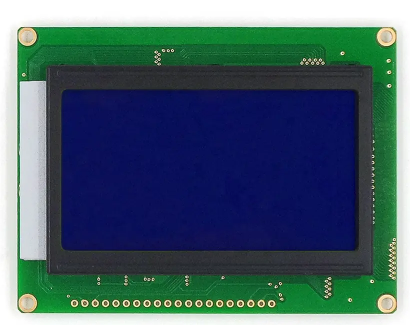
\includegraphics[width=.7\textwidth]{images/LCD.png}
    \caption{STM32F302CCT6 MCU}
    \end{center}
\end{figure} 
For this project, we use the Graphic LCD Monitor 12864 Driver ST7920 Green as it has ST7920 driver supports various display modes, including 8-bit parallel, 4-bit parallel, and serial communication. In addition, the screen's resolution of 128 x 64 pixels and green color display provide great contrast and visibility, making it suitable for displaying text and simple graphics. Furthermore, The LED backlight ensures that the display is easy to read in various lighting conditions. 
\newpage
\section{Power}
\subsection{Lithium Battery}
The Lithium Battery 3.7V 1200mAh PL503759 is a rechargeable lithium-ion battery with a capacity of 1200mAh and a nominal voltage of 3.7 volts. It is a small, lightweight, and high-energy-density battery. This battery is rechargeable and can be charged using a standard lithium-ion battery charger. Typically, the PL503759 battery can be charged in 2-3 hours and can be charged up to 500 times before its capacity begins to degrade.
\begin{figure}[H]
    \begin{center}
    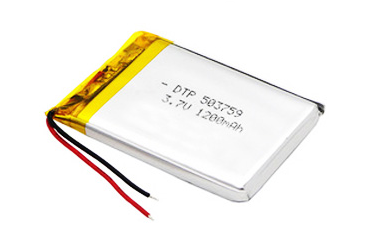
\includegraphics[width=.45\textwidth]{images/Baterry.png}
    \caption{The PL503759 battery}
    \end{center}
\end{figure} 
In this project, our team select the PL503759 battery as it is designed to provide reliable and long-lasting power to electronic devices. It is also equipped with multiple layers of safety protection to prevent overcharging, over-discharging, and short circuits, which can help to extend the lifespan of the battery and ensure safe operation.

\subsection{Charging Circuit}
The TP4056 is a lithium battery charge controller that is commonly used in electronic circuits to charge single-cell lithium-ion or lithium-polymer batteries. It is designed to be connected to a micro USB port or other 5V power source and can charge batteries with a maximum charging current of 1A.
\begin{figure}[H]
    \begin{center}
    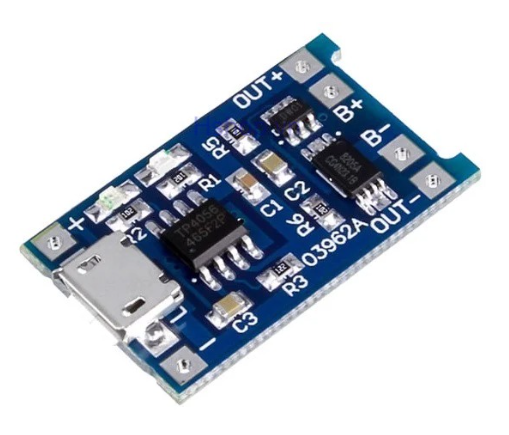
\includegraphics[width=.35\textwidth]{images/TP4056.png}
    \caption{TP4056 Micro USB Lithium Battery Charge Controller}
    \end{center}
\end{figure} 

\subsection{Low-Dropout Regulator}
The LDO SPX3819M5-L-3-3/TR is a low-dropout voltage regulator that is commonly used to regulate voltage in electronic circuits. It is designed to provide a stable and constant output voltage of 3.3 volts with a maximum output current of 0.5 amps. This device achieves voltage regulation by adjusting the resistance of a series pass transistor, which ensures that the output voltage remains constant even as the input voltage changes. The LDO SPX3819M5-L-3-3/TR has a low dropout voltage of 0.5 volts, which means that it can regulate the voltage even when the input voltage is very close to the desired output voltage.
\begin{figure}[H]
    \begin{center}
    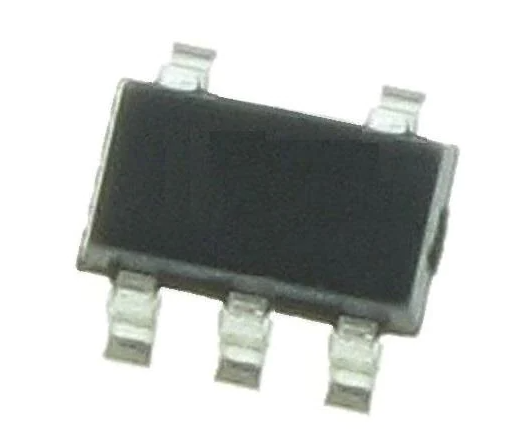
\includegraphics[width=.3\textwidth]{images/LDO.png}
    \caption{The LDO SPX3819M5-L-3-3/TR}
    \end{center}
\end{figure} 
By using the LDO SPX3819M5-L-3-3/TR, it will be used to drop the voltage from 4.2V of the lithium battery to 3.3V in order to adapt to the voltage requirements of the MCU. So we can ensure that the voltage supplied to the MCU is stable and regulated.

\section{Microcontroller}
\subsection{STM32F407 Discovery kit}
The STM32F407 Discovery kit is an evaluation board designed to showcase the capabilities of the STM32F407VG microcontroller. This board is ideal for prototyping and testing applications that require high-performance processing, advanced connectivity, and extensive I/O capabilities. The board is equipped with various features, including USB OTG connectivity, which allows for seamless integration with other systems.

The STM32F407 Discovery kit not only showcases the capabilities of the STM32F407VG microcontroller but also includes a built-in STLink debugger and programmer. This feature allows for seamless programming of other microcontrollers in the STM32 family, adding convenience and flexibility to the development process.

\newpage
\begin{figure}[H]
    \begin{center}
    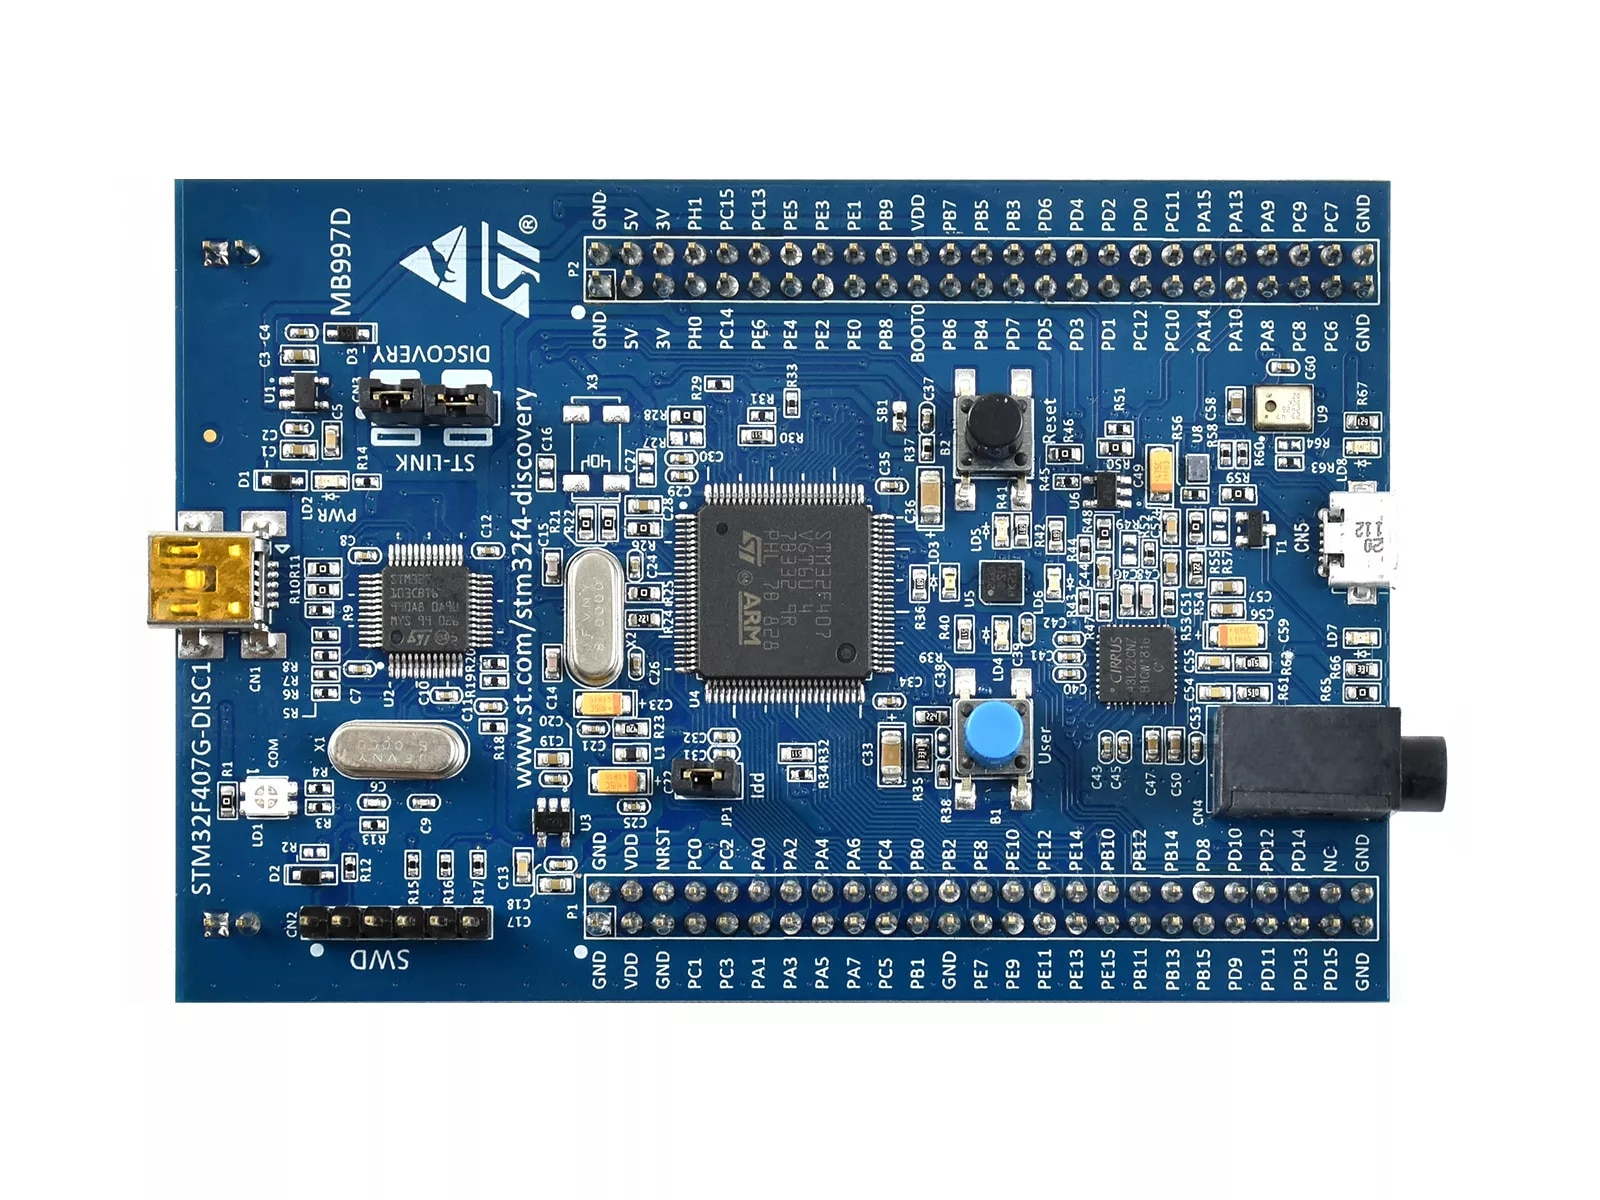
\includegraphics[trim=0cm 6cm 0cm 5cm,clip,width=.6\textwidth]{images/MCU/stm32f4-discovery-3.jpeg}
    \caption{STM32F407 Discovery kit}
    \end{center}
\end{figure} 

In our project, we are using the STM32F407 Discovery kit in the development process. By leveraging the board's advanced processing capabilities and extensive I/O features, we can easily connect the keypad to the board and test its functionality. 

\subsection{STM32F302CCT6 MCU}
The STM32F302CCT6 MCU is a versatile microcontroller unit that is designed for high performance, low power consumption, and advanced analog and digital integration. Based on the ARM Cortex-M4 32-bit RISC core with FPU (Floating Point Unit), these microcontrollers offer advanced processing capabilities with a clock speed of up to 72 MHz. The family includes up to 256 Kbytes of flash memory and up to 40 Kbytes of SRAM, providing ample storage for complex applications. Additionally, The STM32F302CCT6 MCU is housed in a 48-pin LQFP package and operates over a wide temperature range of -40°C to 85°C. With its low-power modes, it is suitable for use in battery-powered applications.

The FPU is an important feature of the STM32F302CCT6 MCU as it allows for high-precision floating-point calculations, which are essential for many advanced applications such as signal processing, control systems, and scientific computing. With the FPU, the MCU can perform complex calculations quickly and accurately, allowing for faster and more efficient processing of data.

\begin{figure}[H]
    \begin{center}
    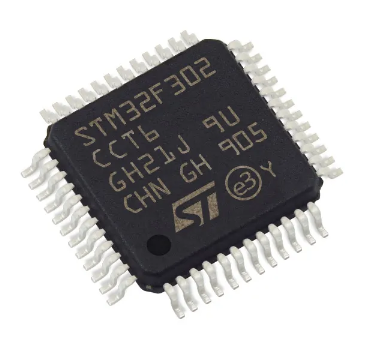
\includegraphics[width=.25\textwidth]{images/MCU/STM32F302CCT6.png}
    \caption{STM32F302CCT6 MCU}
    \end{center}
\end{figure} 
The selection of the STM32F302CCT6 MCU for our project, including its FPU and communication UART. These features allow for high-precision calculations and seamless communication with devices, making the MCU well-suited for a wide range of applications that require advanced processing and communication capabilities.

\section{Other components}
\subsection{SMD LED}
LED SMD is a type of LED that is designed to be mounted directly onto a printed circuit board (PCB) using surface mount technology (SMT). Additionally, SMD LEDs are available in a wide range of sizes, ranging from 0402 (0.4 mm x 0.2 mm) to 5050 (5.0 mm x 5.0 mm). They are also available in a range of colors, including red, green, blue, yellow, and white.
\begin{figure}[H]
    \begin{center}
    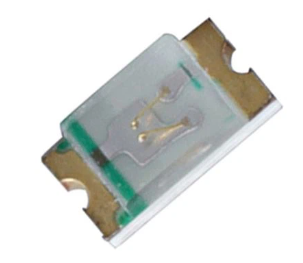
\includegraphics[width=.25\textwidth]{images/LED_Green.png}
    \caption{SMD LED}
    \end{center}
\end{figure} 
In your project, we have chosen to use 0805 LED Green and 0805 LED Red. For the LED Red is primarily used as an indicator light for the power source. It is a commonly used color for indicating the presence of power and can easily be seen in various lighting conditions. On the other hand, the LED Green is connected to the GPIO port of the MCU. This allows for customization of the LED, making it possible to program the MCU to control the LED in different ways.

\subsection{SMD Crystal}
The 32MHz SMD Crystal is a type of oscillator that is used in electronic devices to generate a precise clock signal. Oscillators are used to generate clock signals for microcontroller, digital signal processors, and other electronic devices that require precise timing.
\begin{figure}[H]
    \begin{center}
    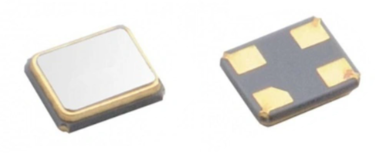
\includegraphics[width=.5\textwidth]{images/crystal.png}
    \caption{SMD Crystal}
    \end{center} 
\end{figure} 
For this project, the crystal SMD (Surface-Mount Device) 32MHz is chosen, which reduces assembly time and allows for high-density placement of components on the PCB. The small size of the SMD package also makes it ideal for use in small and compact electronic devices.

\subsection{SMD Resistor}
Resistor SMD (Surface-Mount Device) is a type of resistor that is designed to be mounted directly onto a printed circuit board (PCB) using surface mount technology (SMT).SMD resistors are available in a wide range of sizes, ranging from 0201 (0.6 mm x 0.3 mm) to 2512 (6.4 mm x 3.2 mm). They are also available in a range of resistance values and tolerances. SMD resistors also offer high accuracy and stability.

\begin{figure}[H]
    \begin{center}
    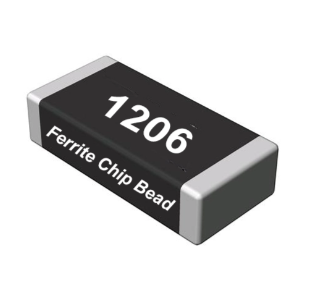
\includegraphics[trim=0cm 1cm 0cm 1cm,clip,width=.25\textwidth]{images/Resistor.png}
    \caption{SMD Resistor}
    \end{center} 
\end{figure} 
 
In this project, we use $330 \si{\ohm}$ and $0 \si\ohm$ 1206 SMD resistors. The 1206 SMD resistors have larger size and ease of handling for hand soldering purposes. The $330 \si\ohm$ SMD resistor is used to protect the LEDs from damage by limiting the current flowing through it, while the $0 \si\ohm$ SMD resistor is used as a short to connect two terminals.

\subsection{SMD Capacitor}
A capacitor SMD (Surface-Mount Device) is a type of capacitor that is designed to be mounted directly onto a printed circuit board (PCB) using surface mount technology (SMT). Additionally, the SMD capacitors are available in a wide range of sizes and capacitance values, and are suitable for a variety of applications, including power supply filtering, decoupling, and timing circuits.  The SMD package of these capacitors allows for easy mounting onto the PCB using SMT techniques, which reduces assembly time and allows for high-density placement of components on the PCB.
\begin{figure}[H]
    \begin{center}
    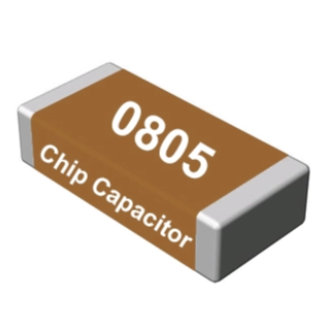
\includegraphics[trim=0cm 1cm 0cm 1cm,clip,width=.25\textwidth]{images/capacitor.png}
    \caption{SMD Capacitor}
    \end{center} 
\end{figure}

In this project, our team chose the 0805 SMD Capacitor with the value is $22 \si{\pico\farad}$, $100 \si{\pico\farad}$, $1 \si{\pico\farad}$, and $10 \si{\pico\farad}$. The 0805 SMD capacitors have larger size and ease of handling for hand soldering purposes. For the $100 \si{\pico\farad}$ and $1 \si{\pico\farad}$ capacitors are used for decoupling capacitance. The $100 \si{\pico\farad}$ capacitor filters out high-frequency noise while the $1 \si{\pico\farad}$ capacitor filters out lower-frequency noise. On the other hand, the $22 \si{\pico\farad}$ capacitor is commonly used in conjunction with a crystal oscillator to stabilize the oscillator's frequency and improve its stability. 

\subsection{Button}
A 4.3mm SW button is a type of momentary switch that has a diameter of 4.3mm and is typically used in electronic circuits as an input device. Momentary switches are switches that are only active when they are being pressed and return to their original state when released. 40 buttons needed to build an $8 \times 5$ keypad.
\begin{figure}[H]
    \begin{center}
    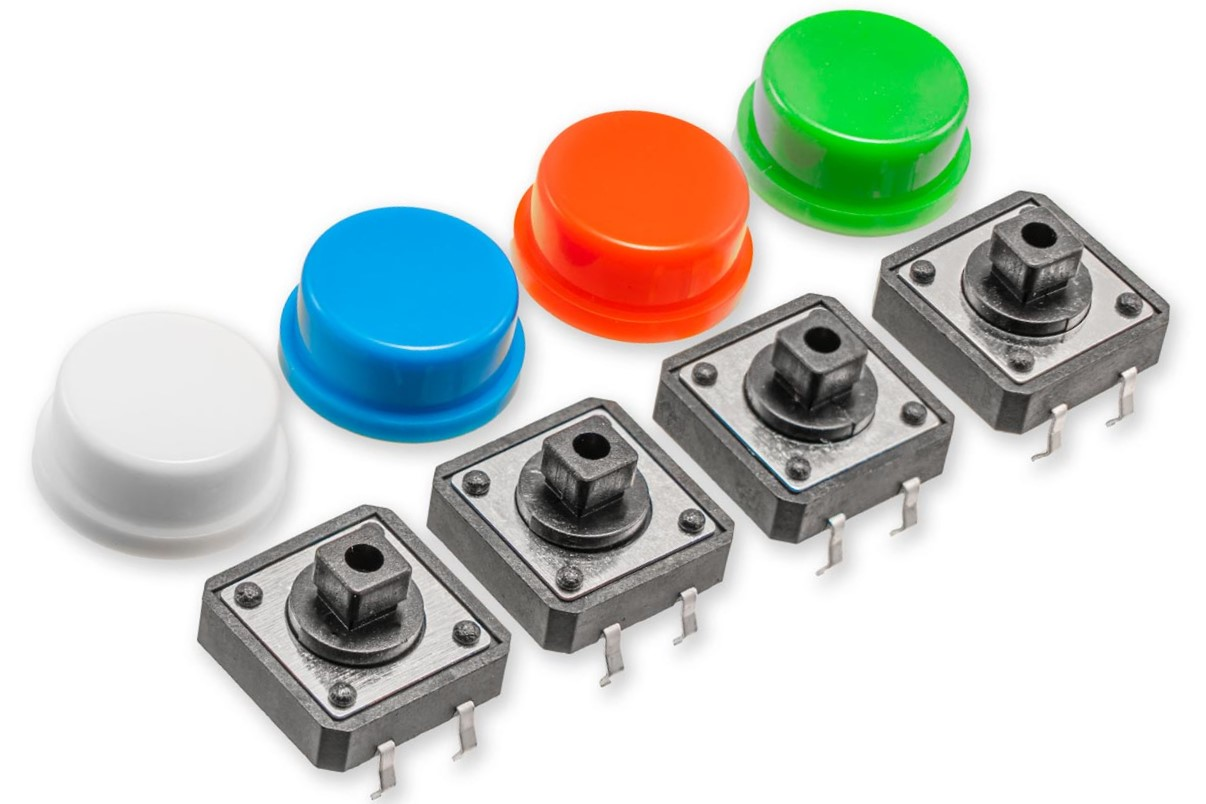
\includegraphics[width=.45\textwidth]{images/button.jpg}
    \caption{4.3mm SW button}
    \end{center} 
\end{figure}
\subsection{Variable Resistor}
The potentiometer B102 1K 16X2MM 3 Pins B162-3C102 is a type of toroidal potentiometer that is commonly used in electronic circuits for applications such as power supply, audio, and impedance matching. The "B102" in the name of the transformer indicates that it has a 1K ohm impedance, while the "16X2MM" refers to its physical size and dimensions. The three pins on the transformer are used for connecting the primary, secondary, and center-tapped windings. It uses to adjust the backlight of graphic the LCD.
\begin{figure}[H]
    \begin{center}
    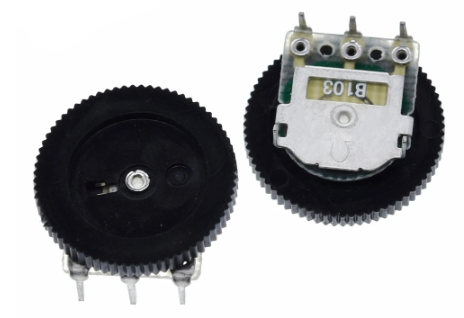
\includegraphics[width=.35\textwidth]{images/Variable_resistor.png}
    \caption{The potentiometer B102 1K 16X2MM 3 Pins B162-3C10}
    \end{center} 
\end{figure}
\section{PCB Design}
\subsection{Keypad PCB}
In this hardware design, we have implemented an $8\times 5$ keypad with a total of 40 buttons. The keypad layout consists of eight columns and five rows, providing a wide range of input options for various applications. Each button is individually connected to the corresponding column and row, enabling precise and reliable input detection.

The keypad is designed to be compact yet user-friendly, with well-spaced buttons that ensure comfortable usage. Its versatile layout allows for the inclusion of numeric digits, alphabets, symbols, and additional special function keys, catering to different requirements and user preferences.

The hardware design takes into consideration factors such as durability, responsiveness, and ease of integration. The buttons are designed to offer tactile feedback, providing users with a satisfying typing experience.

Our team designed a keypad PCB only to test with STM32F407 Discovery kit using jumper wires first for testing the code and display on the LCD to make sure that our code can run normally before uploading code to the STM32F302CCT6.

 \begin{figure}[H]
    \centering
    \subfloat[][Schematic of keypad]{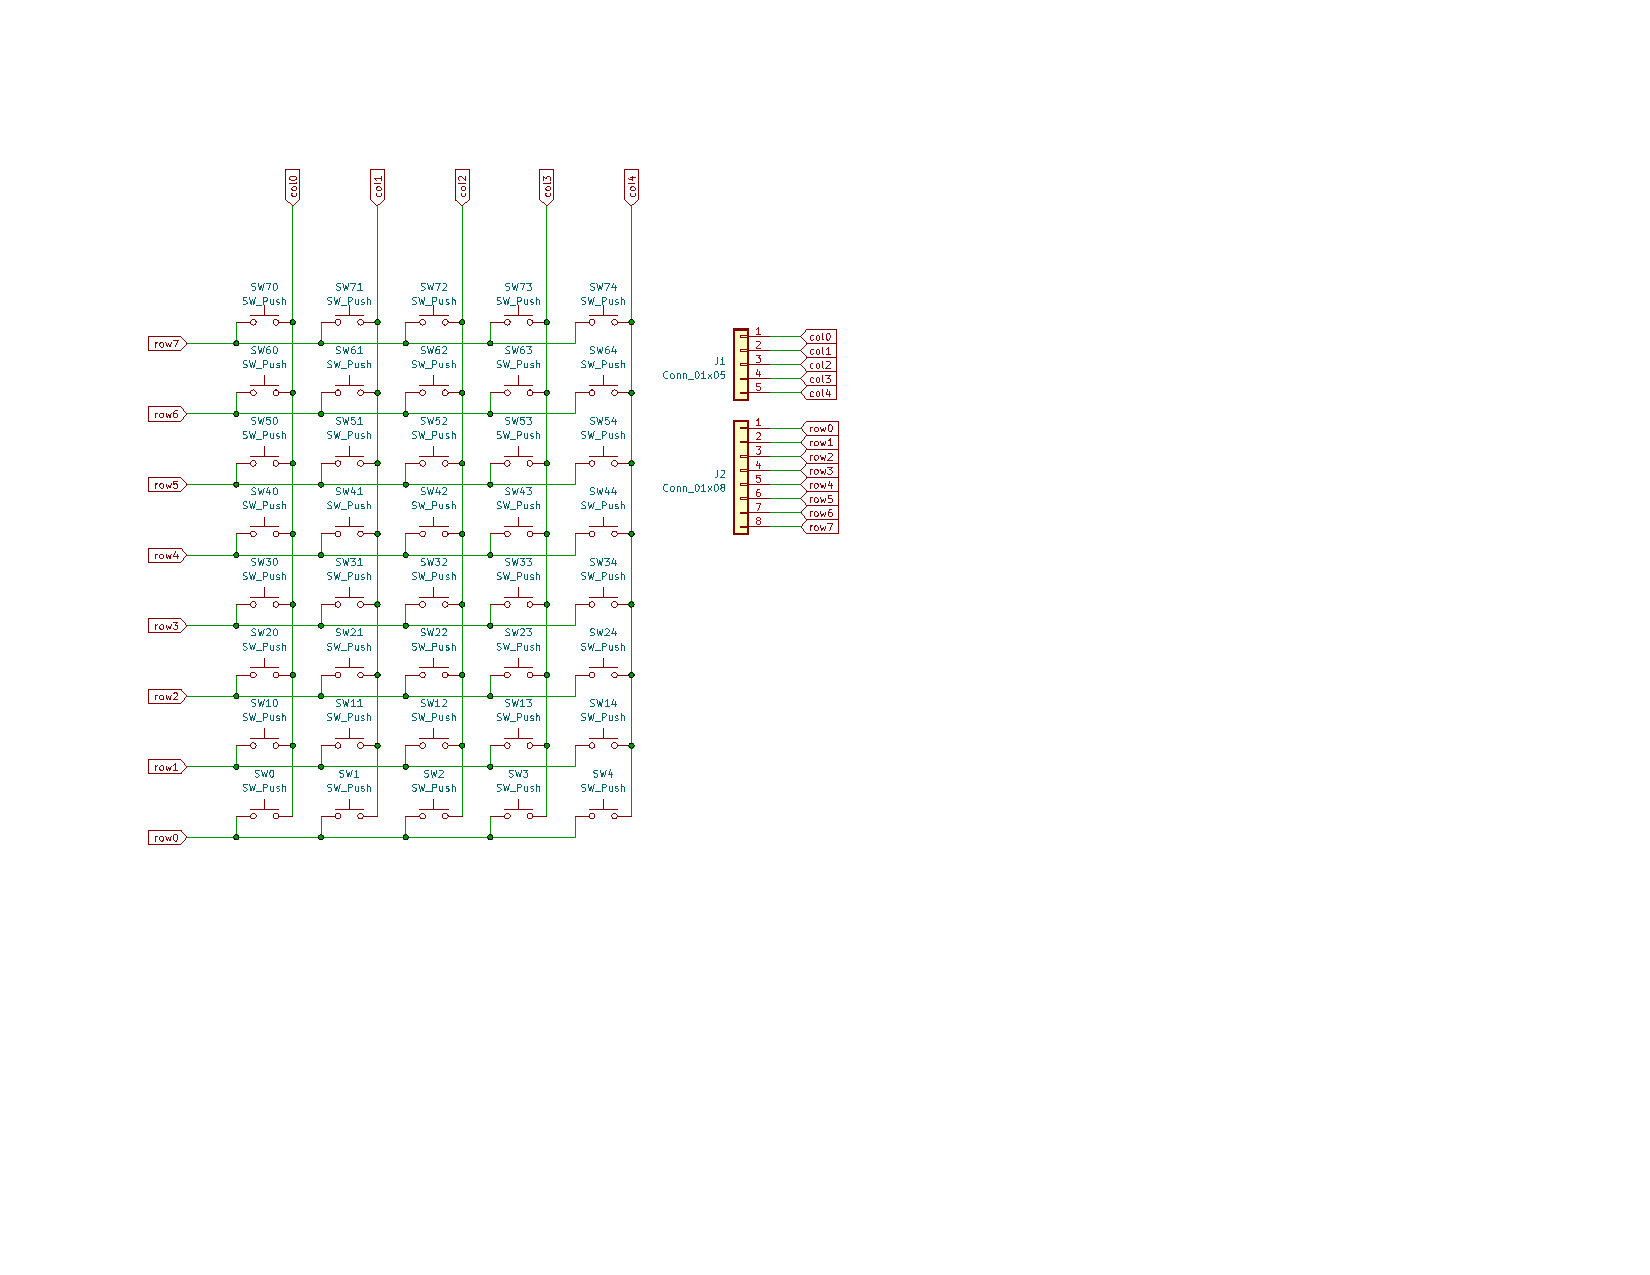
\includegraphics[width=7.5cm]{PCB/keypad_test.pdf}}\qquad
    \subfloat[][PCB of keypad]{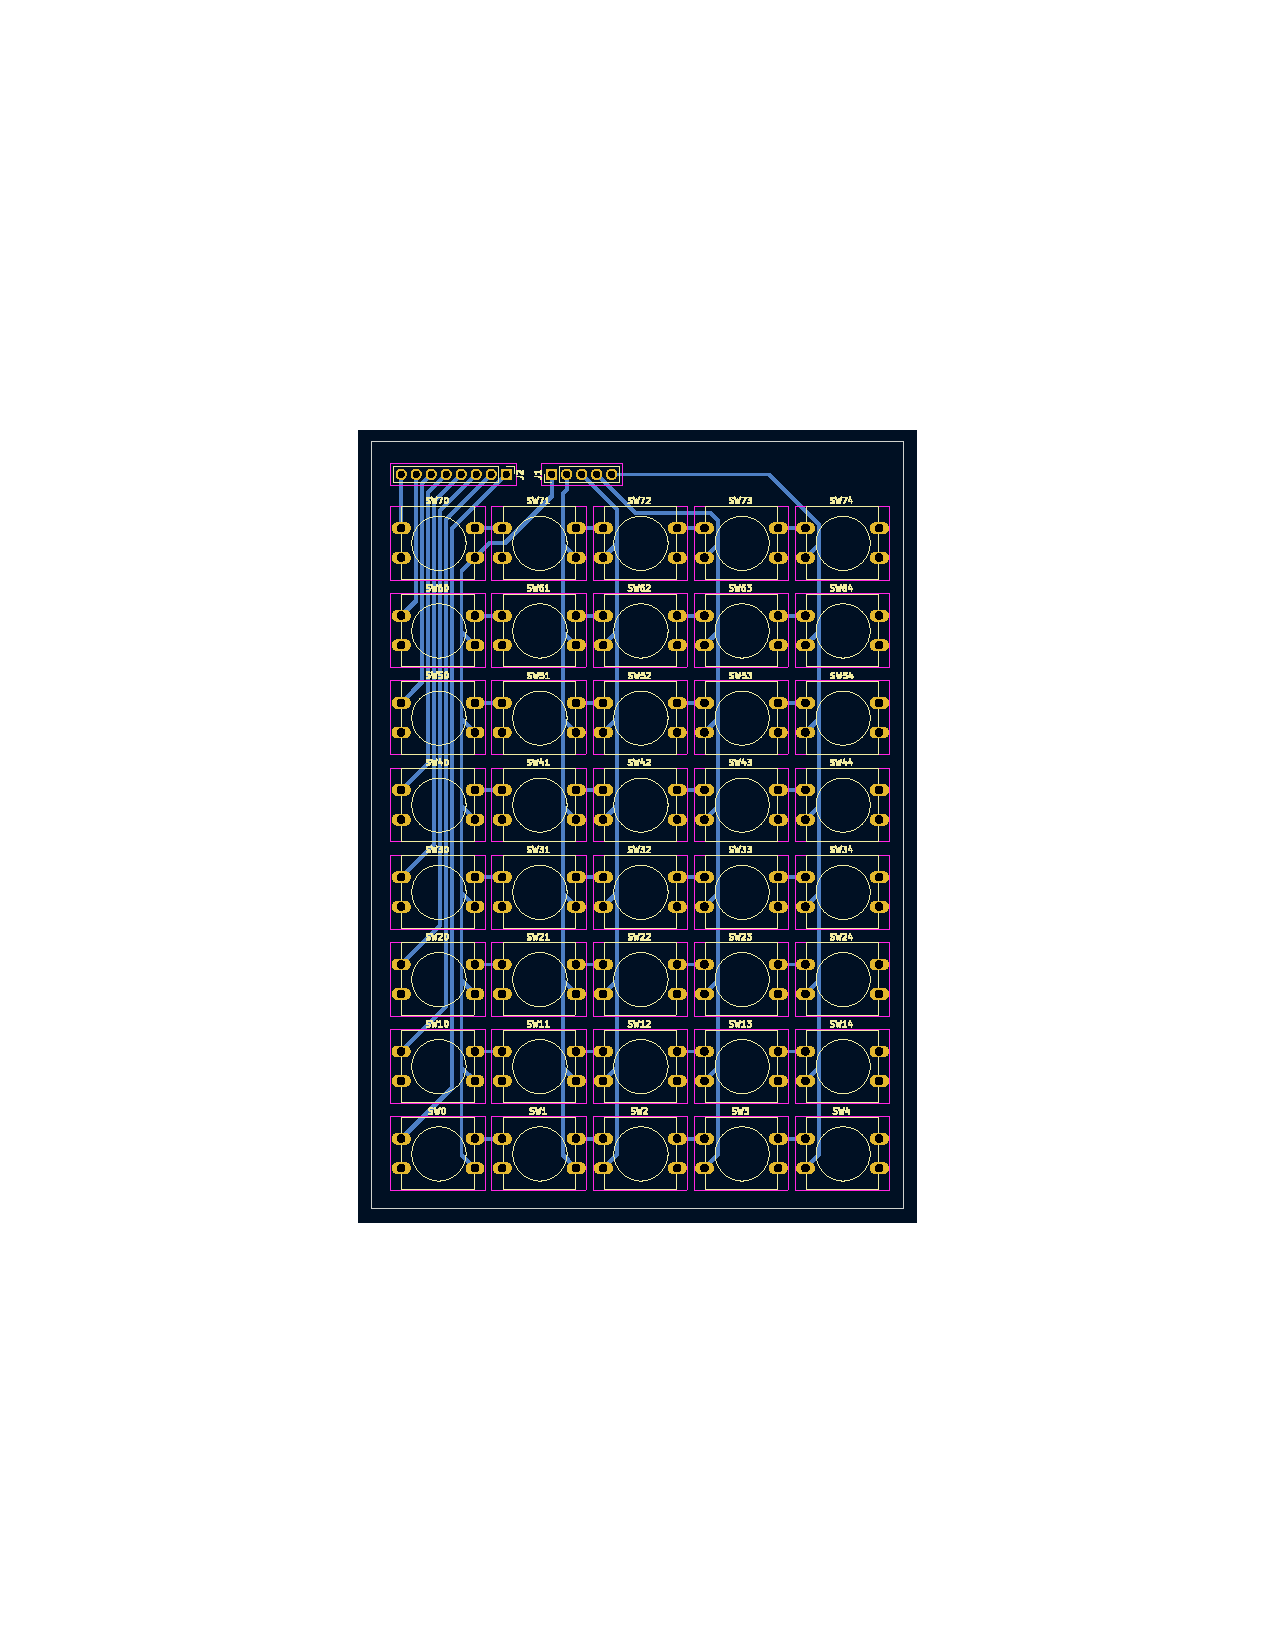
\includegraphics[width=7.5cm]{PCB/keypad_test_pcb.pdf}}
    \caption{Design of the keypad}
\end{figure}

 \begin{figure}[H]
    \centering
    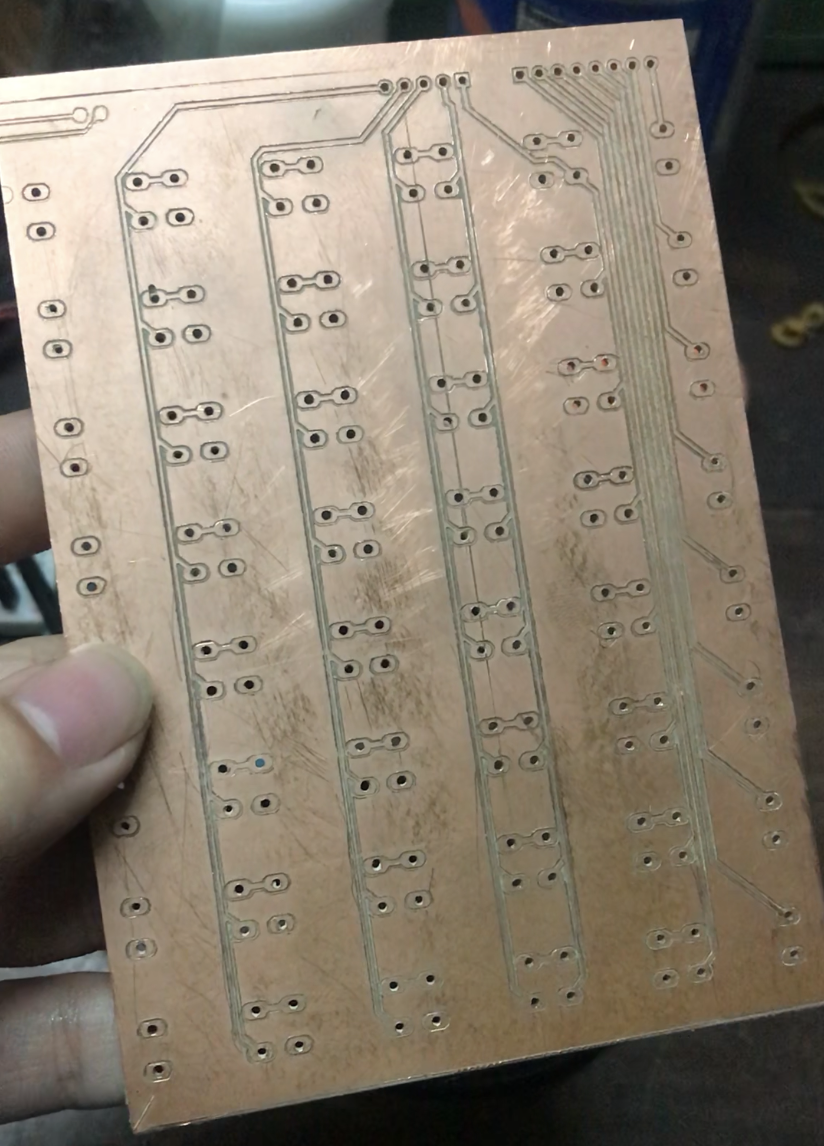
\includegraphics[width=9cm]{PCB/pcb_keypad.png}
    \caption{Keypad PCB by CNC milling}
\end{figure}

\subsection{Final design}
After conducting testing on the individual components and verifying that they were working correctly, the team proceeded to sketch the PCB layout for the entire device. This involved integrating all of the individual components, including the keypad, MCU, etc. into a single circuit board. We begin by creating a schematic diagram of the entire system, which provided a detailed overview of the various components and how they were connected.

Then we designed the PCB layout, carefully placing each component on the board and routing the necessary connections between them. We paid close attention to manufacturer's design rule such as component spacing, trace length, and signal integrity.

Due to oversight and mistakes, we unfortunately neglected to connect VDDA to 3v3 and VSSA to ground in our design. This oversight has rendered the analog-based features, including the PLL, unusable. As a result, we are left with two options for clocking: utilizing the 8MHz internal clock or incorporating a 32MHz external crystal, without the availability of PLL for additional clocking options. Recognizing this issue, we plan to modify the PCB in the future to rectify this mistake and ensure the proper connections are made. Additionally, we intend to export the NRST pin to the header to facilitate easy connection with the SWD interface.

\begin{figure}[H]
    \begin{center}
    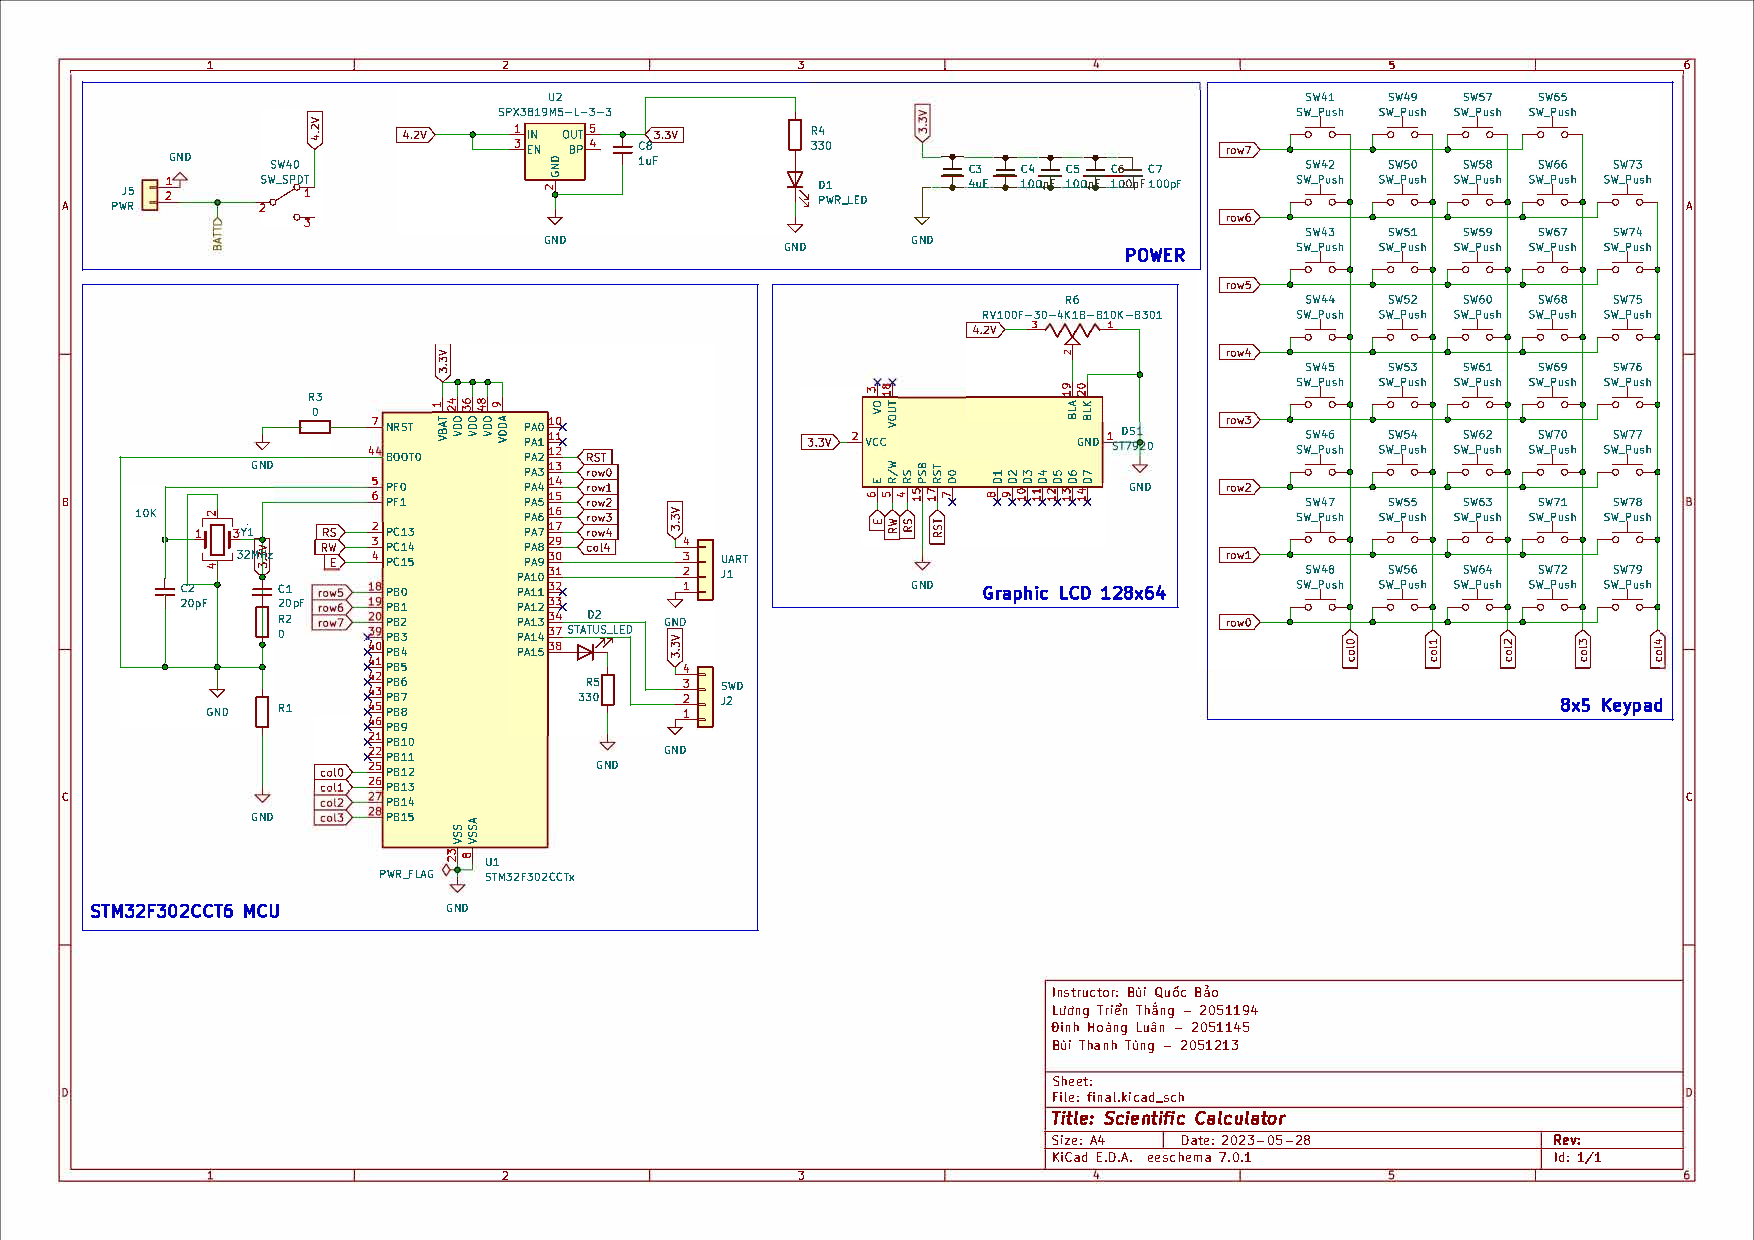
\includegraphics[trim=0.1cm 0.1cm 0.1cm 0.1cm,clip, width=.8\textwidth]{PCB/pcb_schematic.pdf}
    \caption{Schematic of the device}
    \end{center} 
\end{figure}

\begin{figure}[H]
    \begin{center}
    \subfloat[][PCB design]{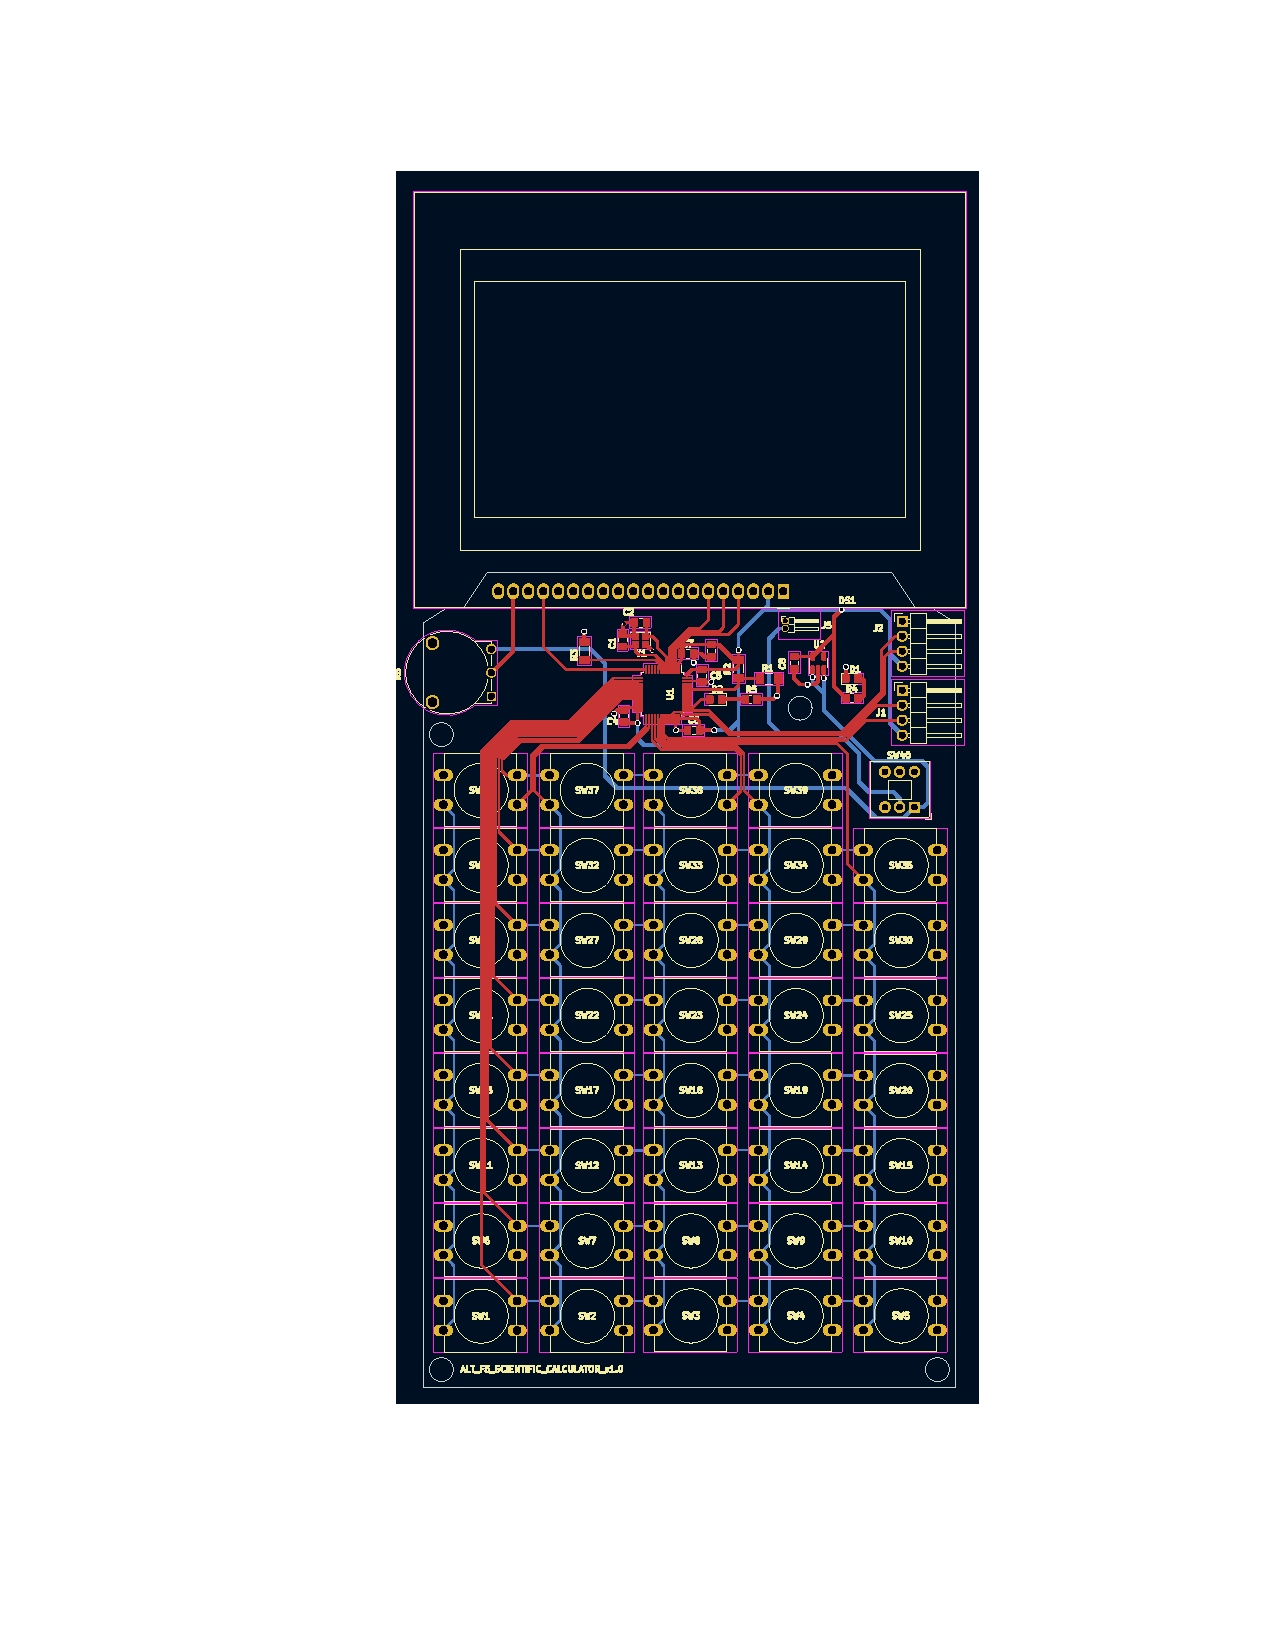
\includegraphics[width=5cm]{PCB/pcb.pdf}}\qquad
    \subfloat[][Manufactured PCB]{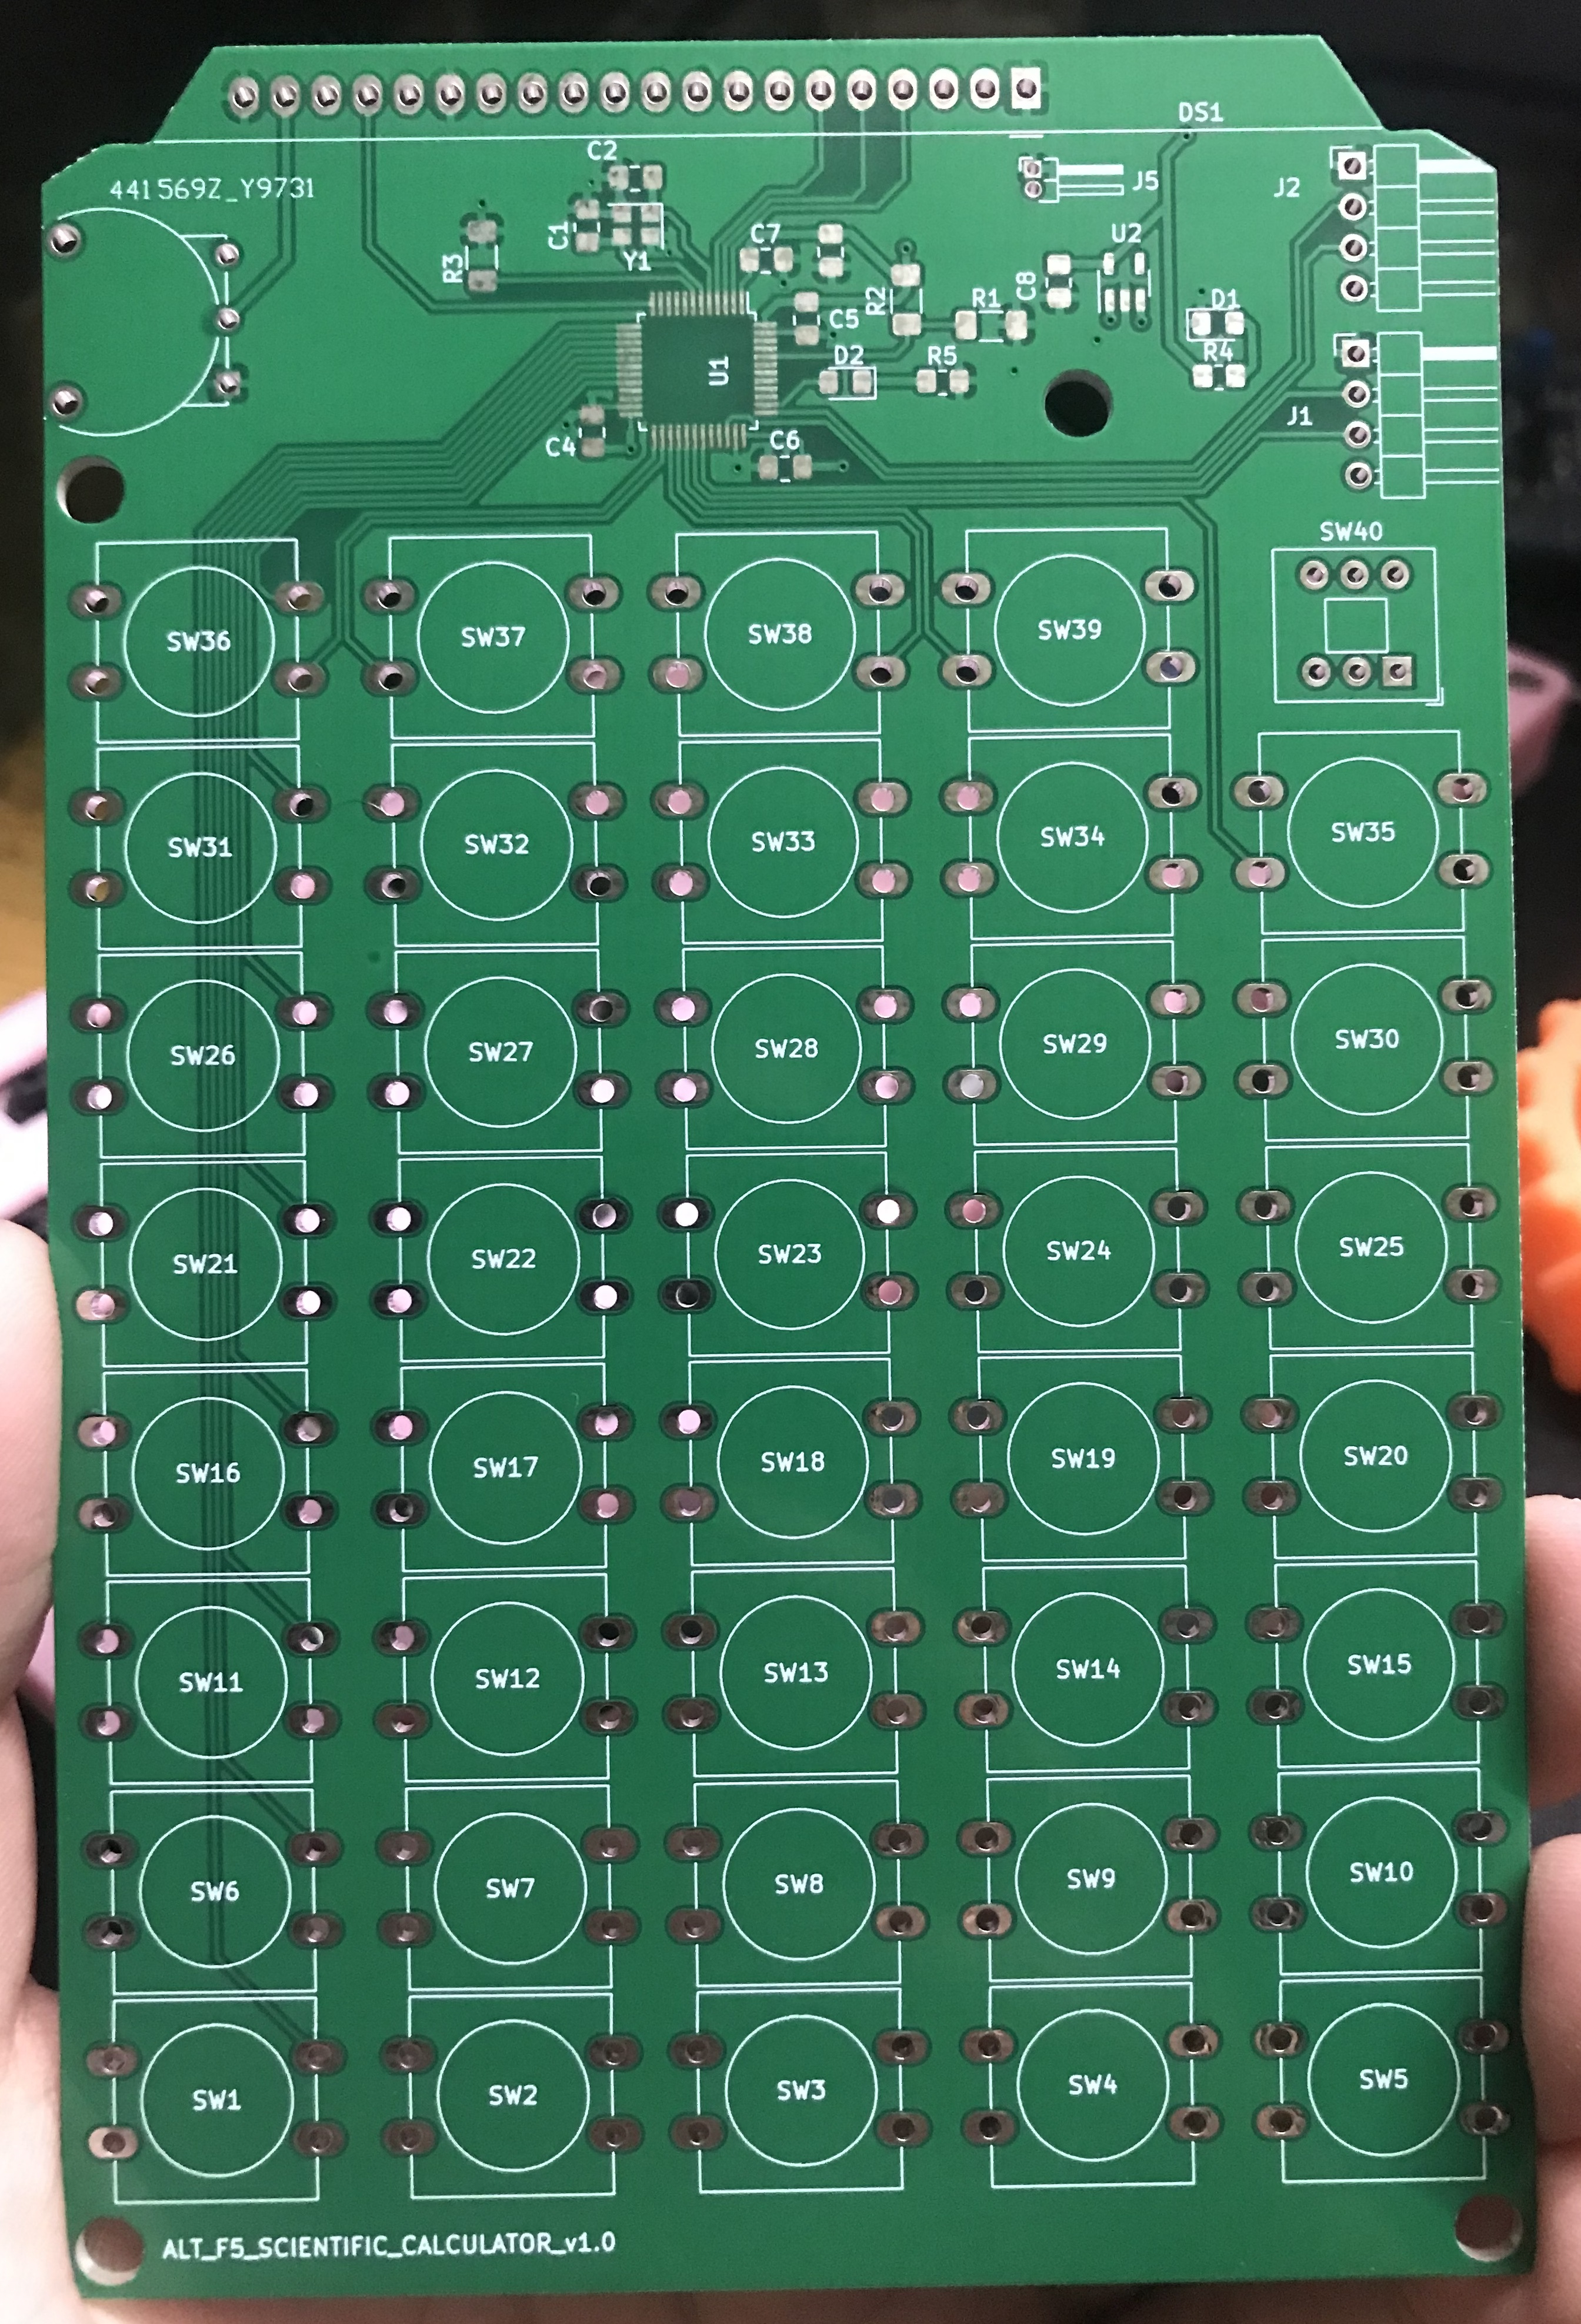
\includegraphics[width=5cm]{PCB/pcb_real.jpeg}}
    \caption{PCB Design of the device}
    \end{center} 
\end{figure}

 \begin{figure}[H]
    \centering
    \subfloat[][Front view of the PCB]{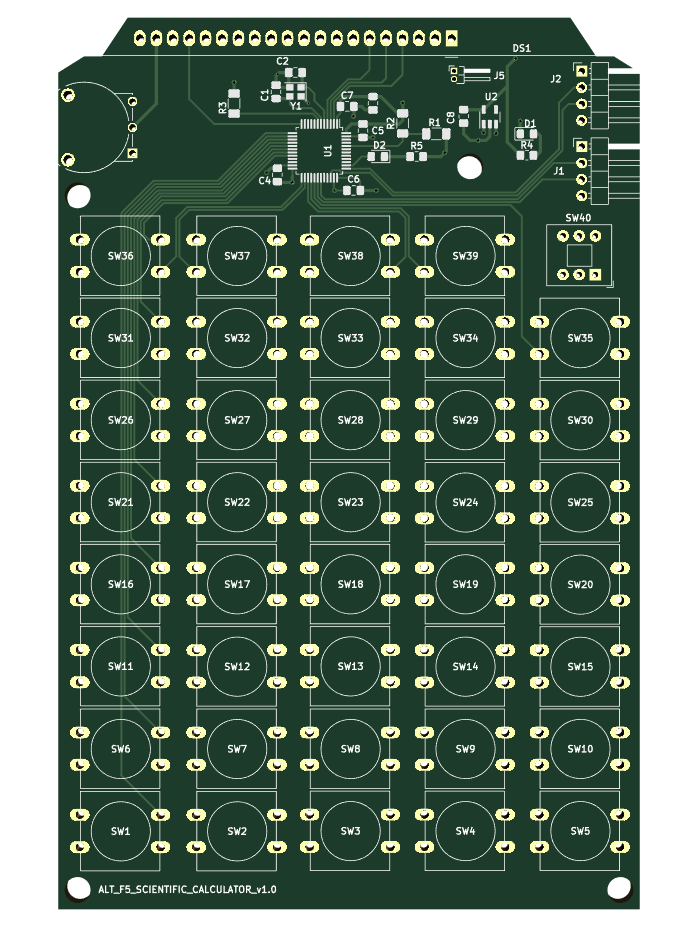
\includegraphics[width=6.5cm]{PCB/pcb_3d_front.png}}\qquad
    \subfloat[][Back view of the PCB]{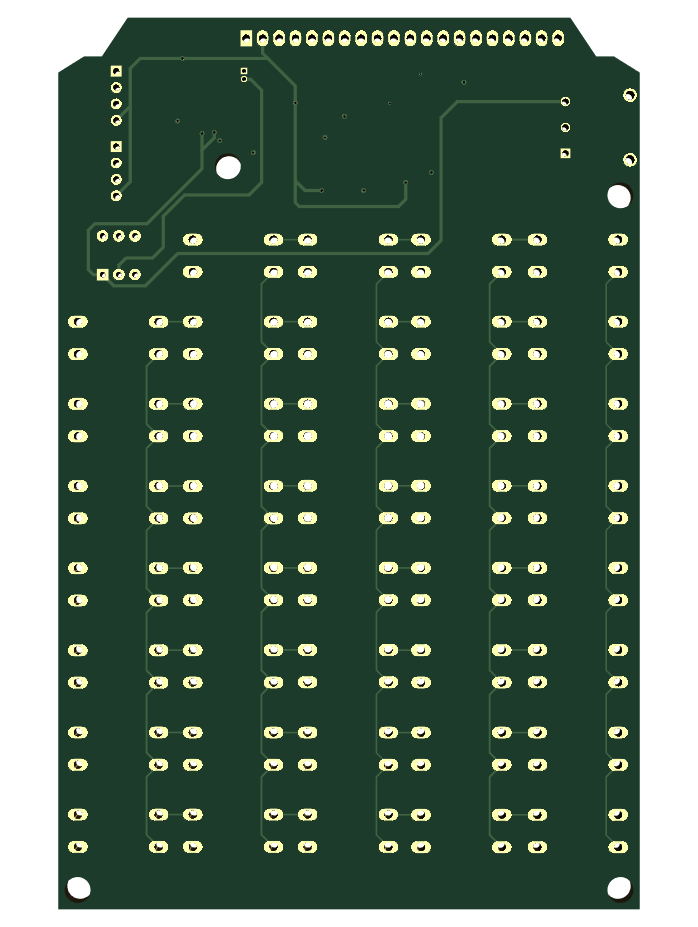
\includegraphics[width=6.5cm]{PCB/pcb_3d_back.png}}
    \caption{3D View of the PCB}
\end{figure}

The PCB of the device features two headers exposed, each serving distinct purposes. The first header is dedicated to Serial Wire Debugging (SWD), facilitating the programming and debugging of the STM32 microcontroller. SWD provides a streamlined approach to program and debug the microcontroller, ensuring efficient development and testing. The second header is designed for UART (Universal Asynchronous Receiver-Transmitter) communication, enabling seamless interaction with other devices or components such as a PC or a Wi-Fi/Bluetooth module. This UART connection allows for reliable data exchange and communication, expanding the device's capabilities for integration and connectivity.

\section{3D Printed Case}
We utilized Autodesk Fusion 360 to design a custom 3D-printed case. The case serves the purpose of enclosing and protecting various components, including the PCB, LCD screen, buttons, battery, and charging circuit. To ensure a secure fit, we divided the case into two parts: a top and a bottom. These parts are securely fastened together using screws, providing stability and protection for the internal components. Additionally, we incorporated strategically placed holes in the case to allow easy access for connecting the SWD and UART interfaces, enabling seamless programming and communication capabilities without compromising the overall functionality and aesthetics of the device.

\newpage
\begin{figure}[H]
    \centering
    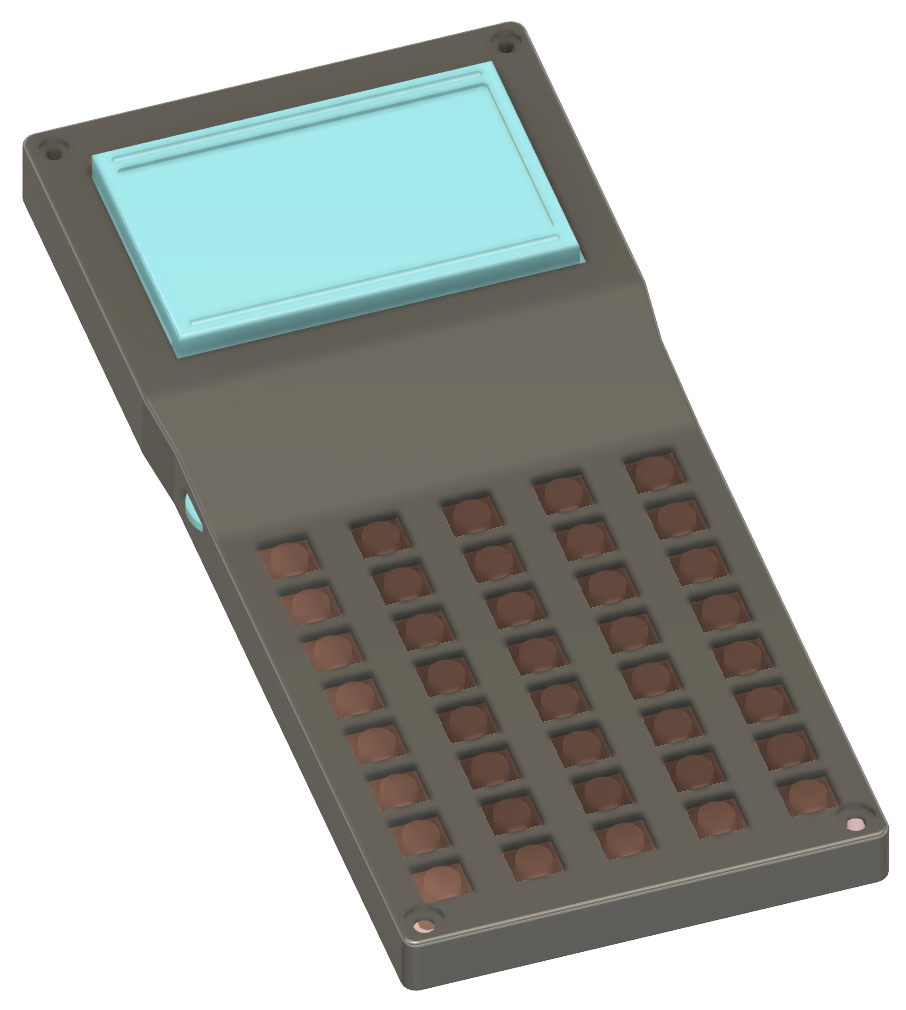
\includegraphics[width=.35\textwidth]{3DCase/all.png}
\end{figure}

\begin{figure}[H]
    \centering
    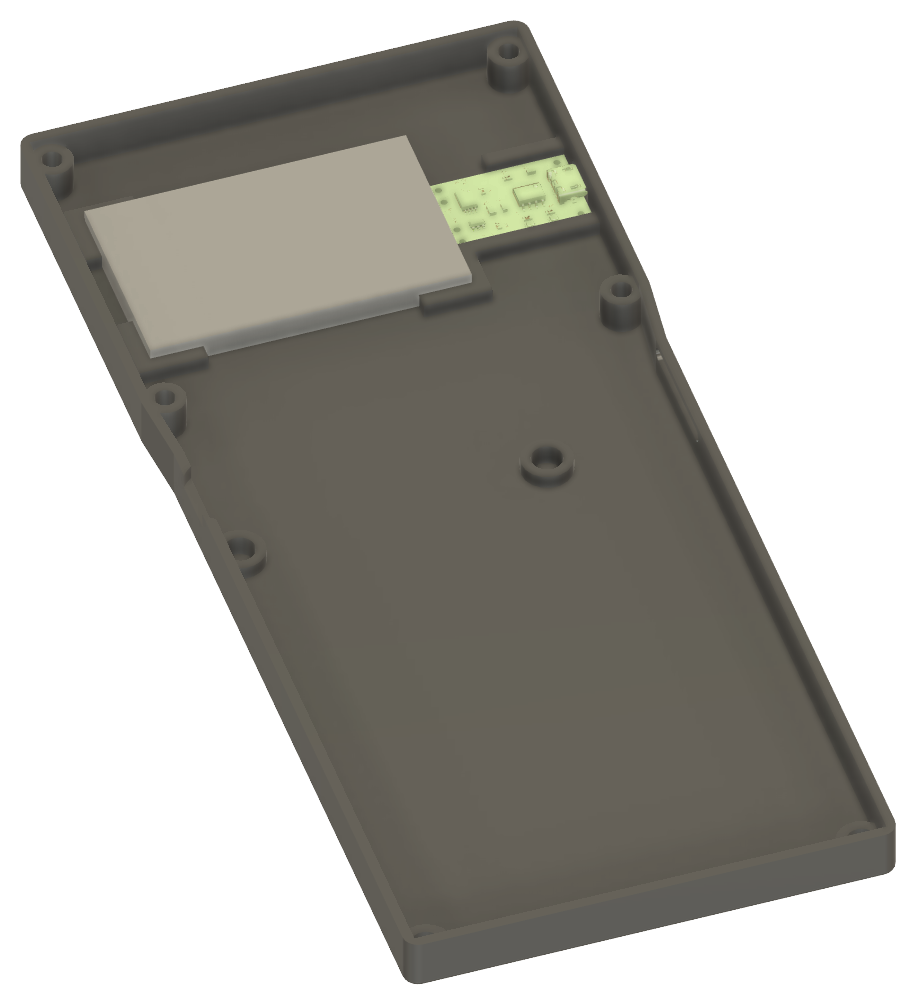
\includegraphics[width=.35\textwidth]{3DCase/bottom_with_batt.png}
    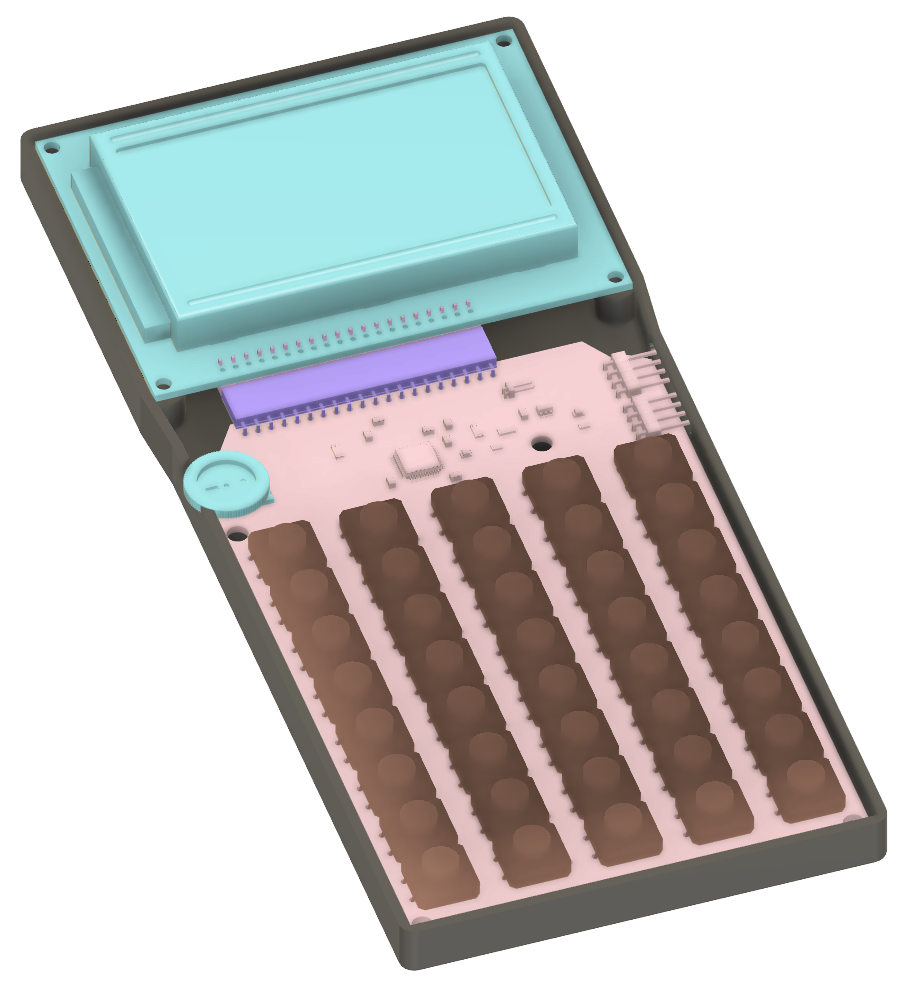
\includegraphics[width=.35\textwidth]{3DCase/bottom_and_pcb.png}
    \caption{The device with case}
\end{figure}

\begin{figure}[H]
    \centering
    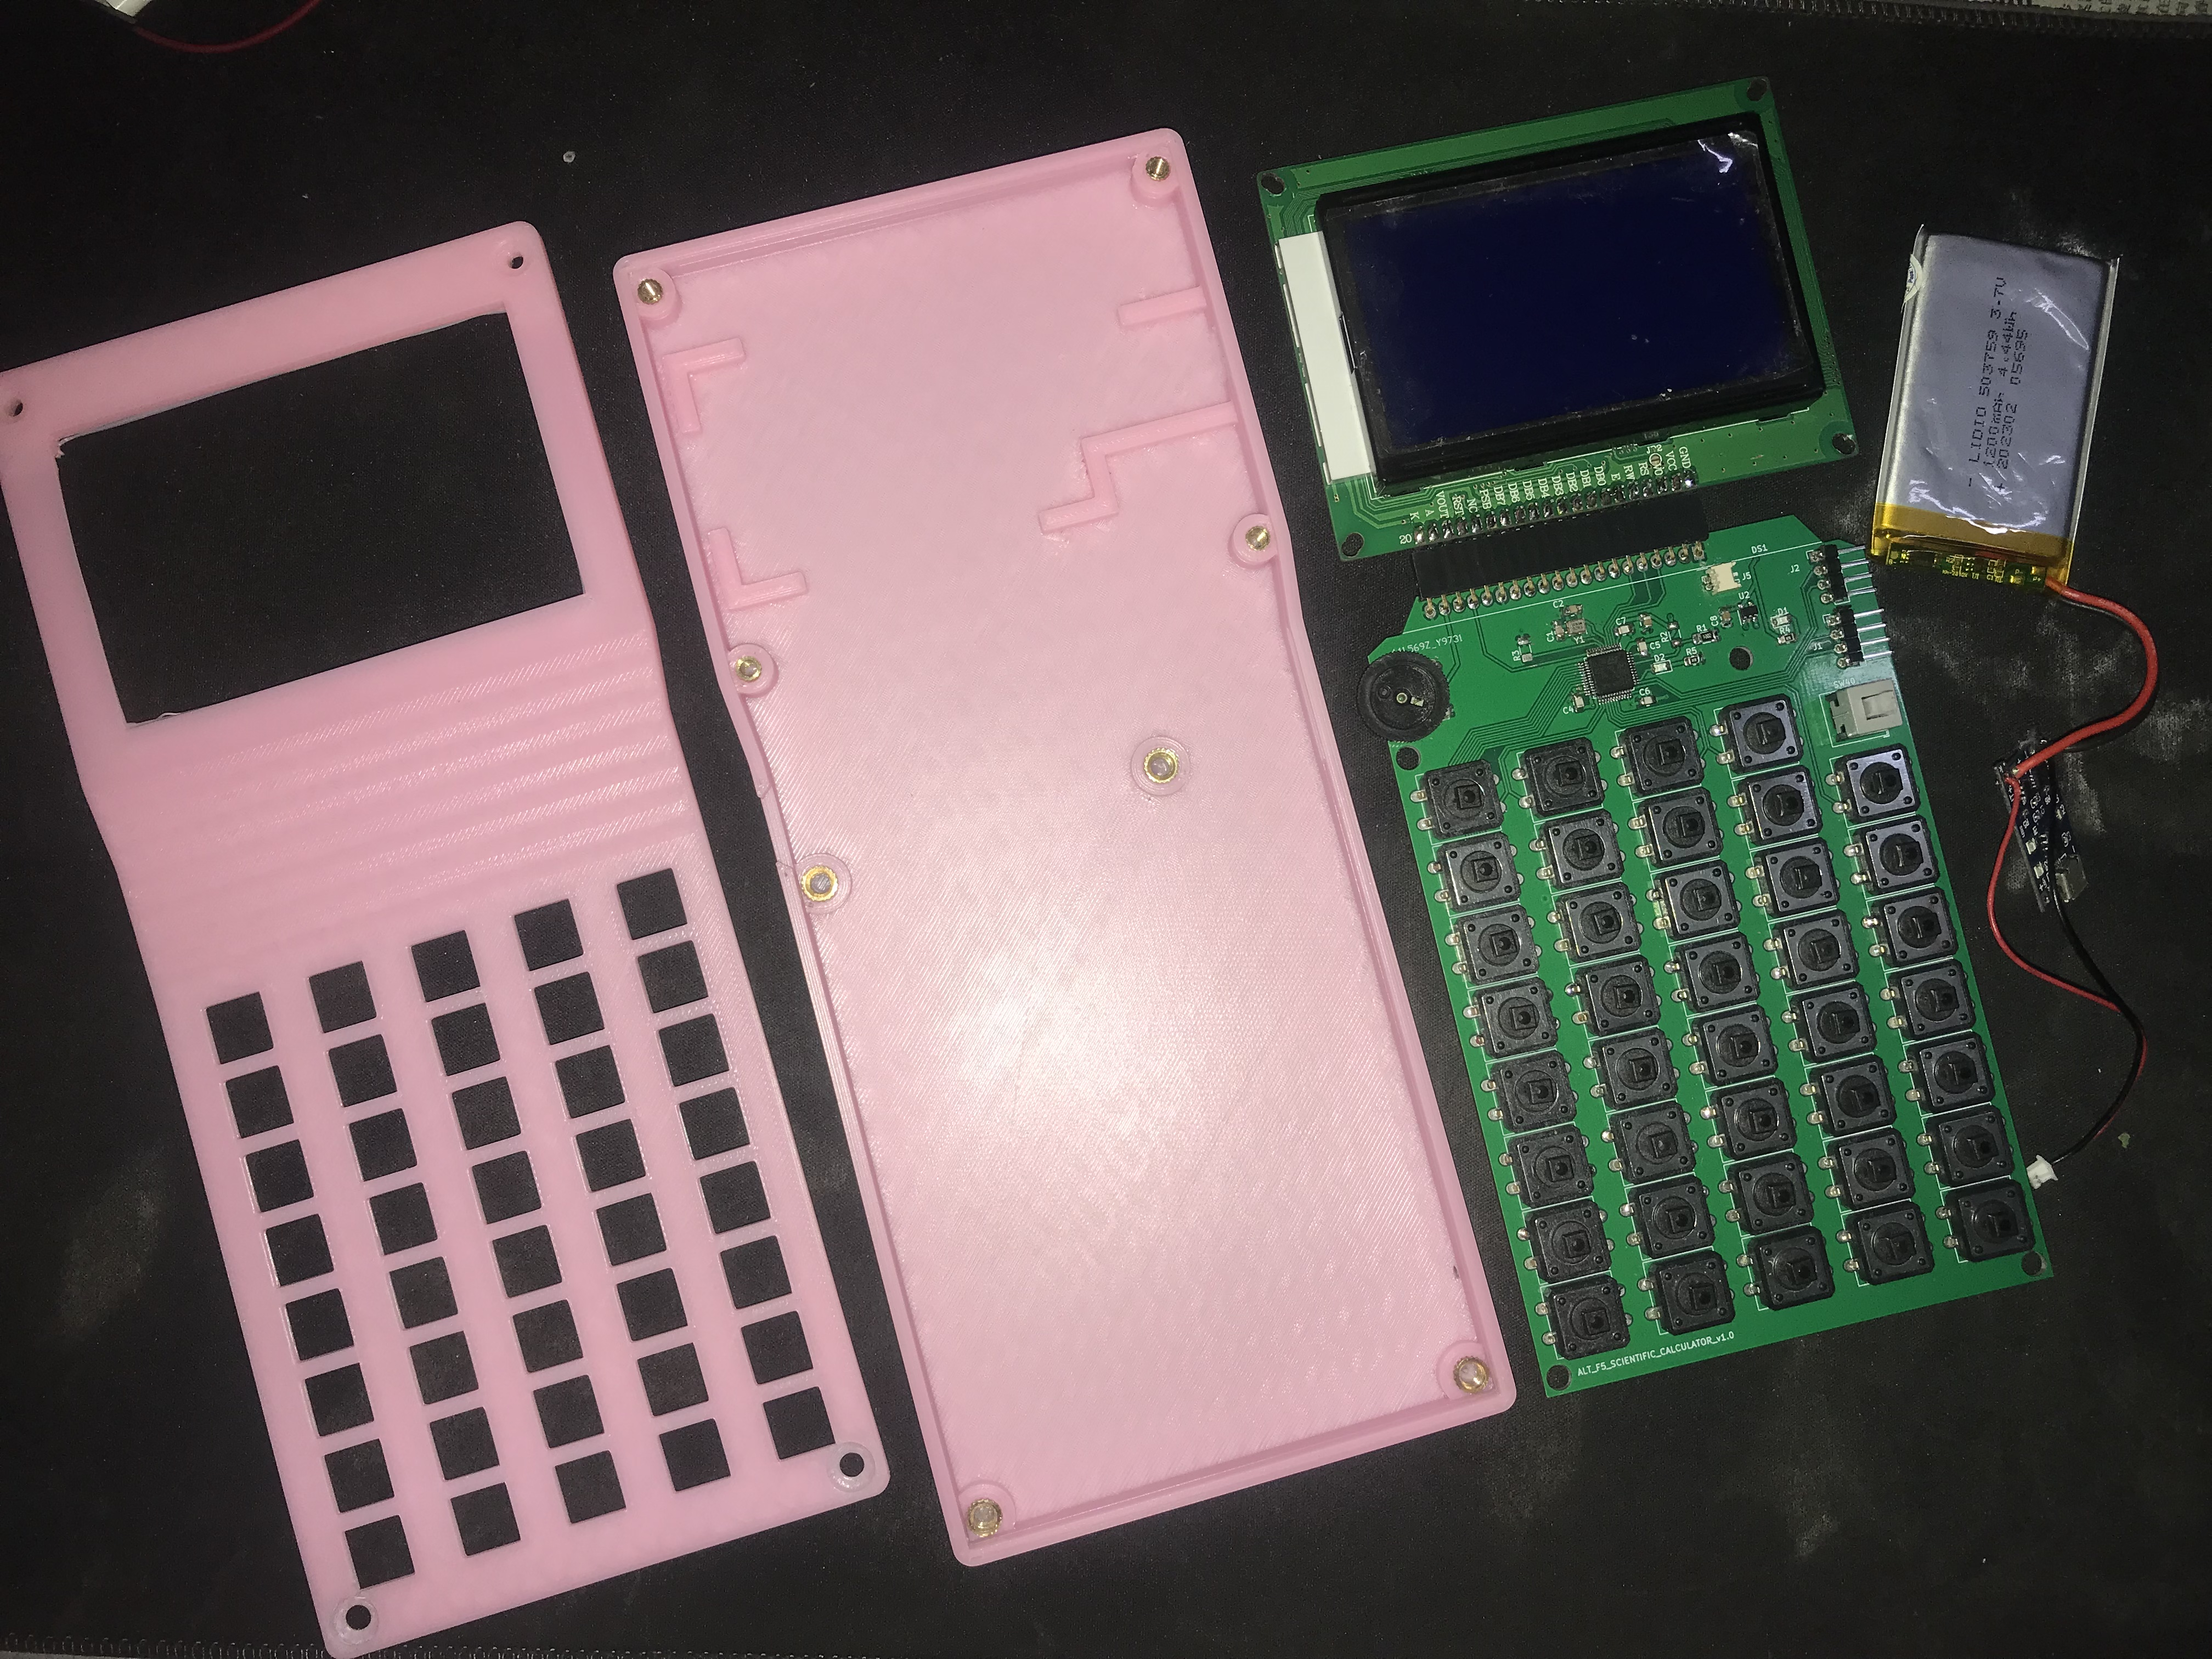
\includegraphics[width=.6\textwidth]{3DCase/3dprinted.jpeg}
    \caption{3D Printed Case}
\end{figure}

\chapter{Software}
\section{HAL Library}
The HAL (Hardware Abstraction Layer) library for STM32 microcontrollers is a set of functions provided by STMicroelectronics, the manufacturer of STM32 microcontrollers, to simplify the development of applications for these devices. The HAL library abstracts the low-level details of the microcontroller's hardware, allowing developers to write portable code that can be used across different STM32 microcontroller models.

The HAL library provides a wide range of functions that cover various aspects of microcontroller programming, including GPIO (General Purpose Input/Output), timers, UART (Universal Asynchronous Receiver/Transmitter), SPI (Serial Peripheral Interface), I2C (Inter-Integrated Circuit), DMA (Direct Memory Access), and more. These functions provide a higher level of abstraction compared to directly manipulating the microcontroller's registers, making it easier to configure and use the hardware peripherals.

In contrast, register-based programming involves directly manipulating microcontroller registers for fine-grained control and optimization, requiring a deeper understanding of hardware details but offering more customization. The choice depends on familiarity with hardware, project complexity, portability needs, and desired level of control and optimization.

In summary, choosing the HAL (Hardware Abstraction Layer) approach over register-based programming for STM32 microcontrollers is generally recommended. HAL provides an intuitive API, portability, and ease of use, while register-based programming offers more control and customization at the cost of complexity and reduced portability. But register-based programming is also used to increase the performance of the microcontroller.

\section{Interaction with hardware}
\subsection{Keypad Scanning}
The keypad scanning method is a technique used to detect and interpret input from a keypad or keyboard. It is commonly employed in various electronic devices such as calculators, mobile phones, and security systems. This method allows the device to determine which keys are pressed and subsequently process the corresponding input.

\begin{figure}[H] % http://esd.cs.ucr.edu/labs/decode_key/decode_key.html
    \centering
    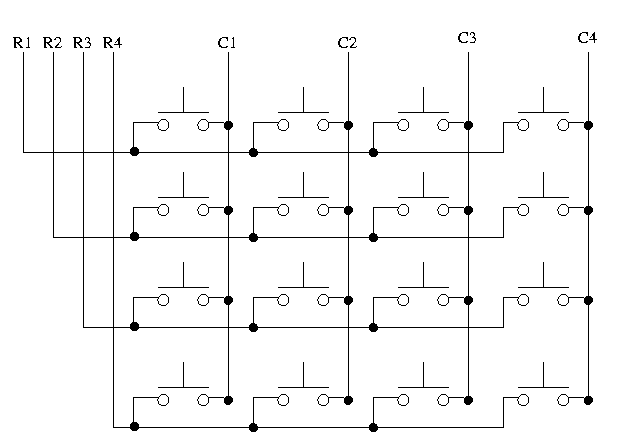
\includegraphics[width=.9\textwidth]{images/keypad.png}
    \caption{$4\times 4$ Keypad Schematic}
\end{figure}

In a typical keypad scanning system, the rows and columns of buttons are connected to a microcontroller or dedicated scanning circuitry. Here's a step-by-step breakdown of the process:

\begin{enumerate}
    \item Initializing Process: The scanning process begins by initializing the rows and columns as inputs to the microcontroller or scanning circuitry.
    \item Row Scanning: The scanning starts with all rows in an inactive state. The microcontroller sequentially activates one row at a time by setting it to a logic high (or low) state. The other rows remain in an inactive state.
    \item Column Detection: With a row activated, the microcontroller scans the state of each column. It checks if any buttons in the active row are pressed. This is done by checking the logic level of the corresponding column pins.
    \begin{itemize}
        \item If a button in the active row is pressed, it establishes an electrical connection between the active row and the corresponding column. The microcontroller detects this change in continuity.
        \item If a button in the active row is not pressed, there is no continuity between the active row and the corresponding column.
    \end{itemize}
    \item Button Identification: If the microcontroller detects a pressed button, it records the intersection point between the active row and the detected column. This intersection represents the specific button that was pressed.
    \item Data Processing: Once the button is identified, the microcontroller processes the recorded button press information. It may use lookup tables or algorithms to determine the corresponding character or function associated with the pressed button. The device then performs the appropriate action or displays the input on the screen.
    \item Repeating the Process: After processing the current button press, the scanning process continues by deactivating the current row and moving to the next row. The same detection and processing steps are repeated for each row and its corresponding columns until all buttons have been scanned.
\end{enumerate}

Here is the code that demonstrates the keypad scanning for STM32. The function supports checking if the users holding the button. The function will return \texttt{0xFFFF} if no key is pressed, and return the corresponding coordinates \texttt{0xrrcc} (row, column) if a key is pressed.

\begin{minted}{C}
uint16_t KeyPad_Scan(bool GetKeyHold) {
  uint16_t key = 0;
  for (uint8_t c = 0; c < KeyPad.ColumnSize; c++) {
    for (uint8_t i = 0; i < KeyPad.ColumnSize; i++) {
    	((GPIO_TypeDef*)(_KEYPAD_COLUMN_GPIO_PORT[i]))->BSRR = (uint32_t)_KEYPAD_COLUMN_GPIO_PIN[i];
    }

	((GPIO_TypeDef*)(_KEYPAD_COLUMN_GPIO_PORT[c]))->BRR = (uint32_t)_KEYPAD_COLUMN_GPIO_PIN[c];
    _KEYPAD_DELAY(5);
    for (uint8_t r = 0; r < KeyPad.RowSize; r++) {
      if ((((GPIO_TypeDef * )_KEYPAD_ROW_GPIO_PORT[r])->IDR & (uint32_t)_KEYPAD_ROW_GPIO_PIN[r]) == GPIO_PIN_RESET) {
        _KEYPAD_DELAY(_KEYPAD_DEBOUNCE_TIME_US);
        if ((((GPIO_TypeDef * )_KEYPAD_ROW_GPIO_PORT[r])->IDR & (uint32_t)_KEYPAD_ROW_GPIO_PIN[r]) == GPIO_PIN_RESET) {
          key |= r;
          key = (key << 8) | c;
          if (!GetKeyHold)
            while((((GPIO_TypeDef * )_KEYPAD_ROW_GPIO_PORT[r])->IDR & (uint32_t)_KEYPAD_ROW_GPIO_PIN[r]) == GPIO_PIN_RESET)
              _KEYPAD_DELAY(5);
          return key;
        }
      }
    }
  }
  return 0xFFFF;
}
\end{minted}

\newpage
\begin{table}[H]
    \centering
    \begin{tabular}{|l|l|l|l|l|l|l|}
    \hline
        \textbf{Key} & \textbf{Function} & \textbf{Alt. Function} & \textbf{} & \textbf{Key} & \textbf{Function} & \textbf{Alt. Function} \\ \hline
        0x0000 & 0 & $+\inf$, $-\inf$ & ~ & 0x0400 & ! & ~ \\ \hline
        0x0001 & . & , & ~ & 0x0401 & ( & ~ \\ \hline
        0x0002 & $\hat{}$ & $\sqrt{\text{ }}$, $\sqrt[n]{\text{ }}$ & ~ & 0x0402 & ) & ~ \\ \hline
        0x0003 & Ans & ~ & ~ & 0x0403 & sin & cos, tan \\ \hline
        0x0004 & $=$ & ~ & ~ & 0x0404 & S2D & ~ \\ \hline\hline
        0x0100 & 1 & ~ & ~ & 0x0500 & ~ & ~ \\ \hline
        0x0101 & 2 & ~ & ~ & 0x0501 & abs & ~ \\ \hline
        0x0102 & 3 & ~ & ~ & 0x0502 & ~ & ~ \\ \hline
        0x0103 & + & ~ & ~ & 0x0503 & lim & d/dx, int \\ \hline
        0x0104 & - & ~ & ~ & 0x0504 & ln & log, logx \\ \hline\hline
        0x0200 & 4 & ~ & ~ & 0x0600 & == & ~ \\ \hline
        0x0201 & 5 & ~ & ~ & 0x0601 & LEFT & ~ \\ \hline
        0x0202 & 6 & ~ & ~ & 0x0602 & DOWN & ~ \\ \hline
        0x0203 & $\times$ & ~ & ~ & 0x0603 & RIGHT & ~ \\ \hline
        0x0204 & / & ~ & ~ & 0x0604 & $x$ & $y$, $z$ \\ \hline\hline
        0x0300 & 7 & ~ & ~ & 0x0700 & ~ & ~ \\ \hline
        0x0301 & 8 & ~ & ~ & 0x0701 & ~ & ~ \\ \hline
        0x0302 & 9 & ~ & ~ & 0x0702 & UP & ~ \\ \hline
        0x0303 & BS & ~ & ~ & 0x0703 & MODE & ~ \\ \hline
        0x0304 & AC & ~ & ~ & 0x0704 & PWR & ~ \\ \hline
    \end{tabular}
    \caption{Keypad keys mapping}
\end{table}

\subsection{LCD ST7920 Communication}
The ST7920 is a popular LCD controller chip used in certain types of graphical LCD displays. It is commonly used in conjunction with an 128x64 pixel graphical LCD module. The ST7920 chip supports the parallel interface mode for communication with microcontrollers or other devices.

\subsubsection{Setup Timer}
The timer module in STM32 microcontrollers provides precise timing capabilities, allowing developers to implement various time-based functionalities in their applications. One common application of the timer module is to generate interrupts at regular intervals, such as every second. 

To use timer, simply set the clock source of the timer to internal clock, setup the prescaler and counter value.

\newpage
\begin{figure}[H]
    \centering
    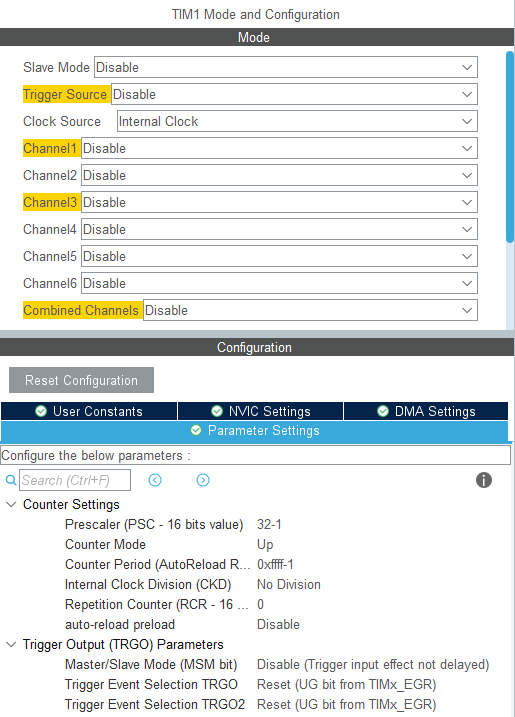
\includegraphics[width=.6\textwidth]{images/Timer_Config.png}
    \caption{Timer configuration for precise timing}
\end{figure}

The prescaler is a configurable value that divides the clock frequency to produce a lower frequency input for the timer. By dividing the clock frequency, the prescaler allows for finer control over the timer's resolution. In our case, with a 32 MHz clock and a prescaler value of 32-1, the clock frequency is divided by 32, resulting in a reduced frequency of 1 MHz.

The counter period, on the other hand, sets the maximum value the timer can count up to before it wraps around and generates an interrupt or triggers an event. By setting a counter period, you define the duration for which the timer will count before reaching its maximum value. In our case, with a counter period of 0xff-1, the timer will count from 0 to 0xff before resetting.

In summary, by setting the prescaler to 32-1 and the counter period to 0xff-1, we achieve a timer frequency of 1 MHz, and the timer will generate an interrupt or trigger an event every microsecond. This configuration allows us to precisely time events or perform periodic tasks in our application.

\subsubsection{Send data to ST7920}
The ST7920 controller chip typically supports both parallel and serial communication interfaces. In addition to the parallel interface mode, it can also operate in software SPI (Serial Peripheral Interface) mode.

It's important to note that implementing software SPI requires careful attention to timing, so we used a timer to create a precise timing delay for the communication.
\begin{minted}{C}
void delay_us(uint16_t delay) {
  __HAL_TIM_SET_COUNTER( & htim1, 0); // reset the counter
  while ((__HAL_TIM_GET_COUNTER( & htim1)) < delay) ; // wait for the delay to complete
}
\end{minted}

The sending data functions below is based on the demo program written in assembly that introduced in the datasheet. \footfullcite[][27]{st7920_datasheet}
\begin{minted}{C}
void SendByteSPI(uint8_t byte) {
  for (int i = 0; i < 8; i++) {
    if ((byte << i) & 0x80) {
    	SID_PORT->BSRR = SID_PIN;           // SID=1  OR MOSI
    } else {
    	SID_PORT->BRR = SID_PIN;        // SID=0
    }
    SCLK_PORT->BRR = SCLK_PIN;                  // SCLK =0  OR SCK
    SCLK_PORT->BSRR = SCLK_PIN;                 // SCLK=1
  }
}

void ST7920_SendCmd(uint8_t cmd) {
  CS_PORT -> BSRR = CS_PIN;                     // Pull the CS high

  SendByteSPI(0xf8 + (0 << 1));                 // send the SYNC + RS(0)
  SendByteSPI(cmd & 0xf0);                      // send the higher nibble first
  SendByteSPI((cmd << 4) & 0xf0);               // send the lower nibble
  delay_us(50);

  CS_PORT -> BRR = CS_PIN;                      // Pull the CS LOW

}

void ST7920_SendData(uint8_t data) {
  CS_PORT -> BSRR = CS_PIN;                     // Pull the CS high

  SendByteSPI(0xf8 + (1 << 1));                 // send the SYNC + RS(1)
  SendByteSPI(data & 0xf0);                     // send the higher nibble first
  SendByteSPI((data << 4) & 0xf0);              // send the lower nibble
  delay_us(50);

  CS_PORT -> BRR = CS_PIN;                      // Pull the CS LOW
}
\end{minted}

\subsubsection{Initialize the LCD}
Initializing an LCD module with an ST7920 controller is important to configure the display parameters, establish communication, set memory and state, and ensure compatibility and stability. It prepares the display for displaying text or graphics by setting up the necessary settings, clearing memory, and synchronizing the microcontroller with the controller. Proper initialization ensures reliable operation and accurate content display on the LCD module. Here is a function for initializing the LCD based on the datasheet. \footfullcite[][34]{st7920_datasheet}

\begin{minted}{C}
void ST7920_Init(void) {
  delay_init();
  RST_PORT -> BRR = RST_PIN;            // RESET=0
  HAL_Delay(10); // wait for 10ms
  RST_PORT -> BSRR = RST_PIN;           // RESET=1

  HAL_Delay(50);                        //wait for >40 ms

  ST7920_SendCmd(0x30);                 // 8bit mode
  delay_us(110);                        //  >100us delay

  ST7920_SendCmd(0x30);                 // 8bit mode
  delay_us(40);                         // >37us delay

  ST7920_SendCmd(0x08);                 // D=0, C=0, B=0
  delay_us(110);                        // >100us delay

  ST7920_SendCmd(0x01);                 // clear screen
  HAL_Delay(12);                        // >10 ms delay

  ST7920_SendCmd(0x06);                 // cursor increment right no shift
  HAL_Delay(1);                         // 1ms delay

  ST7920_SendCmd(0x0C);                 // D=1, C=0, B=0
  HAL_Delay(1);                         // 1ms delay

  ST7920_SendCmd(0x02);                 // return to home
  HAL_Delay(1);                         // 1ms delay
}
\end{minted}

\subsubsection{Enable/Disable Graphics mode}
The ST7920 controller supports a graphics mode that allows you to render graphical content on an LCD display connected to the controller. In graphics mode, you can draw lines, circles, rectangles, and other shapes on the display, which means we can handle every single pixel in the LCD buffer. \footfullcite[][17]{st7920_datasheet}

\begin{minted}{C}
void ST7920_GraphicMode(int enable) {   // 1-enable, 0-disable
  if (enable == 1) {
    ST7920_SendCmd(0x30);               // 8 bit mode
    delay_us(80);
    ST7920_SendCmd(0x34);               // switch to Extended instructions
    delay_us(80);
    ST7920_SendCmd(0x36);               // enable graphics
    delay_us(80);
  } else if (enable == 0) {
    ST7920_SendCmd(0x30);               // 8 bit mode
    delay_us(80);
  }
}
\end{minted}

\subsubsection{Graphic Display RAM}
The ST7920 LCD display has a resolution of 128 pixels (width) by 64 pixels (height). The display is divided into two halves vertically, with the upper half having a Y-coordinate range of 0 to 31 and the lower half having a Y-coordinate range of 32 to 63.

The Graphic Display RAM (GDRAM) of the ST7920 controller is organized as a 128x64 bit matrix, where each bit represents a pixel on the display. The GDRAM is accessed in 8-bit units (1 byte), and each byte represents 8 vertical pixels.

\begin{figure}[H]
    \centering
    \includegraphics[page=15,trim=2cm 10cm 2cm 3.8cm, clip]{Datasheet/ST7920.pdf}
    \caption{GDRAM display coordinates and corresponding address}
\end{figure}

To calculate the memory address corresponding to a particular display coordinate, the following formulas are used:
\begin{itemize}
    \item For the upper half (Y range 0 to 31): \texttt{index = ((y / 8) * 128) + (x * 16)}
    \item For the lower half (Y range 32 to 63): \texttt{index = ((y - 32) / 8) * 128 + (x * 16)}
\end{itemize}

In these formulas:
\begin{itemize}
    \item \texttt{index} represents the memory address of the starting byte for a given display coordinate.
    \item \texttt{x} and \texttt{y} are the current X-coordinate and Y-coordinate of the pixel being processed.
\end{itemize}

By using these formulas, the code correctly calculates the memory address in the GDRAM based on the display coordinates, allowing the bitmap image to be correctly drawn on the LCD display.

Below is the code to draw a bitmap array:
\begin{minted}{c}
void ST7920_DrawBitmap(const unsigned char * graphic) {
  uint8_t x, y;

  uint16_t Index = 0;
  uint8_t Temp, Db;

  for (y = 0; y < 64; y++) {
    for (x = 0; x < 8; x++) {
      if (y < 32) {                     // Upper half
        ST7920_SendCmd(0x80 | y);       //Y(0-31)
        ST7920_SendCmd(0x80 | x);       //X(0-8)
      } else {
        ST7920_SendCmd(0x80 | (y - 32));//Y(0-31)
        ST7920_SendCmd(0x88 | x);       //X(0-8)
      }

      Index = ((y / 8) * 128) + (x * 16);
      Db = y % 8;

      Temp = (((graphic[Index + 0] >> Db) & 0x01) << 7) |
        (((graphic[Index + 1] >> Db) & 0x01) << 6) |
        (((graphic[Index + 2] >> Db) & 0x01) << 5) |
        (((graphic[Index + 3] >> Db) & 0x01) << 4) |
        (((graphic[Index + 4] >> Db) & 0x01) << 3) |
        (((graphic[Index + 5] >> Db) & 0x01) << 2) |
        (((graphic[Index + 6] >> Db) & 0x01) << 1) |
        (((graphic[Index + 7] >> Db) & 0x01) << 0);
      ST7920_SendData(Temp);

      Temp = (((graphic[Index + 8] >> Db) & 0x01) << 7) |
        (((graphic[Index + 9] >> Db) & 0x01) << 6) |
        (((graphic[Index + 10] >> Db) & 0x01) << 5) |
        (((graphic[Index + 11] >> Db) & 0x01) << 4) |
        (((graphic[Index + 12] >> Db) & 0x01) << 3) |
        (((graphic[Index + 13] >> Db) & 0x01) << 2) |
        (((graphic[Index + 14] >> Db) & 0x01) << 1) |
        (((graphic[Index + 15] >> Db) & 0x01) << 0);

      ST7920_SendData(Temp);
    }
  }
}
\end{minted}

\subsubsection{Display text on LCD}
The \texttt{GLCD\_Font\_Print} function is used to print a string of characters on a graphical LCD display using a custom font. It iterates through each character in the string, accesses the corresponding bitmap data for that character from the `Font` array, and writes it to the display buffer. The starting coordinates for printing the string are specified by the \texttt{x} and \texttt{y} parameters. The function updates the \texttt{x} coordinate after printing each character and moves to the next line if the \texttt{x} value exceeds the maximum limit. By doing so, the function effectively prints the string on the LCD display using the custom font and coordinates provided.

\begin{minted}{c}
void GLCD_Font_Print(uint8_t x, uint8_t y, char * String) {
  int i;
  while ( * String) {
    for (i = 0; i < 8; i++)
      GLCD_Buf[i + (x * 8) + (y * 128)] = Font[( * String) * 8 + i];
    String++;
    x++;
    if (x > 15) {
      x = 0;
      y++;
    }
  }
}
\end{minted}

In addition to the \texttt{GLCD\_Font\_Print} function, there are other functions available to draw various shapes and elements on the graphical LCD display, such as pixels, rectangles, and more. The implementation of these functions follows a similar process to the font printing function. Details of these functions and their code can be found in the appendix section, providing further insights into how to manipulate and utilize the graphical capabilities of the LCD display.

\begin{figure}[H]
    \centering
    \subfloat[][\texttt{Hello World} text]{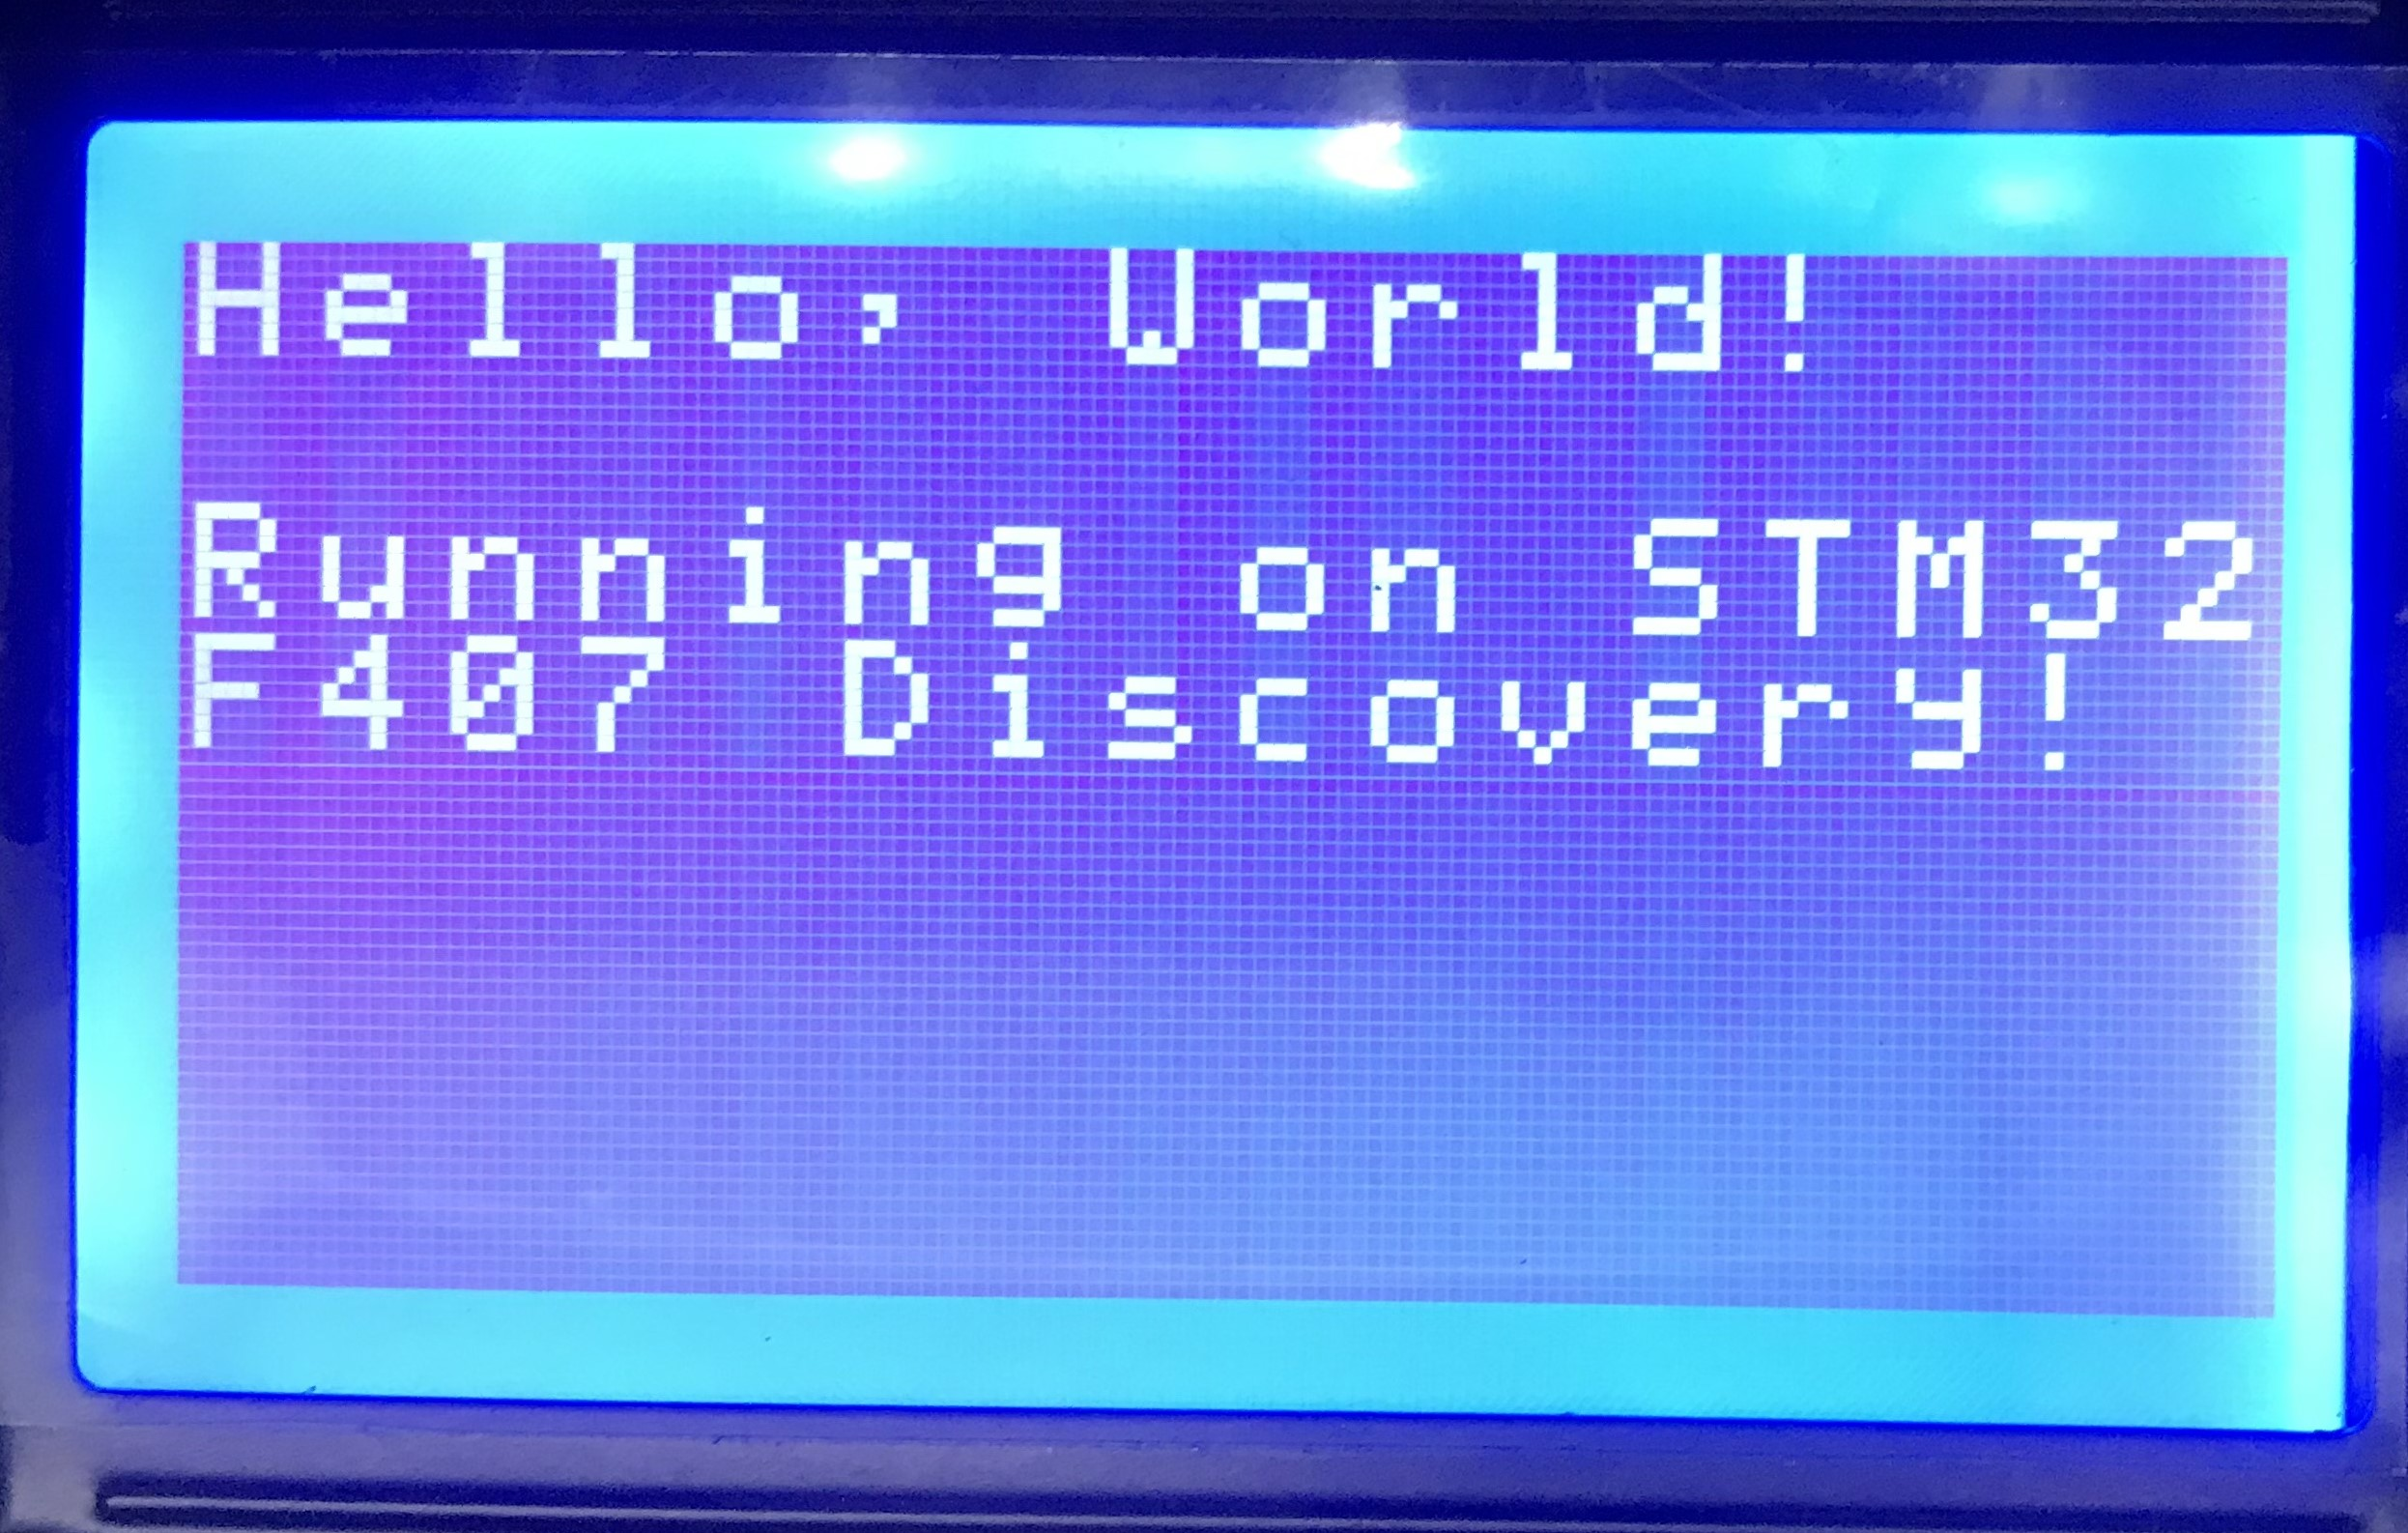
\includegraphics[width=.45\textwidth]{LCDScreens/helloworld.jpeg}} \qquad
    \subfloat[][HCMUT logo]{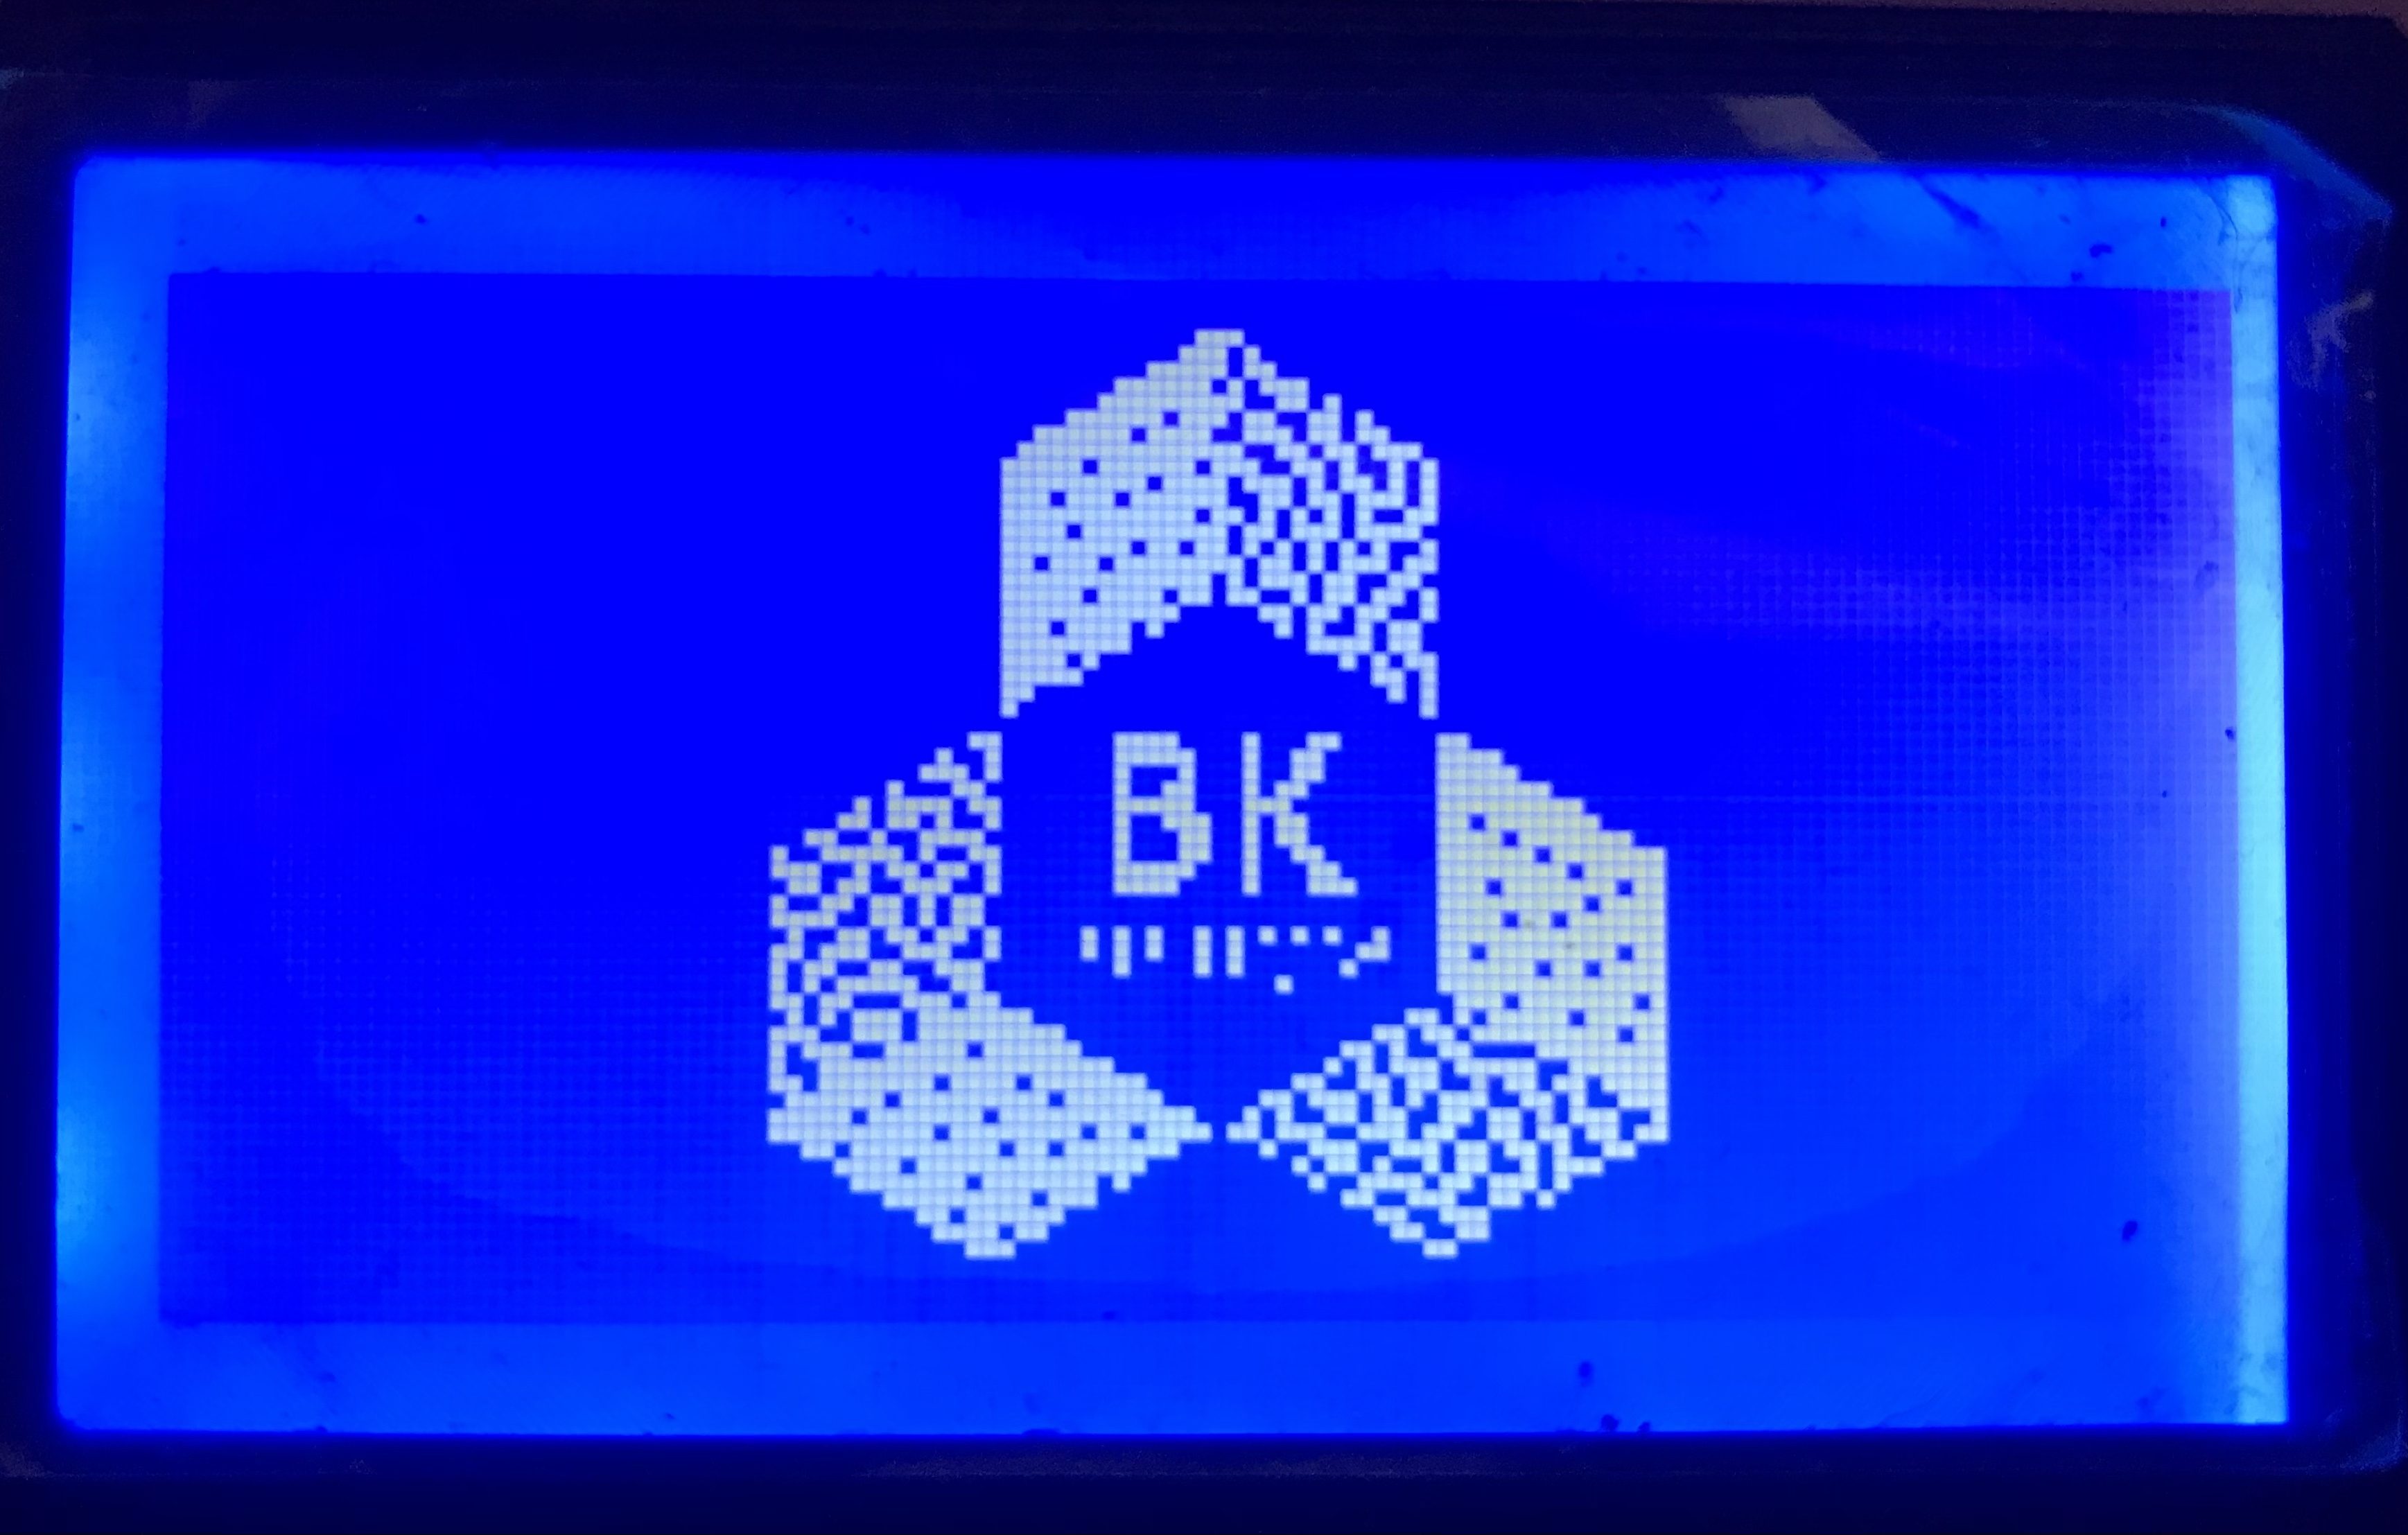
\includegraphics[width=.45\textwidth]{LCDScreens/logobk.jpeg}}
    \caption{LCD displaying text and bitmap image}
\end{figure}

\newpage
\section{Mathematical Evaluation}
\subsection{Key input buffer}
The provided code snippet introduces a custom enumeration called \texttt{Key}, which defines names for each button on the keypad instead of representing them as coordinates or text. This approach allows for easier interpretation and handling of button inputs. The enumeration includes a range of predefined names, such as \texttt{ZERO}, \texttt{ONE}, \texttt{TWO}, \texttt{THREE}, and so on, representing the corresponding buttons on the keypad. Additionally, it includes various mathematical operations like \texttt{PLUS}, \texttt{MINUS}, \texttt{MULTIPLY}, \texttt{DIVIDE}, as well as functions like \texttt{SQRT}, \texttt{SINE}, \texttt{COSINE}, and others. Furthermore, it encompasses special keys such as \texttt{BACKSPACE}, \texttt{BRACKET\_CLOSE}, \texttt{BRACKET\_OPEN}, and more. The enumeration also provides additional functionality, including navigation keys like \texttt{UP}, \texttt{DOWN}, \texttt{LEFT}, \texttt{RIGHT}, as well as utility keys like \texttt{AC} (All Clear) and \texttt{MODE}. This custom enumeration facilitates the mapping and processing of keypad inputs in a more intuitive and manageable manner. Each button pressed will returns the corresponding name.

\begin{code}
\captionof{listing}{Predefine names for each buttons}
\begin{minted}{C}
typedef enum {
  ZERO = 0, ONE = 1, TWO = 2, THREE = 3, FOUR = 4,
  FIVE = 5, SIX = 6, SEVEN = 7, EIGHT = 8, NINE = 9,
  DOT = 10, EQUAL = 11, ANSWER = 12,
  PLUS = 13, MINUS = 14, MULTIPLY = 15, DIVIDE = 16,
  EXPONENT = 17, XRT = 18, FACTORIAL = 19, BACKSPACE = 20,
  BRACKET_CLOSE = 21, BRACKET_OPEN = 22, SQRT = 23,
  SINE = 24, COSINE = 25, TANGENT = 26, COTANGENT = 27,
  LN = 28, LOG = 29, LOGX = 30, ABS = 31,

  COMMA = 48, S2D = 49,
  UP = 50, DOWN = 51, LEFT = 52, RIGHT = 53,
  AC = 54, EQUAL_SIGN = 55,
  LIMIT = 56, DERIVATIVE = 57, INTEGRAL = 58,

  X = 97, Y = 98, Z = 99,
  PINFTY = 133, NINFTY = 134,

  MODE = 253, TEST = 254
} Key;
\end{minted}
\end{code}

\subsection{Parsing key pressed array into a decimal number}
The goal of this is to convert an array of key presses, into a double-precision floating-point number. It handles both integer and decimal parts, supports negative numbers, and checks for various error conditions. The code iterates through the array, parsing the digits and constructing the resulting double value. If any errors occur during the parsing process, appropriate error codes are set, and the function returns NaN (Not a Number). Here is the flowchart for the algorithm:

\begin{figure}[H]
    \centering
    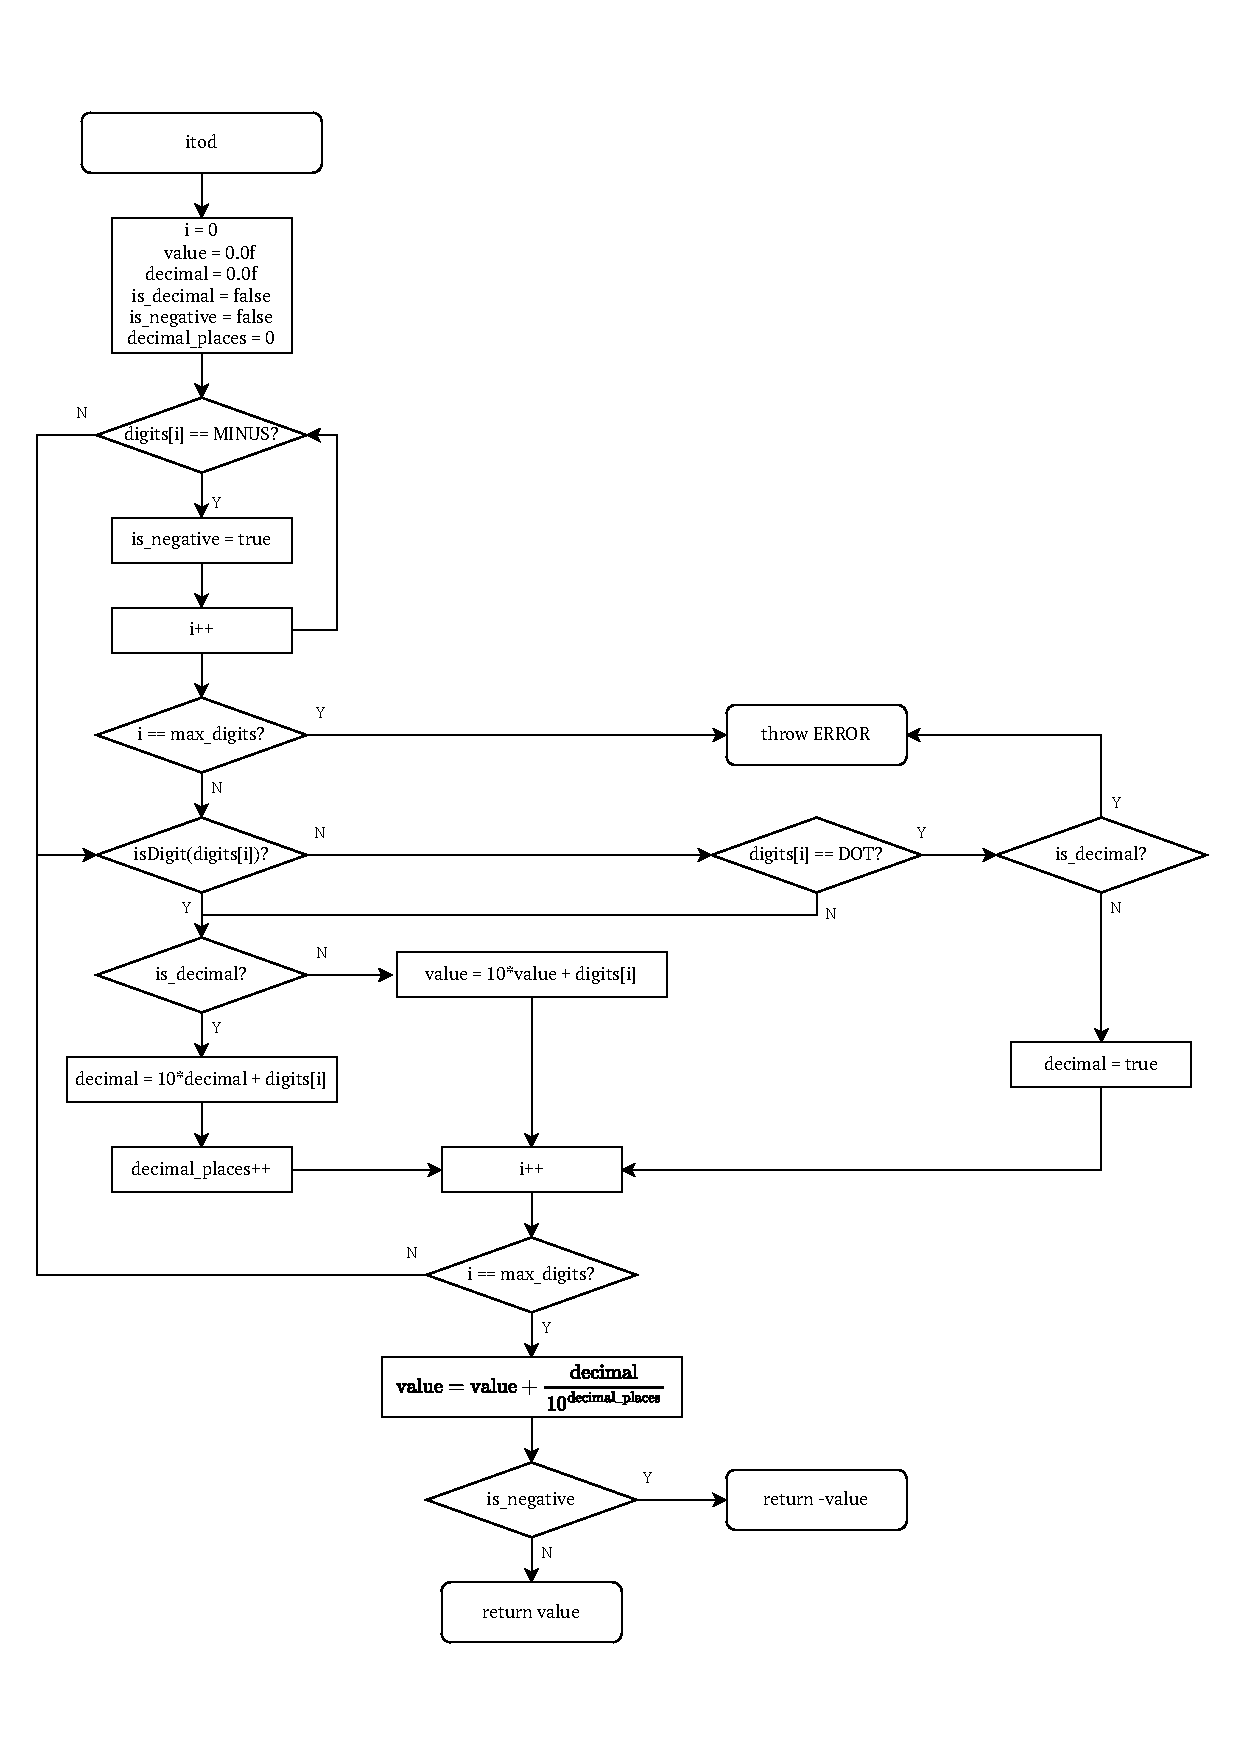
\includegraphics[height=.8\textheight, trim=0 1.5cm 0 1cm, clip]{images/itod.pdf}
    \caption{\texttt{itod} flowchart}
\end{figure}

\begin{code}
\captionof{listing}{Implemented C code for \texttt{itod}}
\begin{minted}{C}
double itod(const uint8_t * digits, uint8_t * errorCode, uint8_t * max_addr, int * endi) {
  double value = 0.0 f, decimal = 0.0 f;
  bool is_decimal = false, is_negative = false;
  uint8_t decimal_places = 0;

  int i = 0;

  // Check for minus sign
  while (digits[i] == MINUS) {
    is_negative = !is_negative;
    i++;
    if ((digits + i) == max_addr) {
      * errorCode = 1;
      return NAN;
    }
  }

  // Parse integer part
  while (digits[i] <= DOT && (digits + i) < max_addr) {
    if (digits[i] == DOT) {
      if (is_decimal) {
        * errorCode = 1;
        return NAN;
      }
      is_decimal = true;
      i++;
      continue;
    }
    if (is_decimal) {
      decimal = decimal * 10.0 f + digits[i];
      decimal_places++;
    } else {
      value = value * 10.0 f + digits[i];
    }
    i++;
  }

  * endi = i;

  // Calculate final value
  value += decimal / (double) pow(10.0 f, decimal_places);
  if (is_negative) return -value;
  return value;

  // Error: no digits found
  * endi = 0;
  return 0.0 f;
}
\end{minted}
\end{code}
The result, \texttt{errorCode}, \mintinline{c}{*maxAddr}, and \texttt{endi} are declared. \texttt{errorCode} is a byte to store the error code, \mintinline{c}{*maxAddr} is a pointer to the maximum address of the input array, and \texttt{endi} is an int to store the index of the last processed digit. The below code demonstrates the uses of \texttt{itod}.
\begin{minted}{c}
int main() {
    uint8_t input[5] = {MINUS, TWO, DOT, SIX, FIVE};
    uint8_t errorCode;
    uint8_t *maxAdrr = input+5;
    int endi;
    double result = itod(input, &errorCode, maxAdrr, &endi);
    printf("%g, %u, %d", result, errorCode, endi);
    return 0;
}
\end{minted}
And here is the result.
\begin{minted}{bash}
-2.65, 0, 5
\end{minted}

\subsection{Expression evaluation}
This is the hardest and the most important part of the software. We came up an idea, named ``Push-Pop Expression Evaluator''. Here's an overview of how it works:

\begin{enumerate}
    \item Initialize the necessary data structures: Before evaluating an expression, the evaluator initializes the operand and operator stacks, as well as any other required variables.
    \item Iterate over the expression: The evaluator goes through each character in the expression from left to right.
    \item Handle operands: If a character represents an operand (a number or a variable), it is pushed onto the operand stack.
    \item Handle operators: If a character represents an operator, the evaluator compares its precedence with the operator at the top of the operator stack. If the current operator has higher precedence or the operator stack is empty, the current operator is pushed onto the stack.
    \item Evaluate operators: If the current operator has lower precedence than the operator at the top of the stack, the evaluator pops the top operator and two operands from their respective stacks. The operation is performed on the operands using the operator, and the result is pushed back onto the operand stack.
    \item Continue evaluating operators: Steps 4 and 5 are repeated until the current operator has higher precedence than the operator at the top of the stack, or the stack is empty.
    \item Continue iterating over the expression: Steps 3 to 6 are repeated until all characters in the expression have been processed.
    \item Final evaluation: Once the expression has been fully processed, the evaluator checks if there are any remaining operators on the stack. If so, it pops the operator and two operands, performs the operation, and pushes the result back onto the operand stack.
    \item Return the result: After evaluating the expression, the final result is obtained by popping the top element from the operand stack.
\end{enumerate}

\subsubsection{Stack-based structure}
The stack is implemented as a LIFO (Last-In-First-Out) data structure, meaning that the last element inserted into the stack will be the first one to be removed. This property is essential for maintaining the correct order of operands and operators during expression evaluation.

The stack structure consists of an array to hold the elements of the stack and a top variable to keep track of the index of the topmost element in the stack.

The stack structure allows for efficient insertion and removal of elements, with a constant time complexity of O(1). It is utilized in the expression evaluator to store operands and operators during the evaluation process.

\begin{minted}{c}
struct stack {
	int top;
	double items[MAX];
};
\end{minted}

By using the stack structure, the evaluator can correctly handle nested expressions and maintain the order of operations. The operands and operators are pushed onto the stack as they are encountered in the expression, and the necessary operations are performed by popping the elements from the stack in the appropriate order.

To push an item onto the stack, the top variable is incremented, and the item is stored at the corresponding index in the items array. This operation effectively adds a new element to the top of the stack.

To pop an item from the stack, the item at the current top index is retrieved, and the top variable is decremented. This operation removes the topmost element from the stack.

\begin{minted}{c}
void push(struct stack *s, double value, uint8_t *error) {
    if (s->top == MAX - 1) {
        // Stack is full
        *error = 1;
        return;
    }
    s->items[++(s->top)] = value;
}
double pop(struct stack *s, uint8_t *error) {
    if (s->top == -1) {
        // Stack is empty
        *error = 2;
        return 0;
    }
    return s->items[(s->top)--];
}
\end{minted}

By using the push and pop operations on the operand and operator stacks, the evaluator ensures that the expression is evaluated based on the correct order of operations and operator precedence. This stack-based approach allows for the evaluation of complex mathematical expressions.

\subsubsection{Determine if a character is an operator}
The `\texttt{is\_operator}` function takes a character as input and returns an integer value indicating whether the character corresponds to one of the supported operators in the expression evaluator. The function uses a series of logical OR operators to compare the input character (`c`) against predefined constants representing various operators such as `\texttt{PLUS}`, `\texttt{MINUS}`, `\texttt{MULTIPLY}`, `\texttt{DIVIDE}`, `\texttt{EXPONENT}`, `\texttt{SQRT}`, `\texttt{XRT}`, `\texttt{FACTORIAL}`, `\texttt{SINE}`, `\texttt{COSINE}`, `\texttt{TANGENT}`, `\texttt{LN}`, `\texttt{LOG}`, `\texttt{LOGX}`, and `\texttt{ABS}`. If the input character matches any of these operators, the function returns \mintinline{c}{true}, indicating that it is indeed an operator. Otherwise, it returns \mintinline{c}{false}, indicating that the character is not an operator.
\begin{minted}{c}
bool is_operator(char c) {
    return c == PLUS || c == MINUS || c == MULTIPLY || c == DIVIDE ||
           c == EXPONENT || c == SQRT || c == XRT || c == FACTORIAL ||
           c == SINE || c == COSINE || c == TANGENT || c == LN || c == LOG ||
           c == LOGX ||  c == ABS;
}
\end{minted}

\subsubsection{Determine if the operator requires only one argument}

The function takes an operator \texttt{op} as input and returns a boolean value indicating whether the operator is a one-argument operator.

In the function, a series of logical OR operators (\texttt{||}) are used to check if the given operator matches any of the predefined one-argument operators (\texttt{SQRT}, \texttt{SINE}, \texttt{COSINE}, \texttt{TANGENT}, \texttt{LN}, \texttt{LOG}, \texttt{FACTORIAL}, \texttt{ABS}). 

If the operator matches any of these operators, the function will return \mintinline{c}{true}, indicating that it is a one-argument operator. Otherwise, it will return \mintinline{c}{true}, indicating that it is not a one-argument operator.

\begin{minted}{c}
bool isOneArgOperator(char op) {
	return op == SQRT || op == SINE || op == COSINE || op == TANGENT ||
	       op == LN || op == LOG || op == FACTORIAL || op == ABS;
}
\end{minted}

\subsubsection{Determine if a character is a variable}
The `\texttt{is\_variable}` function is similar to `\texttt{is\_operator}`, but it is used to determine whether a given character corresponds to a variable. The function compares the input character against predefined constants representing variables such as `\texttt{ANSWER}`, `\texttt{X}`, `\texttt{Y}`, and `\texttt{Z}`. If the input character matches any of these variables, the function returns \mintinline{c}{true}, indicating that it is a variable. Otherwise, it returns \mintinline{c}{false}, indicating that the character is not a variable.
\begin{minted}{c}
bool is_variable(char c) {
	return c == ANSWER || c == X || c == Y || c == Z;
}
\end{minted}

\subsubsection{Operator precedence}
The operators are categorized into different precedence levels, with higher precedence values indicating higher priority. Here is a breakdown of the precedence levels assigned to each operator:

\begin{itemize}
    \item Operators with precedence 5: \texttt{SQRT}, \texttt{SINE}, \texttt{COSINE}, \texttt{TANGENT}, \texttt{LN}, \texttt{LOG}, \texttt{LOGX}, \texttt{ABS}
    \item Operator with precedence 4: \texttt{FACTORIAL}
    \item Operators with precedence 3: \texttt{EXPONENT}, \texttt{XRT}
    \item Operators with precedence 2: \texttt{MULTIPLY}, \texttt{DIVIDE}
    \item Operators with precedence 1: \texttt{PLUS}, \texttt{MINUS}
    \item Default case (no match): returns 0
\end{itemize}

\begin{minted}{c}
uint8_t precedence(char op) {
  switch (op) {
    case SQRT:
    case SINE:
    case COSINE:
    case TANGENT:
    case LN:
    case LOG:
    case LOGX:
    case ABS:
      return 5;
    case FACTORIAL:
      return 4;
    case EXPONENT:
    case XRT:
      return 3;
    case MULTIPLY:
    case DIVIDE:
      return 2;
    case PLUS:
    case MINUS:
      return 1;
    default:
      return 0;
  }
}
\end{minted}

By assigning precedence values to operators, this function helps in determining the order of operations when evaluating an expression. Operators with higher precedence will be evaluated first before operators with lower precedence, ensuring the correct calculation order in the expression evaluation process.

\subsubsection{Perform calculations}
The function performs the arithmetic or mathematical operation specified by the operator (\texttt{op}) on the given operands (\texttt{x} and \texttt{y}). The function also takes a pointer to an \texttt{uint8\_t} variable called \texttt{error} as input, which is used to track any errors that occur during the operation.

Here is a breakdown of the operations performed for each case:

\begin{itemize}
    \item Addition (\texttt{PLUS}): Returns $x+y$.
    \item Subtraction (\texttt{MINUS}): Returns $x-y$.
    \item Multiplication (\texttt{MULTIPLY}): Returns $x\times y$.
    \item Division (\texttt{DIVIDE}): If \texttt{y} is not zero, returns $x\div y$. If \texttt{y} is zero, sets \texttt{error} to 4 (indicating division by zero error) and returns \texttt{NAN} (not-a-number).
    \item Exponentiation (\texttt{EXPONENT}): Returns $x^y$.
    \item Square root (\texttt{SQRT}): Returns the $\sqrt x$.
    \item Nth root (\texttt{XRT}): Returns $\sqrt[x] y$.
    \item Sine (\texttt{SINE}): Returns $\sin x$.
    \item Cosine (\texttt{COSINE}): Returns $\cos x$.
    \item Tangent (\texttt{TANGENT}): Returns $\tan x$.
    \item Natural logarithm (\texttt{LN}): Returns $\ln x$.
    \item Logarithm (\texttt{LOG}): Returns $\log x = \log_{10} x$.
    \item Logarithm with custom base (\texttt{LOGX}): Returns $\log_x y$.
    \item Factorial (\texttt{FACTORIAL}): Returns $x! = \Gamma(x+1)$.
    \item Absolute value (\texttt{ABS}): Returns $|x|$.
\end{itemize}

If the operator character doesn't match any of the cases, indicating an invalid operator, the function returns 0.

The function also handles the special case of division by zero by setting the error code to 4 and returning NaN. The error code is updated only if it is greater than 2 or equal to 0, allowing for the possibility of tracking multiple errors.

These are operators that we implemented till now, there are some operators we will add in the future such as inverse and hyperbolic sine/cosine/tangent, etc.

\begin{minted}{c}
double operate(double x, double y, char op, uint8_t * error) {
  switch (op) {
  case PLUS:
    return x + y;
  case MINUS:
    return x - y;
  case MULTIPLY:
    return x * y;
  case DIVIDE:
    if (y == 0) {
      // Division by zero
      if ( * error > 2 || * error == 0) * error = 4;
      return NAN;
    }
    return x / y;
  case EXPONENT:
    return pow(x, y);
  case SQRT:
    return sqrt(x);
  case XRT:
    return pow(y, 1.0 / x);
  case SINE:
    return sin(x);
  case COSINE:
    return cos(x);
  case TANGENT:
    return tan(x);
  case LN:
    return log10(x) / log10(E);
  case LOG:
    return log10(x);
  case LOGX:
    return log10(y) / log10(x);
  case FACTORIAL:
    return tgamma(x + 1);
  case ABS:
    return fabs(x);
  default:
    // Invalid operator
    return 0;
  }
}
\end{minted}

\subsubsection{Pop -- Calculate -- Push}
We call this a ``Pop -- Calculate -- Push'' (PCP) process, since it is sequence of steps used to evaluate an expression using stacks. It involves retrieving operators and operands from their respective stacks, performing the necessary calculation, and pushing the result back onto the operands stack. Here's how the process works:

\begin{enumerate}
    \item Pop: The first step is to pop operand(s) and one operator from their respective stacks. The operands represent the values on which the operator will operate, and the operator specifies the type of operation to be performed.
    \item Calculate: Once the operand(s) and operator are obtained, the next step is to perform the calculation. The \texttt{operate} function is called with the operands and operator as arguments. This function applies the appropriate operation to the operands and returns the result.
    \item Push: After the calculation is performed, the result is pushed back onto the operands stack. This ensures that the result is available for subsequent calculations.
\end{enumerate}

\begin{minted}{c}
void calculate(struct stack * operators, struct stack * operands, uint8_t * errorCode) {
  // pop operand(s) and one operator
  char op = pop(operators, errorCode);
  double y = 0;
  if (!isOneArgOperator(op))
    y = pop(operands, errorCode);
  double x = pop(operands, errorCode);

  // evaluate the expression x op y and push the result into operands stack
  push(operands, operate(x, y, op, errorCode), errorCode);
}
\end{minted}

By repeating the ``Pop -- Calculate -- Push'' (PCP) process iteratively, the expression is evaluated step by step until all operators have been processed and the final result remains in the operands stack. The process continues until the expression is fully evaluated.

\subsubsection{Expression Evaluation}
Based on the idea that has discussed at the beginning, here is the pseudo code for the function:
\begin{minted}{python}
function ExpEvaluate(exp, size):
  initialize operands stack
  initialize operators stack
  initialize numOpenBrackets and numCloseBrackets to 0

  for i = 0 to size-1:
    if exp[i] is a digit, decimal point, or negative sign:
      value = parse the number
      push value into operands stack
      
      if i is not the last index and the next character is not a closing bracket or a comma:
        push MULTIPLY into operators stack
    
    else if exp[i] is PINFTY:
      push positive infinity into operands stack
    
    else if exp[i] is NINFTY:
      push negative infinity into operands stack
    
    else if exp[i] is a minus sign and (i is 0 or the previous character is an opening bracket or an operator):
      push 0 into operands stack
      push MINUS into operators stack
    
    else if exp[i] is a variable:
      push the value of the variable into operands stack
      
      if i is not the last index and the next character is not a closing bracket or a comma:
        push MULTIPLY into operators stack
    
    else if exp[i] is an opening bracket:
      push exp[i] into operators stack
      increment numOpenBrackets by 1
    
    else if exp[i] is a closing bracket:
      while operators stack is not empty and the top of the stack is not an opening bracket:
        evaluate by PCP
      
      if operators stack is not empty:
        pop the top of the stack (opening bracket)
      else:
        throw error for bracket mismatch
      
      if i is not the last index and the next character is not a closing bracket or a comma:
        push MULTIPLY into operators stack
      
      increment numCloseBrackets by 1
    
    else if exp[i] is a comma:
      while operators stack is not empty and the top of the stack is not an opening bracket:
        evaluate by PCP
    
    else if exp[i] is an operator:
      if exp[i] is FACTORIAL and the next character is a digit or decimal point:
        throw error for syntax error
      
      while operators stack is not empty and the precedence of the top operator is greater than or equal to the precedence of exp[i]:
        evaluate by PCP
      
      push exp[i] into operators stack
    
    else:
      throw error for invalid character
  
  if numOpenBrackets is not equal to numCloseBrackets:
    throw error for bracket mismatch
  
  while operators stack is not empty:
    evaluate by PCP
  
  if operands stack has more than one value:
    throw error for bug
  
  answer = pop the top value from operands stack
  store answer in a variable named ANSWER
  
  return answer
\end{minted}

The function takes in an expression and its size as input and evaluates the expression using the operator precedence rules. It uses two stacks, one for operands and another for operators, to store and process the values and operations in the expression. The function iterates through each character in the expression, handling digits, variables, operators, brackets, and commas according to the specified rules. It performs calculations and pushes the results onto the operands stack until the entire expression is evaluated. Finally, it returns the computed result and stores it in a variable \texttt{ANSWER}.

Below is the C code implementation. The function below has a checking process for the calculus operators (find limit, taking derivative and integration) which we will discuss later.

\begin{minted}{c}
double ExpEvaluate(uint8_t * exp, uint8_t size, uint8_t * errorCode) {
  // Clear errors
  * errorCode = 0;

  // create two stacks: one for operands and one for operators
  struct stack operands = { -1 };
  struct stack operators = { -1 };

  // track the number of opening and closing parentheses
  int numOpenBrackets = 0;
  int numCloseBrackets = 0;

  // loop through each character in the expression
  for (int i = 0; i < size; i++) {
    if (exp[i] == DERIVATIVE || exp[i] == LIMIT || exp[i] == INTEGRAL) {
      char mode = exp[i];
      // Find the comma
      int j, arg0Size = 0, arg1Size = 0, arg2Size = 0;
      for (j = i + 2; j < size; j++) {
        if (exp[j] == BRACKET_OPEN)
          numOpenBrackets++;
        else if (exp[j] == BRACKET_CLOSE)
          numCloseBrackets++;

        if (exp[j] == COMMA && numOpenBrackets == numCloseBrackets) {
          if (arg0Size == 0) {
            arg0Size = j - i - 2;
          } else { // arg1Size
            arg1Size = j - i - 2 - arg0Size - 1;
          }
        } else if (exp[j + 1] == BRACKET_CLOSE && numOpenBrackets == numCloseBrackets) {
          if (arg1Size == 0)
            arg1Size = j - i - 2 - arg0Size;
          else
            arg2Size = j - i - 2 - arg0Size - arg1Size - 1;
          break;
        }
      }

      if (mode == DERIVATIVE || mode == LIMIT) {
        if (arg0Size == 0 || arg1Size == 0 || arg2Size > 0) {
          * errorCode = 1;
          return NAN;
        }
      } else if (mode == INTEGRAL) {
        if (arg0Size == 0 || arg1Size == 0 || arg2Size == 0) {
          * errorCode = 1;
          return NAN;
        }
      }

      double x0 = ExpEvaluate(exp + arg0Size + i + 3, arg1Size, errorCode);

      double result = 0;
      if (mode == DERIVATIVE) {
        result = derivative(exp + i + 2, x0, arg0Size, errorCode);
        i += arg0Size + arg1Size + 3;
      } else if (mode == LIMIT) {
        result = limit(exp + i + 2, x0, arg0Size, errorCode);
        i += arg0Size + arg1Size + 3;
      } else if (mode == INTEGRAL) {
        double x1 = ExpEvaluate(exp + arg0Size + arg1Size + i + 4, arg2Size, errorCode);
        result = integrate(exp + i + 2, x0, x1, TOLERANCE, 25, arg0Size, errorCode);
        i += arg0Size + arg1Size + arg2Size + 4;
      }

      push( & operands, result, errorCode);
    }
    // if the character is a digit or a decimal point or a negative sign,
    // read the whole number and push it into operands stack
    else if (exp[i] <= DOT || (exp[i] == MINUS && exp[i + 1] <= DOT &&
        (i == 0 || exp[i - 1] == BRACKET_OPEN || is_operator(exp[i - 1]))
      )) {

      int endi;
      double value = itod( & exp[i], errorCode, exp + size, & endi);

      if (exp[endi + 1] == DOT && exp[endi + 2] > NINE) { // after DOT must be a number
        * errorCode = 1;
        return 0;
      }

      i += endi - 1;

      // push the value into operands stack
      push( & operands, value, errorCode);

      // check if not the last digit, append *
      if (i < size - 1 && (exp[i + 1] > BRACKET_CLOSE || exp[i + 1] == ANSWER) && exp[i + 1] != COMMA)
        push( & operators, MULTIPLY, errorCode);
    } else if (exp[i] == PINFTY) {
      push( & operands, DBL_MAX, errorCode);
    } else if (exp[i] == NINFTY) {
      push( & operands, -DBL_MAX, errorCode);
    } else if (exp[i] == MINUS &&
      (i == 0 || exp[i - 1] == BRACKET_OPEN || is_operator(exp[i - 1]))) {
      push( & operands, 0, errorCode);
      push( & operators, MINUS, errorCode);
    } else if (is_variable(exp[i])) {
      push( & operands, GetVar(exp[i]), errorCode);
      if (i < size - 1 && (exp[i + 1] > BRACKET_CLOSE || exp[i + 1] == ANSWER) && exp[i + 1] != COMMA)
        push( & operators, MULTIPLY, errorCode);
    }
    // if the character is an opening parenthesis,
    // push it into operators stack
    else if (exp[i] == BRACKET_OPEN) {
      push( & operators, exp[i], errorCode);
      numOpenBrackets++;
    }

    // if the character is a closing parenthesis,
    // pop and evaluate all operators until an opening parenthesis is found
    else if (exp[i] == BRACKET_CLOSE) {
      while (operators.top != -1 && operators.items[operators.top] != BRACKET_OPEN) {
        calculate( & operators, & operands, errorCode);
      }

      // pop and discard the opening parenthesis
      if (operators.top != -1) {
        pop( & operators, errorCode);
      } else {
        * errorCode = 3;
        return 0;
      }

      if (i < size && (exp[i + 1] > BRACKET_CLOSE || exp[i + 1] == ANSWER) && exp[i + 1] != COMMA)
        push( & operators, MULTIPLY, errorCode);
      numCloseBrackets++;
    }

    // if the character is a comma,
    else if (exp[i] == COMMA) {
      while (operators.top != -1 && operators.items[operators.top] != BRACKET_OPEN) {
        calculate( & operators, & operands, errorCode);
      }
    }

    // if the character is an operator,
    // pop and evaluate all operators with higher or equal precedence
    else if (is_operator(exp[i])) {
      // Shouldn't any number after FACTORIAL
      if (exp[i] == FACTORIAL && i < size - 1 && exp[i + 1] <= DOT) {
        * errorCode = 1;
        return 0;
      }
      while (operators.top != -1 && precedence(operators.items[operators.top]) >= precedence(exp[i])) {
        calculate( & operators, & operands, errorCode);
      }

      // push the current operator into operators stack
      push( & operators, exp[i], errorCode);
    }

    // if the character is invalid, print an error message and exit
    else {
      // Invalid character
    }
  }

  if (numCloseBrackets != numOpenBrackets) {
    * errorCode = 3;
    return 0;
  }

  // pop and evaluate all remaining operators
  while (operators.top != -1) {
    calculate( & operators, & operands, errorCode);
  }

  // the final result is the only value left in operands stack
  if (operands.top > 0)
    *
    errorCode = 1;

  answer = pop( & operands, errorCode);
  if ( * errorCode == 0)
    SetVar(ANSWER, answer);
  return answer;
}
\end{minted}

\subsubsection{Demonstration and test cases}
By implementing all the previously discussed code, we have successfully developed a functional evaluation system. With this system, we can perform basic mathematical evaluations by parsing and processing expressions. Now, we can proceed to demonstrate the functionality of the evaluation system by showcasing a demo and executing various test cases. These test cases will cover a range of mathematical operations and expressions to ensure the accuracy and reliability of the evaluation system. Through this demonstration, we can validate the effectiveness of the implemented code and its ability to handle different scenarios in mathematical evaluation.

\begin{minted}{c}
int main() {
    char inputs[50] = {TWO, PLUS, FIVE, DIVIDE, NINE};
	uint8_t errorCode = 0;
	double answer = evaluate(inputs, 5, &errorCode);
	printf("%0.10f, %d\n", answer, errorCode);
    return 0;
}
\end{minted}

\begin{minted}{c}
// 2 + 5 / 9
inputs = {TWO, PLUS, FIVE, DIVIDE, NINE} 
result: 2.5555555556, 0

// 2 / 0
inputs = {TWO, DIVIDE, ZERO} 
result: nan, 4

// 1.2 (3.45 + 6) / 7.8 ^ 9
inputs = {ONE, DOT, TWO, BRACKET_OPEN, THREE, DOT, FOUR, FIVE, PLUS, SIX, BRACKET_CLOSE, DIVIDE, SEVEN, DOT, EIGHT, EXPONENT, NINE}
result: 0.0000001061, 0

// sqrt(729) + log2(512) - cos(0) = 27 + 9 - 1 = 35
inputs = {SQRT, SEVEN, TWO, NINE, PLUS, LOGX, BRACKET_OPEN, TWO, COMMA, FIVE, ONE, TWO, BRACKET_CLOSE, MINUS, COSINE, ZERO}
result: 35.0000000000, 0
\end{minted}

\subsection{Calculus and other operations}
In addition to the basic mathematical operations, our evaluation system also supports calculus operators, expanding its functionality to include more advanced mathematical concepts. These calculus operators allow users to find limits, differentiate functions, and perform integrations. By incorporating these capabilities, our system provides a comprehensive tool for mathematical analysis and problem-solving. Whether it's evaluating complex expressions or tackling calculus-related tasks, users can rely on our system to handle a wide range of mathematical operations effectively and accurately.

When it comes to finding limits, our evaluation system employs an approximation method. This method enables users to determine the behavior of a function as it approaches a particular value or approaches infinity. By utilizing this approximation technique, users can obtain valuable insights into the behavior of mathematical functions without relying on exact calculations.

For differentiation, our system utilizes the central difference formula. This numerical approximation method allows users to compute the derivative of a function at a given point. By estimating the slope of the function at the point of interest using nearby points, the central difference formula provides an efficient way to approximate derivatives and explore the rate of change of functions.

In terms of integration, our system leverages the adaptive Simpson's rule. This numerical integration technique divides the integration interval into smaller segments and approximates the area under the curve by employing a combination of quadratic approximations. By adaptively adjusting the segment sizes based on the local behavior of the function, the adaptive Simpson's rule offers an accurate approximation of integrals and enables users to compute definite integrals more efficiently.

By incorporating these approximation methods and numerical techniques, our evaluation system empowers users to explore the realms of calculus, enabling them to find limits, compute derivatives, and perform integrations with confidence and accuracy.

In this report, we would like to clarify that the implementation details of the approximation method for finding limits, the central difference formula for differentiation, and the adaptive Simpson's rule for integration are beyond the scope of our current discussion. However, for those interested in delving into the technical aspects of these functionalities, we have included the relevant source code in the appendix section of our report. This allows readers to explore the intricacies of these numerical methods and gain a deeper understanding of the algorithms employed in our calculator's advanced calculus capabilities.

\section{Graphical Interface}
Currently, Our scientific calculator featuring two modes: math mode and graphing mode. In math mode, users can input mathematical expressions and obtain precise numerical results. The calculator evaluates the expressions, handles basic arithmetic operations, and supports advanced mathematical functions like logarithms, exponentials, and trigonometric functions. On the other hand, graphing mode allows users to visualize mathematical functions by plotting them on a graphical display. By selecting the desired mode, users can seamlessly switch between performing calculations and graphing functions, thereby enhancing the calculator's utility and versatility.

\subsection{Select Mode Menu}
This function allows the user to choose between two modes: Math Mode and Graphing Mode. The menu is displayed on a graphical LCD screen and consists of two options: \texttt{Math Mode} and \texttt{Graphing Mode}. Initially, the current mode is highlighted as the selected row. The user can navigate through the menu options using the arrow keys, moving the selection up or down. Pressing the \texttt{EQUAL} key confirms the selection and returns the chosen mode. Alternatively, pressing the \texttt{AC} key cancels the selection and returns the current mode. The function ensures that the selected row is visually distinguished by toggling its appearance on the screen, providing a clear and interactive menu interface.
\begin{minted}{c}
uint8_t maxRow = 1;

uint8_t SelectModeMenu() {
  uint8_t selectedRow = currentMode;
  GLCD_Buf_Clear();
  GLCD_Font_Print(0, 0, "Math Mode");
  GLCD_Font_Print(0, 1, "Graphing Mode");

  ToggleRow(selectedRow);
  ST7920_Update();

  while (1) {
    uint8_t key = KeyPad_WaitForKeyGetChar(0, false);
    if (key != 0xFF) {
      if (key == DOWN && selectedRow < maxRow) {
        ToggleRow(selectedRow);
        selectedRow++;
        ToggleRow(selectedRow);
      } else if (key == UP && selectedRow > 0) {
        ToggleRow(selectedRow);
        selectedRow--;
        ToggleRow(selectedRow);
      } else if (key == EQUAL) {
        return selectedRow;
      } else if (key == AC) {
        return currentMode;
      } else continue;

      ST7920_Update();
    }
  }
}
\end{minted}
\begin{figure}[H]
    \centering
    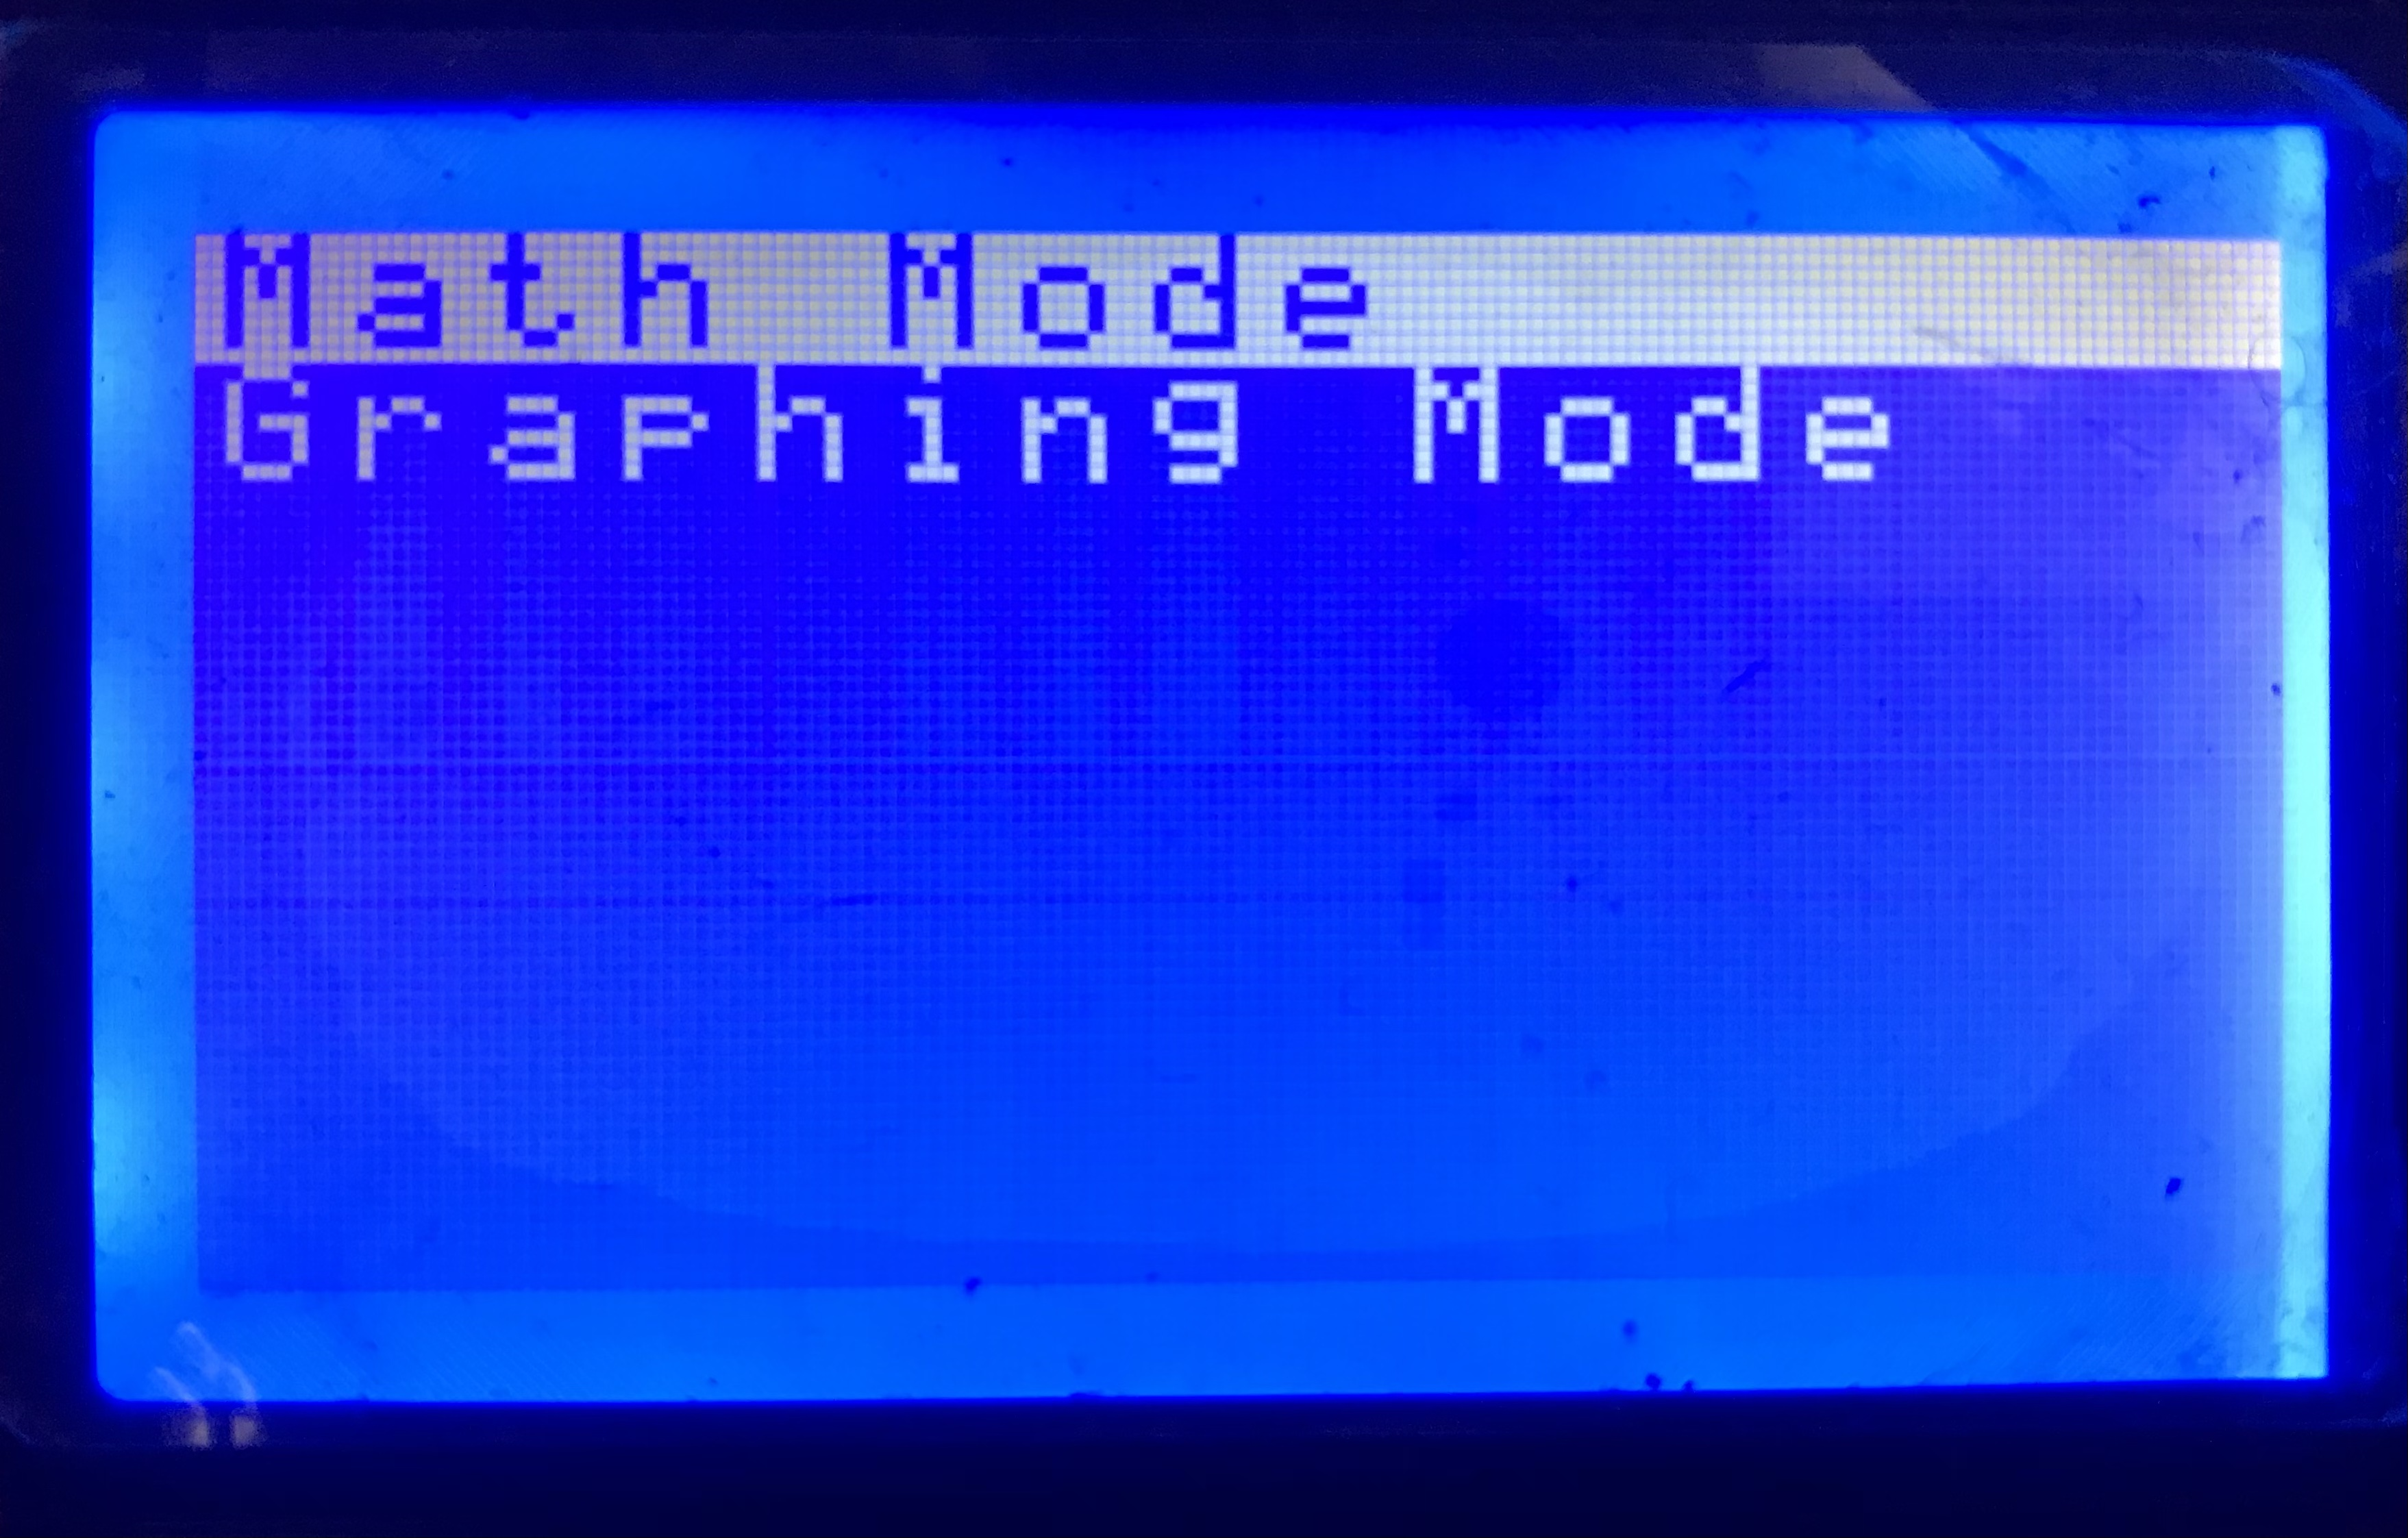
\includegraphics[width=.7\textwidth]{LCDScreens/menu.jpeg}
    \caption{Menu screen}
\end{figure}

\subsection{Math Mode}
The graphical interface of the system consists of two sections: the user input area and the result display. The user input area occupies the rows from 0 to 6, providing ample space for entering mathematical expressions and equations. The user can navigate within the input area using a cursor, which can be moved using the left and right buttons. This allows for easy editing and modification of the input. The result display is located in the last row (row 7) and shows the output of the mathematical computations performed based on the user's input. 
To facilitate the functionality described above, the system employs two buffers: an input buffer and a display buffer. The input buffer is responsible for storing the user's input, which includes mathematical expressions and equations. This buffer holds the entire input string as defined earlier. The display buffer, on the other hand, is used to show the individual characters of the input string. For example, if the input is \texttt{SINE} the display buffer would show \texttt{s i n} separately. The display buffer updates and refreshes whenever a button is clicked, allowing the user to see their input characters one by one as they navigate through the input area using the cursor. This implementation enhances the user experience by providing real-time feedback and visualizing the input in a clear and readable manner.

Additionally, the system incorporates two counters: the length counter and the current cursor position counter. Both counters are initialized to zero. The length counter keeps track of the length of the input string, incrementing by one each time a new character is entered. Similarly, the current cursor position counter is incremented by one when a character is added, indicating the current position of the cursor within the input string. 

When the user presses the left or right button to navigate through the input, the current cursor position is either incremented or decremented accordingly. However, to ensure that the cursor stays within the valid range of 0 to the length of the input string, the current cursor position is clamped, preventing it from going below 0 or exceeding the length. This clamping mechanism guarantees that the cursor always remains within the bounds of the available input characters, providing a smooth and user-friendly experience.

To implement a blinking cursor in our program, we us a timer interrupt to toggle the visibility of the cursor at 500 miliseconds intervals. Just configurate the timer as same as the microsecond timer that we discuss earlier, and change the prescaler to 3200-1 and counter period to 5000. Then write a callback function for timer interrupt to toggle the cursor every 500 miliseconds.

\begin{minted}{c}
void HAL_TIM_PeriodElapsedCallback(TIM_HandleTypeDef *htim) {
  if (htim->Instance == TIM2) {
    ToggleCursor();
    ST7920_Update();
  }
}
\end{minted}

\mintinline{c}{ToggleCursor()} and \mintinline{c}{ToggleCursorOnOff(bool isOn)}: These functions toggle the visibility of the cursor on the display. \mintinline{c}{ToggleCursor()} toggles the cursor state, while \mintinline{c}{ToggleCursorOnOff(bool isOn)} allows explicitly setting the cursor state.
\begin{minted}{c}
void ToggleCursor() {
  cursorState = !cursorState;
  ToggleRectangle(disX * 8, disY * 8, 1, 6);
}
void ToggleCursorOnOff(bool isOn) {
  cursorState = isOn;
  if(isOn)
    ToggleRectangle(disX * 8, disY * 8, 1, 6);
}
\end{minted}

Now we discuss several functions related to the graphical interface and input handling.

\mintinline{c}{GetChar(uint8_t ch)}: This function returns the character representation of the given input \mintinline{c}{ch}. It handles various special characters and mathematical symbols and returns their corresponding character representation.
\begin{minted}{c}
char * GetChar(uint8_t ch) {
    if (ch < 10) {
      static char c[] = {0, 0};
      c[0] = ch + 48;
      return c;
    } else if (ch == LN) {
      static char c[] = {'l', 'n', 0};
      return c;
    } else if (ch == DERIVATIVE) {
      static char c[] = {'d', '(', 0};
      return c;
      // ...
    } else if (ch == SINE || ch == COSINE || ch == TANGENT || ch == ANSWER ||
      ch == LOG || ch == ABS) {
      static char c[] = {0, 0, 0, 0};
      switch (ch) {
      case SINE:
        c[0] = 's';
        c[1] = 'i';
        c[2] = 'n';
        break;
        // ...
      case ABS:
        c[0] = 'a';
        c[1] = 'b';
        c[2] = 's';
        break;
      }
      return c;
    } else if (ch == LOGX) {
      static char c[] = {'l', 'o', 'g', '(', 0};
      return c;
    } else {
      static char c[] = {0, 0};
      switch (ch) {
      case DOT:
        c[0] = '.';
        break;
      case PLUS:
        c[0] = '+';
        break;
      case MINUS:
        c[0] = '-';
        break;
        // ...
        return c;
      }
    }
\end{minted}

\mintinline{c}{UpdateCursor()}: This function updates the cursor position based on the current input. It calculates the cursor's X and Y coordinates on the display by iterating through the input characters and accumulating the character lengths.
\begin{minted}{c}
void UpdateCursor() {
    disX = 0;
    for (int i = 0; i < input_ptr; i++)
      disX += charLength[i];

    disY = disX / 16;
    disX = disX % 16;
}
\end{minted}

\mintinline{c}{UpdateDisp()}: This function updates the display buffer with the formatted input string. It iterates through the input characters, converts them to their corresponding characters using \mintinline{c}{GetChar()}, and appends them to the display buffer. It also updates the \mintinline{c}{charLength} array, which stores the length of each character in the input.
\begin{minted}{c}
void UpdateDisp() {
  disp_buff[0] = '\0';
  for (int i = 0; i < input_length; i++) {
    if (input[i] == BRACKET_OPEN &&
      (input[i - 1] == LOGX || input[i - 1] == DERIVATIVE ||
        input[i - 1] == LIMIT || input[i - 1] == INTEGRAL)) {
      charLength[i] = 0;
    } else {
      char * c = GetChar(input[i]);
      strcat(disp_buff, c);
      charLength[i] = strlen(c);
    }
  }
  strcat(disp_buff, "     ");

  GLCD_Font_Print(0, 0, disp_buff);
  ST7920_Update();
  UpdateCursor();
}
\end{minted}

\mintinline{c}{AddKey(uint8_t key)}: This function adds a key to the input string. It handles special cases when certain keys (e.g., \mintinline{c}{LOGX}, \mintinline{c}{DERIVATIVE}, \mintinline{c}{LIMIT}, \mintinline{c}{INTEGRAL}) are pressed, inserting additional characters into the input string.
\begin{minted}{c}
void AddKey(uint8_t key) {
  if (key == LOGX || key == DERIVATIVE || key == LIMIT || key == INTEGRAL) {
    input_length += 2;
    for (int i = input_length - 1; i >= input_ptr + 2; i--) {
      input[i] = input[i - 2];
    }
    input[input_ptr++] = key;

    input[input_ptr++] = BRACKET_OPEN;
  } else {
    input_length++;
    for (int i = input_length - 1; i >= input_ptr + 1; i--) {
      input[i] = input[i - 1];
    }
    input[input_ptr++] = key;
  }
}
\end{minted}

\mintinline{c}{GoLeft()} and \mintinline{c}{GoRight()}: These functions move the cursor position one step to the left or right, respectively. They adjust the \mintinline{c}{input_ptr} accordingly and consider special cases when encountering bracket openings after certain keys.
\begin{minted}{c}
void GoLeft() {
  uint8_t prevKey = input[input_ptr - 1];
  uint8_t preprevKey = input[input_ptr - 2];
  input_ptr--;

  if (prevKey == BRACKET_OPEN &&
    (preprevKey == LOGX || preprevKey == LIMIT ||
      preprevKey == DERIVATIVE || preprevKey == INTEGRAL)) {
    input_ptr--;
  }
}

void GoRight() {
  uint8_t nextKey = input[input_ptr + 1];
  uint8_t nextNextKey = input[input_ptr + 2];
  input_ptr++;

  if (nextNextKey == BRACKET_OPEN &&
    (nextKey == LOGX || nextKey == LIMIT || nextKey == DERIVATIVE || nextKey == INTEGRAL)) {
    input_ptr++;
  }
}
\end{minted}

\mintinline{c}{BackSpace()}: This function performs a backspace operation, deleting the character behind the cursor. It handles special cases when encountering bracket openings after certain keys, adjusting the input string and length accordingly.
\begin{minted}{c}
void BackSpace() {
  uint8_t prevKey = input[input_ptr - 1];
  uint8_t preprevKey = input[input_ptr - 2];

  if (prevKey == BRACKET_OPEN &&
    (preprevKey == LOGX || preprevKey == LIMIT ||
      preprevKey == DERIVATIVE || preprevKey == INTEGRAL)) {
    input_ptr -= 2;
    for (int i = input_ptr; i < input_length - 1; i++) {
      input[i] = input[i + 2];
    }
    input_length -= 2;
  } else {
    input_ptr--;
    for (int i = input_ptr; i < input_length - 1; i++) {
      input[i] = input[i + 1];
    }
    input_length--;
  }
}
\end{minted}

\mintinline{c}{PrintError(uint8_t errorCode)}: This function prints an error message on the display based on the given \mintinline{c}{errorCode}. It first clears the row where the answer is displayed (\mintinline{c}{ANSWER_ROW}). Then, depending on the \mintinline{c}{errorCode}, it selects an appropriate error message to display using a \mintinline{c}{switch} statement. The error messages include "Syntax error," "Missing bracket," "Div. by 0," "Out of range," and a generic "Math error." The selected error message is printed on the display.
\begin{minted}{c}
void PrintError(uint8_t errorCode) {
  ClearRow(ANSWER_ROW);
  char errorText[5];
  sprintf(errorText, "%d", errorCode);
  switch (errorCode) {
  case 0:
    break;
  case 1:
  case 2:
    GLCD_Font_Print(4, ANSWER_ROW, "Syntax error");
    break;
  case 3:
    GLCD_Font_Print(1, ANSWER_ROW, "Missing bracket");
    break;
  case 4:
    GLCD_Font_Print(7, ANSWER_ROW, "Div. by 0");
    break;
  case 33:
    GLCD_Font_Print(4, ANSWER_ROW, "Out of range");
    break;
  default:
    GLCD_Font_Print(6, ANSWER_ROW, "Math error");
    break;
  }
}
\end{minted}

\mintinline{c}{ShowAnswer(double answer, uint8_t errorCode)}: This function displays the answer or error message on the graphical interface. Next, it checks the \mintinline{c}{errorCode} to determine whether to display the answer or an error message. If the \mintinline{c}{errorCode} is \mintinline{c}{0}, indicating no error, the function converts the \mintinline{c}{answer} to a string using \mintinline{c}{sprintf()} with a format specifier of \mintinline{c}{"\%0.10g"} to achieve 10-digit precision. The resulting string is stored in \mintinline{c}{answerRow_buf}. If the \mintinline{c}{answer} is \mintinline{c}{DBL_MAX}, \mintinline{c}{-DBL_MAX}, or the reciprocal of \mintinline{c}{DBL_MAX}/\mintinline{c}{-DBL_MAX}, the respective infinity or zero values are stored in \mintinline{c}{answerRow_buf}. Finally, depending on whether there was an error or not, the function either calls \mintinline{c}{PrintAnswer()} to display the answer or \mintinline{c}{PrintError()} to display the error message on the display.
\begin{minted}{c}
void ShowAnswer(double answer, uint8_t errorCode) {
  if (errorCode == 0) {
    if (answer == DBL_MAX) {
      answerRow_buf[0] = PINFTY;
      answerRow_buf[1] = 0;
    } else if (answer == -DBL_MAX) {
      answerRow_buf[0] = NINFTY;
      answerRow_buf[1] = 0;
    } else if (answer == 1 / DBL_MAX || answer == 1 / (-DBL_MAX)) {
      answerRow_buf[0] = '0';
      answerRow_buf[1] = 0;
    } else {
      sprintf(answerRow_buf, "%0.10g", answer);
    }
    PrintAnswer();
  } else {
    PrintError(errorCode);
  }
}
\end{minted}

Lastly, the \mintinline{c}{MathScreen()} function encapsulates the core functionality of this calculator, allowing users to enter mathematical expressions and obtain results or error messages. With an interactive interface, users can navigate the input, perform calculations, switch modes, and even toggle between local and UART communication (discuss later). The code efficiently handles user input, updates the display accordingly, and incorporates cursor blinking using an interrupt timer. This versatile calculator demonstrates how embedded systems can provide a user-friendly and feature-rich mathematical tool.
 
\begin{enumerate}
    \item The function starts by updating the display and starting an interrupt timer (\texttt{htim2}) for cursor blinking.
    \item It enters an infinite loop to wait for user input.
    \item It retrieves a key from the keypad using the function \mintinline{c}{KeyPad_WaitForKeyGetChar()}.
    \item If a key is pressed (not equal to \texttt{0xFF}), the interrupt timer is stopped, and the cursor state is toggled.
    \item The function performs different actions based on the key pressed using a \texttt{switch} statement.
    \begin{itemize}
        \item If the key is \texttt{BACKSPACE}, it deletes the previous character from the input.
        \item If the key is \texttt{EQUAL}, it evaluates the input expression either locally or through UART communication and shows the result or an error.
        \item If the key is \texttt{AC}, it clears the input, sets the display coordinates to (0, 0), and clears the display.
        \item If the key is \texttt{LEFT}, it moves the cursor one position to the left in the input.
        \item If the key is \texttt{RIGHT}, it moves the cursor one position to the right in the input.
        \item If the key is \texttt{DOWN}, it modifies the previous key to cycle through different mathematical functions or symbols.
        \item If the key is \texttt{S2D}, it converts the answer to a fraction and displays it.
        \item If the key is \texttt{MODE}, it changes the screen to a different mode.
        \item If the key is \texttt{TEST}, it toggles the UART mode.
    \end{itemize}
    \item Otherwise, it adds the pressed key to the input expression.
    \item After each key press, the display is updated, and the interrupt timer is started again for cursor blinking.
\end{enumerate}

\begin{minted}{c}
void MathScreen() {
  UpdateDisp();
  HAL_TIM_Base_Start_IT( & htim2);
  while (1) {
    uint8_t key = KeyPad_WaitForKeyGetChar(KEY_TIMEOUT_MS, false);
    if (key != 0xFF) {
      HAL_TIM_Base_Stop_IT( & htim2);
      if (cursorState)
        ToggleCursor();

      switch (key) {
      case BACKSPACE:
        if (input_ptr > 0) 
          BackSpace();
        break;

      case EQUAL: {
        if (input_length > 0) {
          if (currentMode == 0) {
            uint8_t errorCode = 0;
            double answer = evaluate(input, input_length, & errorCode);
            ShowAnswer(answer, errorCode);
            input_ptr = input_length;

          } else if (currentMode == 1) {
            uint8_t errorCode = 0;
            GraphScreen(input, input_length, & errorCode);

            if (loadingShown) {
              memcpy(GLCD_Buf, prev_GLCD_Buf, 1024);
              loadingShown = false;
            }

            if (errorCode > 0)
              PrintError(errorCode);
          }
        }
        break;
      }

      case AC:
        input_ptr = 0; input_length = 0;
        disX = 0; disY = 0;
        ST7920_Clear();
        break;

      case LEFT:
        if (input_ptr > 0)
          GoLeft();
        break;

      case RIGHT:
        if (input_ptr < input_length)
          GoRight();
        break;

      case DOWN: {
        uint8_t prevKey = input[input_ptr - 1];
        uint8_t prevPrevKey = input[input_ptr - 2];
        BackSpace();

        switch (prevKey) {
        case EXPONENT:
          AddKey(SQRT);
          break;
        case SQRT:
          AddKey(XRT);
          break;
        case XRT:
          AddKey(EXPONENT);
          break;

        case SINE:
          AddKey(COSINE);
          break;
        case COSINE:
          AddKey(TANGENT);
          break;
        case TANGENT:
          AddKey(SINE);
          break;
          // ...
        }
        break;
      }

      case S2D: {
        if (currentMode == 0) {
          Fraction frac = to_fraction(answer);
          sprintf(answerRow_buf, "%ld/%ld", frac.num * frac.sign, frac.den);
          PrintAnswer();
        }
        break;
      }

      case MODE: {
        if (ChangeScreen()) return;
        break;
      }

      case TEST: {
        if (currentMode == 0) {
          uartMode = !uartMode;
          TogglePixel(127, 0);
        }
        break;
      }

      default:
        AddKey(key);
        break;
      }

      UpdateDisp();
      HAL_TIM_Base_Start_IT( & htim2);
    }
  }
}
\end{minted}

\begin{figure}[H]
    \centering
    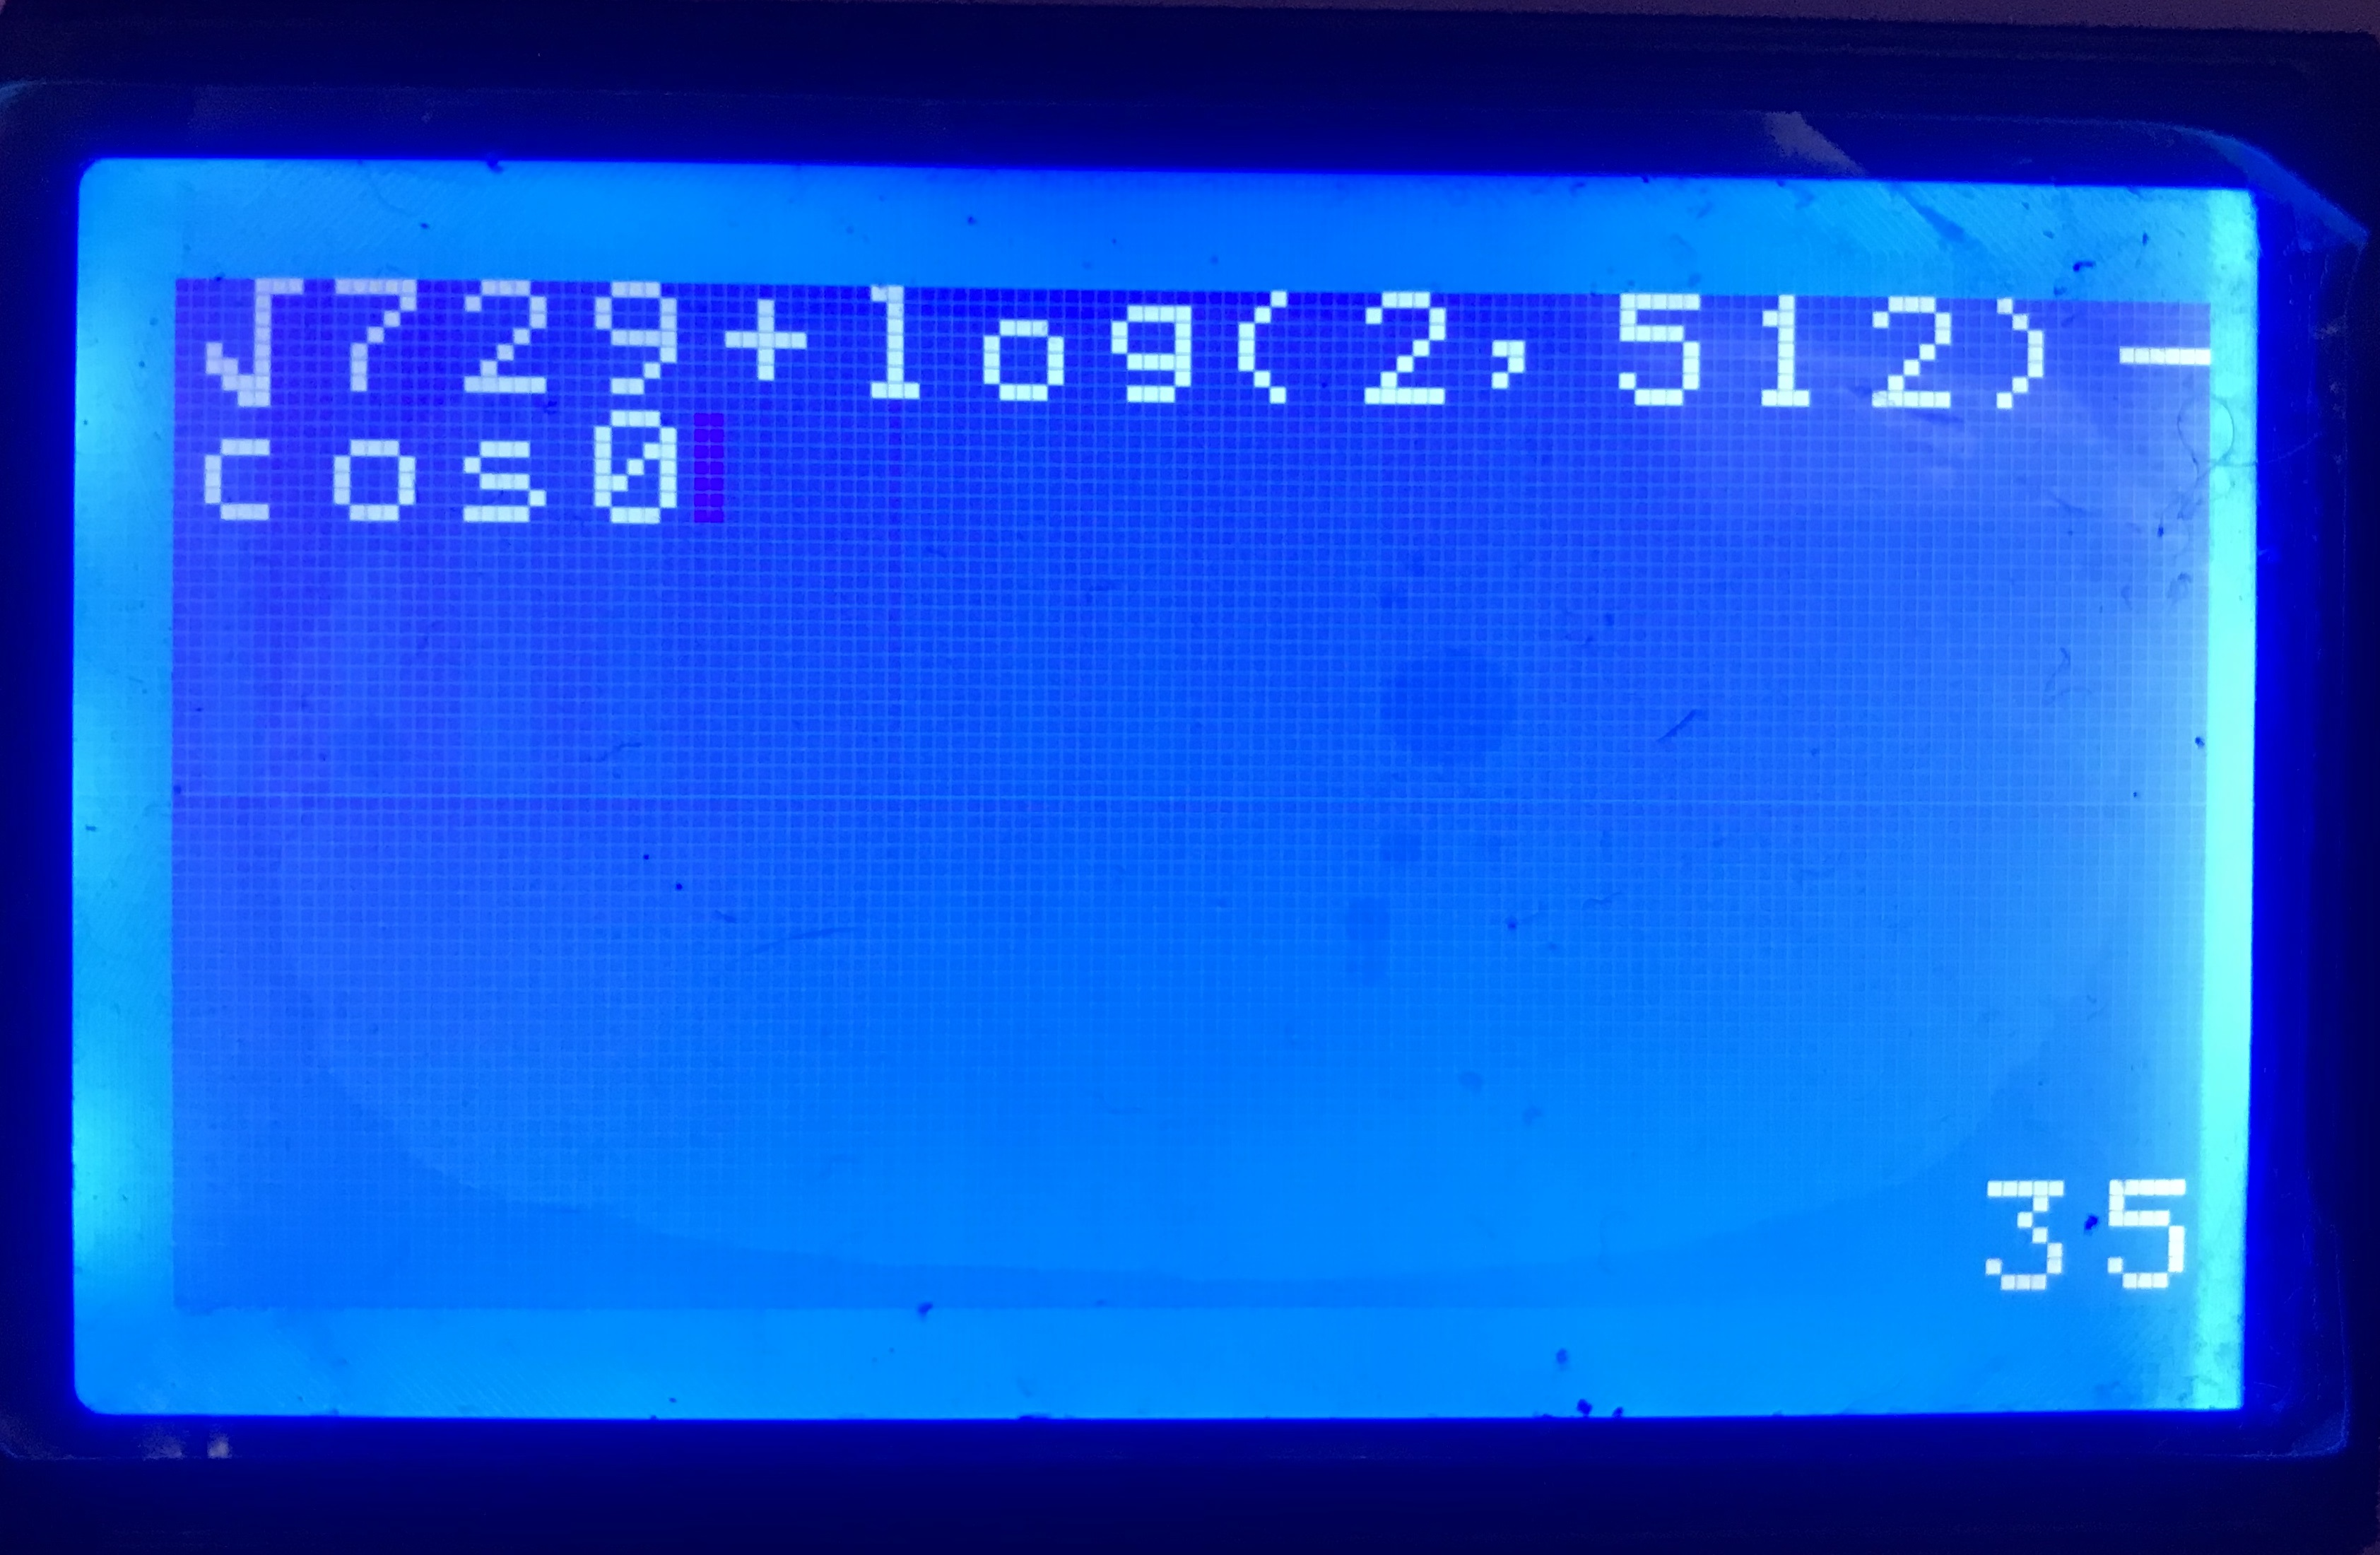
\includegraphics[width=.7\textwidth]{LCDScreens/mathmode.jpeg}
    \caption{Evaluate $\sqrt{729} + \log_2 512 - \cos0$}
\end{figure}

\subsection{Graphing Mode}
The graphing mode of the program enables users to visually explore mathematical functions on a graphical LCD screen. By entering an expression, the program generates a graph that represents the function and displays it in real-time. The graphing mode provides interactive features that allow users to manipulate the graph's properties, such as scaling, centering, and resetting. Users can navigate the graph using intuitive keypad controls, adjusting the position of the graph and zooming in or out to focus on specific areas of interest. Additionally, the graphing mode offers a cursor mode, enabling users to select and examine specific points on the graph, obtaining their coordinates and corresponding function values. This mode provides a dynamic and interactive environment for users to visually analyze and explore mathematical functions with ease.

The \texttt{Graph} function is responsible for drawing a graph on a graphical LCD screen based on a given mathematical expression. It first clears the graphical buffer and calculates the step size based on the scale factor. It determines the display coordinates for the X and Y axes and draws them if they fall within the visible range.

Next, it iterates through the X-axis coordinates from 0 to 127. For each X-coordinate, it evaluates the mathematical expression and calculates the corresponding Y-values, \texttt{y1} and \texttt{y2}. If there is a mathematical error, the Y-value is set to NaN, and the error code is reset. If the error code is greater than 0, indicating a syntax or mathematical error, the function returns.

The Y-coordinates are converted to display coordinates and adjusted to fit within the visible screen range. If at least one of the Y-coordinates is within the visible range, a line is drawn on the screen connecting the two points.

\begin{minted}{c}
void Graph(uint8_t * exp, uint8_t size, uint8_t * errorCode) {
  GLCD_Buf_Clear();
  double step = scale * 2 / 128;

  int dispX0 = centerX / step;
  int dispY0 = -(centerY / step) + 64;

  if (dispX0 >= 0 && dispX0 < 128)
    DrawLine(dispX0, 0, dispX0, 63);

  if (dispY0 >= 0 && dispY0 < 64)
    DrawLine(0, dispY0, 127, dispY0);

  for (int i = 0; i < 127; i++) {
    SetVar(X, i * step - centerX);
    double y1 = evaluate(exp, size, errorCode);
    if ( * errorCode == 4) {
      y1 = NAN;
      * errorCode = 0;
    }

    SetVar(X, (i + 1) * step - centerX);
    double y2 = evaluate(exp, size, errorCode);

    if ( * errorCode == 4) {
      y2 = NAN;
      * errorCode = 0;
    }
    if ( * errorCode > 0)
      return;

    int dispY1 = (y1 + centerY) / step;
    int dispY2 = (y2 + centerY) / step;

    dispY1 = -dispY1 + 64;
    dispY2 = -dispY2 + 64;

    if (!((dispY1 < 0 || dispY1 > 63) && (dispY2 < 0 || dispY2 > 63))) {
      if (dispY1 < 0) dispY1 = 0;
      if (dispY1 > 64) dispY1 = 63;
      if (dispY2 < 0) dispY2 = 0;
      if (dispY2 > 64) dispY2 = 63;
      DrawLine(i, dispY1, i + 1, dispY2);
    }
  }
}
\end{minted}

The \texttt{GraphScreen} function is responsible for displaying the graph on the screen and handling user interactions. It calls the \texttt{Graph} function to initially draw the graph.

It then enters a loop to listen for key inputs. If the user is not in cursor mode, the function handles various key inputs to adjust the graph's properties, such as centering, scaling, and resetting. If the user enters the cursor mode (by pressing the \texttt{TEST} key), the current graph is stored, and the cursor mode is activated.

If the user is in cursor mode, the function handles left and right key inputs to move the cursor horizontally on the graph. If the cursor is within the valid range, a horizontal and vertical dashed line is drawn to indicate its position, and the exact coordinate is shown in the answer row. If the user enters any other key, the cursor mode is exited, the original graph is restored, and the loop continues.

\begin{minted}{c}
void GraphScreen(uint8_t * exp, uint8_t size, uint8_t * errorCode) {
  double t = GetVar(X);
  Graph(exp, input_length, errorCode);

  if ( * errorCode > 0) {
    SetVar(X, t);
    return;
  }

  ST7920_Update();
  while (1) {
    uint8_t key = KeyPad_WaitForKeyGetChar(KEY_TIMEOUT_MS, true);
    if (key != 0xFF) {
      double step = (scale * 2 / 128);
      double moveStep = step * 5;

      if (!cursorMode) {
        switch (key) {
        case LEFT:
          centerX += moveStep;
          break;

        case RIGHT:
          centerX -= moveStep;
          break;

        case DOWN:
          centerY += moveStep;
          break;

        case UP:
          centerY -= moveStep;
          break;

        case PLUS:
          scale -= 0.5;
          break;

        case MINUS:
          scale += 0.5;
          break;

        case ZERO:
          scale = 1; centerX = 1; centerY = 0.5;
          break;

        case TEST:
          memcpy(orig_graph, GLCD_Buf, 1024);
          cursorX = 64;
          cursorMode = true;
          break;

        default:
          SetVar(X, t);
          return;
        }
      } else {
        switch (key) {
        case LEFT:
          if (cursorX > 0) cursorX -= 1;
          break;

        case RIGHT:
          if (cursorX < 127) cursorX += 1;
          break;

        default:
          cursorMode = false;
          memcpy(GLCD_Buf, orig_graph, 1024);
          ST7920_Update();
          continue;
        }
      }

      if (cursorMode) {
        memcpy(GLCD_Buf, orig_graph, 1024);
        double x = cursorX * step - centerX;
        SetVar(X, x);
        double y = evaluate(exp, size, errorCode);
        if ( * errorCode == 4) {
          y = NAN;
          * errorCode = 0;
        }

        uint8_t cursorY = (y + centerY) / step;
        cursorY = -cursorY + 64;

        DrawDashedLine(cursorX, 0, cursorX, 63, 2, 3);
        if (cursorY < 64 && cursorY >= 0)
          DrawDashedLine(0, cursorY, 127, cursorY, 2, 3);

        sprintf((char * ) answerRow_buf, "%0.3g;%0.3g", x, y);
        PrintAnswer();
      } else
        Graph(exp, input_length, errorCode);
      ST7920_Update();
    }
  }
}
\end{minted}

\begin{figure}[H]
    \centering
    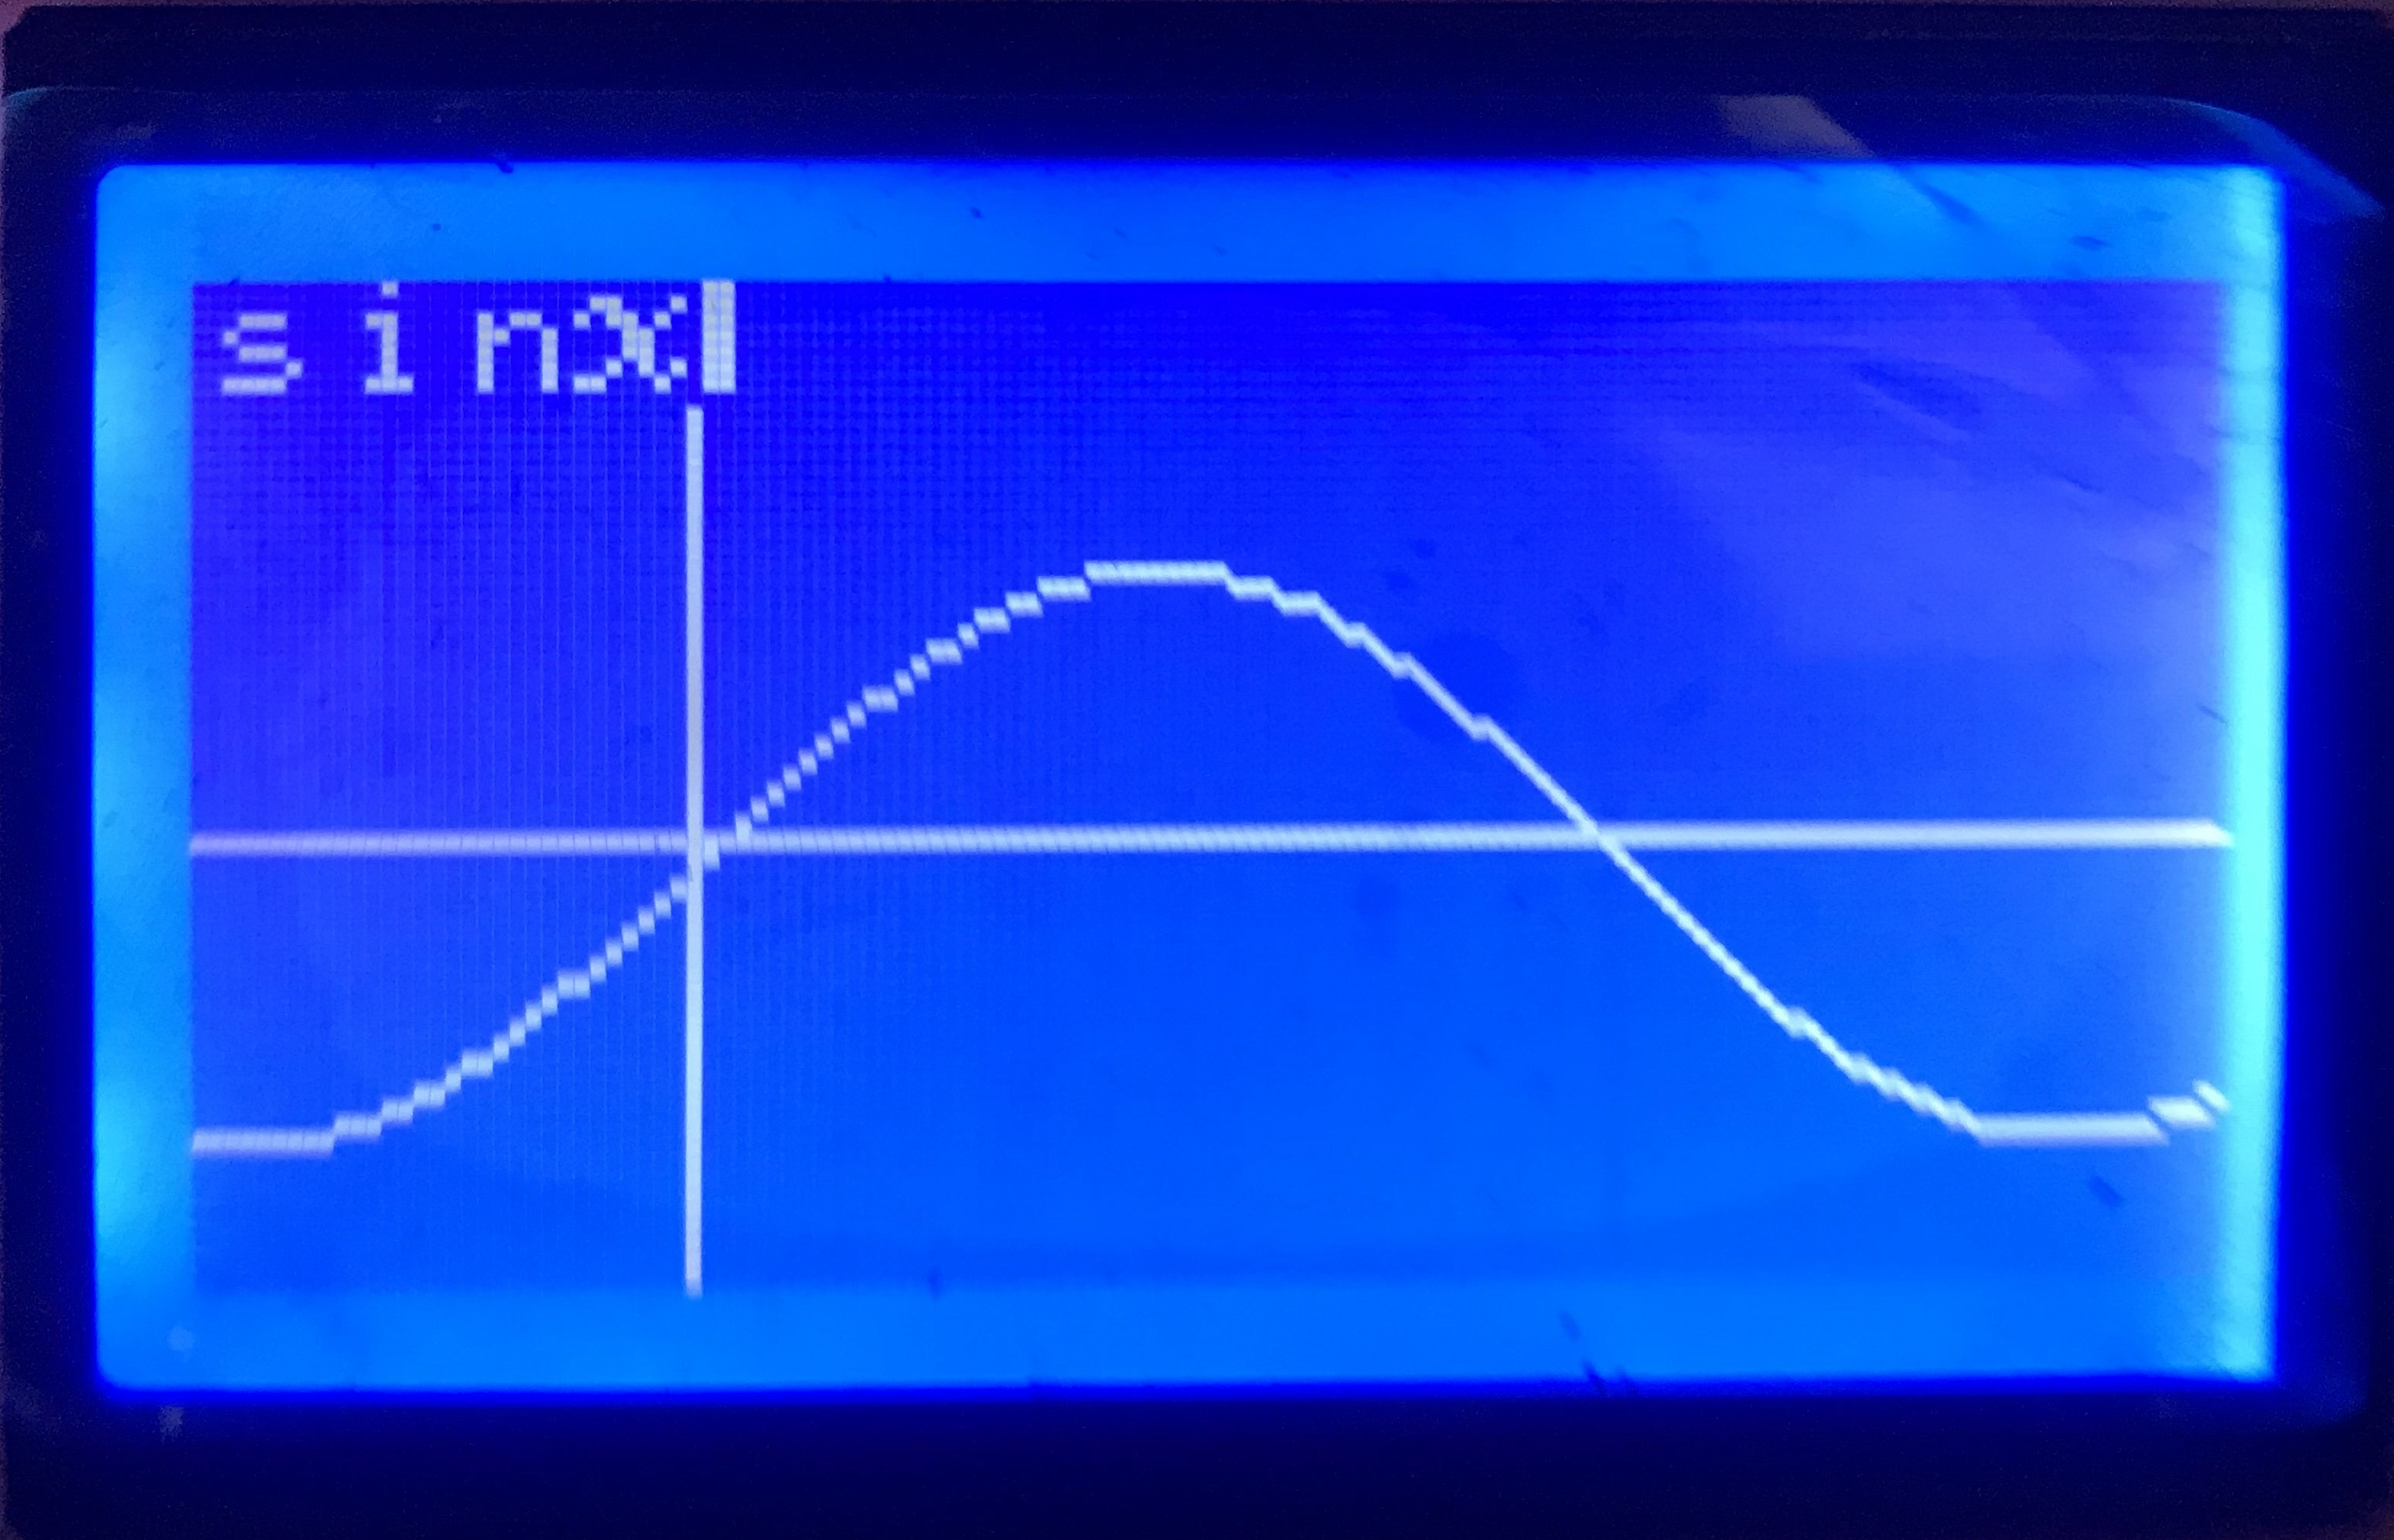
\includegraphics[width=.7\textwidth]{LCDScreens/graphmode.jpeg}
    \caption{Graphing $\sin x$}
\end{figure}

\section{UART Communication with Computer}

One innovative idea to improve the calculation speed on the microcontroller unit (MCU) and leverage the computing power of a computer is by establishing a UART (Universal Asynchronous Receiver-Transmitter) connection between the MCU and a PC. By connecting the MCU to the computer using a TTL to USB converter, we can send complex mathematical expressions from the calculator to the PC for evaluation. The PC, equipped with more computational resources, can efficiently perform the calculations and send back the results to the calculator. This approach allows us to offload the heavy computation to the PC, enabling faster and more complex calculations on our calculator device. Furthermore, with the potential implementation of a UART Bluetooth or Wi-Fi module in the future, you can expand the connectivity options and make the calculator wirelessly communicate with other devices for enhanced functionality.

\begin{figure}[H]
    \centering
    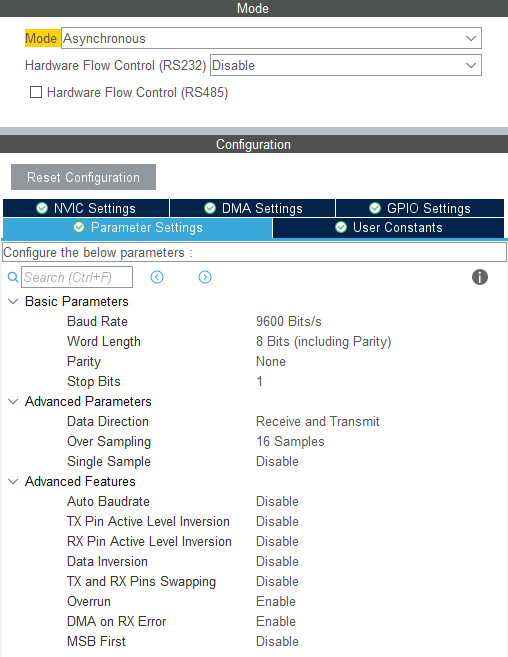
\includegraphics[scale=0.7]{Software/UART_settings.png}
    \caption{UART settings}
\end{figure}

\mintinline{c}{HAL_UART_Transmit(&huart2, pData, size, HAL_MAX_DELAY)} is used to transmit data over UART using the HAL library. When in UART mode (toggle by \texttt{TEST} button, indicated by top-right pixel of the LCD), and press the \texttt{EQUAL} button, the input buffer will sent to computer, and the program will wait for the response with 3s timeout.

There are three modes for USART receive: polling, interrupt and DMA (Direct Memory Access). In comparison to polling and DMA modes, interrupt mode offers a balance between simplicity and efficiency for UART communication in STM32 microcontrollers. Polling mode is straightforward but can consume more CPU resources due to constant checking. DMA mode is efficient for large data transfers but adds complexity in configuration and management. Interrupt mode provides a good compromise, allowing the CPU to be notified only when data is available for transmission or reception, reducing CPU overhead and improving system performance. It strikes a balance by providing efficient CPU utilization without the added complexity of DMA. Therefore, interrupt mode is often a favorable choice for UART communication in STM32 applications.

% \begin{figure}[H]
%     \centering
%     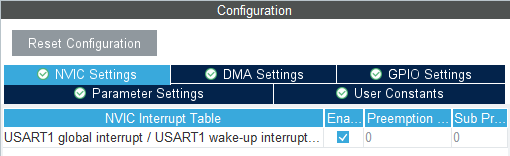
\includegraphics[scale=0.9]{Software/UART_interrupt.png}
%     \caption{USART global interrupt settings}
% \end{figure}

To use interrupt, we need to set USART global interrupt in NVIC settings. To enable USART interrupt, \texttt{HAL\_UART\_Receive\_IT()} can be used. This function prepares the USART peripheral to trigger an interrupt whenever data is received. The function \mintinline{c}{HAL_UART_Receive_IT(&huart1, (uint8_t*) RxBuf, 8)} initiates the reception of 8 bytes of data (size of double) into the buffer \texttt{RxBuf} using the UART peripheral huart1.

And here interrupt handler function for the USART receive interrupt. This function will be called by the microcontroller whenever the data is fully received.

\begin{minted}{c}
void HAL_UART_RxCpltCallback(UART_HandleTypeDef *huart) {
  if (huart->Instance == USART1) {
    uartDone = true;
    /* start the INT again */
    HAL_UART_Receive_IT (&huart1, RxBuf, RxBuf_SIZE);
  }
}
\end{minted}

The \texttt{uartDone} then break the while loop of the wait function, and show the result onto the answer row. If timeout of 3 seconds exceed, with \texttt{uartDone == false}, \texttt{Receive Failed} will show onto the answer row.

\begin{minted}{c}
//...
            if (uartMode) {
              uartDone = false;
              HAL_UART_Transmit( & huart1, input, input_length, 100);

              millis = HAL_GetTick();

              while (HAL_GetTick() - millis <= 3000) {
                if (uartDone) break;
              }

              if (!uartDone) {
                strcpy(answerRow_buf, "Receive Failed.");
                PrintAnswer();
              } else {
                memcpy( & answer, RxBuf, sizeof(double));
                errorCode = RxBuf[8];

                if (errorCode == 0) SetVar(ANSWER, answer);
                ShowAnswer(answer, errorCode);
              }
            }
//...
\end{minted}

We are done with the device side, now we need to write a program on Windows to receive and transmit data to the calculator. Below is a simple program running on a Windows platform that establishes communication over a serial port (COM4) and receives data from an external device connected to that port.

\begin{minted}{c}
#include <Windows.h>
#include <stdio.h>

#include "KeyPad/KeyPad.h"
#include "EvalExpr/EvalExpr.h"
#include "EvalExpr/EvalExpr.c"

char input[256];
uint8_t input_length = 0;

void main(void) {
  InitSto();

  DWORD dwCommEvent;
  DWORD dwRead;
  DWORD dwWritten;
  DWORD lpEvtMask;
  char chRead;
  char ComPortName[] = "\\\\.\\COM4";
  int i = 0;

  HANDLE hComm;
  hComm = CreateFile(ComPortName,
    GENERIC_READ | GENERIC_WRITE,
    0,
    0,
    OPEN_EXISTING,
    0,
    0);
  if (hComm == INVALID_HANDLE_VALUE)
    printf("Error opening port.\n");

  //////////////////////////////////////////////////////
  DCB dcb;

  FillMemory( & dcb, sizeof(dcb), 0);
  if (!GetCommState(hComm, & dcb)) // get current DCB
    printf("Error GetCommState.\n");

  // Update DCB rate.
  dcb.BaudRate = CBR_9600;
  dcb.ByteSize = 8; // Setting ByteSize = 8
  dcb.StopBits = ONESTOPBIT; // Setting StopBits = 1
  dcb.Parity = NOPARITY; // Setting Parity = None
  dcb.DCBlength = sizeof(dcb);
  // Set new state.
  if (!SetCommState(hComm, & dcb))
    printf("Error SetCommState.\n");
  // Error in SetCommState. Possibly a problem with the communications
  // port handle or a problem with the DCB structure itself.

  /////////////////////////////////////////////////////////////////////
  COMMTIMEOUTS timeouts;

  timeouts.ReadIntervalTimeout = MAXDWORD;
  timeouts.ReadTotalTimeoutMultiplier = 100;
  timeouts.ReadTotalTimeoutConstant = 100;
  timeouts.WriteTotalTimeoutMultiplier = 100;
  timeouts.WriteTotalTimeoutConstant = 100;

  if (!SetCommTimeouts(hComm, & timeouts))
    printf("Error timeouts.\n");

  if (!PurgeComm(hComm, PURGE_RXCLEAR | PURGE_TXCLEAR | PURGE_RXABORT | PURGE_TXABORT))
    printf("Error PurgeComm.\n");
  ////////////////////////////////////////
  for (;;) {
    if (!SetCommMask(hComm, 0))
      printf("Error CommMask.\n");

    if (!SetCommMask(hComm, EV_RXCHAR))
      printf("Error CommMask.\n");

    printf("Waiting for characters.. \n\n");

    if (WaitCommEvent(hComm, & dwCommEvent, NULL)) {
      input_length = 0;
      do {
        if (ReadFile(hComm, & chRead, 1, & dwRead, NULL)) {
          if (dwRead != 0) {
            // printf("Character Received: %d\n",chRead & 0xFF);
            input[input_length] = chRead;
            input_length++;
          }
        } else {
          printf("ErrorReadFile.\n");
          break;
        }
      } while (dwRead);

      if (input_length > 0) {
        printf("Received: ");
        for (int i = 0; i < input_length; i++) {
          printf("%d ", input[i] & 0xFF);
        }
        printf("\n");
        uint8_t errorCode = 0;
        double result = evaluate(input, input_length, & errorCode);
        printf("%f, %d\n", result, errorCode);

        WriteFile(hComm, & result, sizeof(double), & dwWritten, NULL);
        WriteFile(hComm, & errorCode, 1, & dwWritten, NULL);
      }
    } else {
      printf("Error WaitCommEvent.\n");
      break;
    }
    printf("=========================\n");
  }
}
\end{minted}


\chapter{Result}
\section{The device}
\begin{figure}[H]
    \centering
    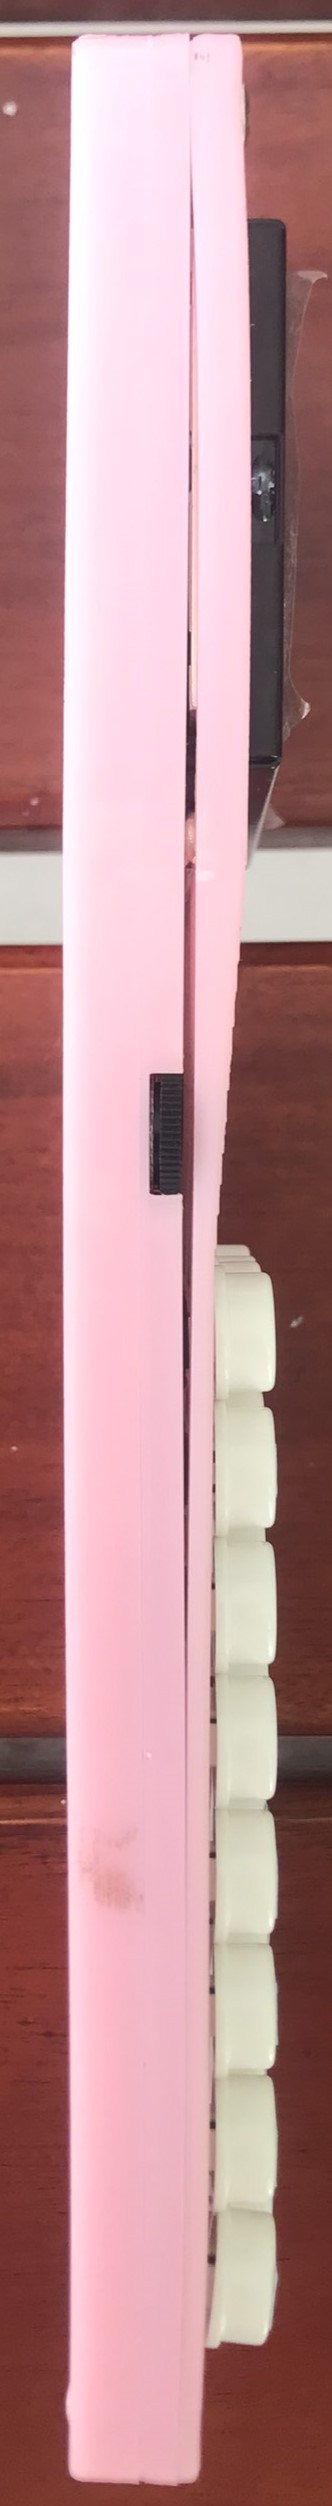
\includegraphics[height=.7\textheight]{3DCase/leftside_view.jpg}\qquad
    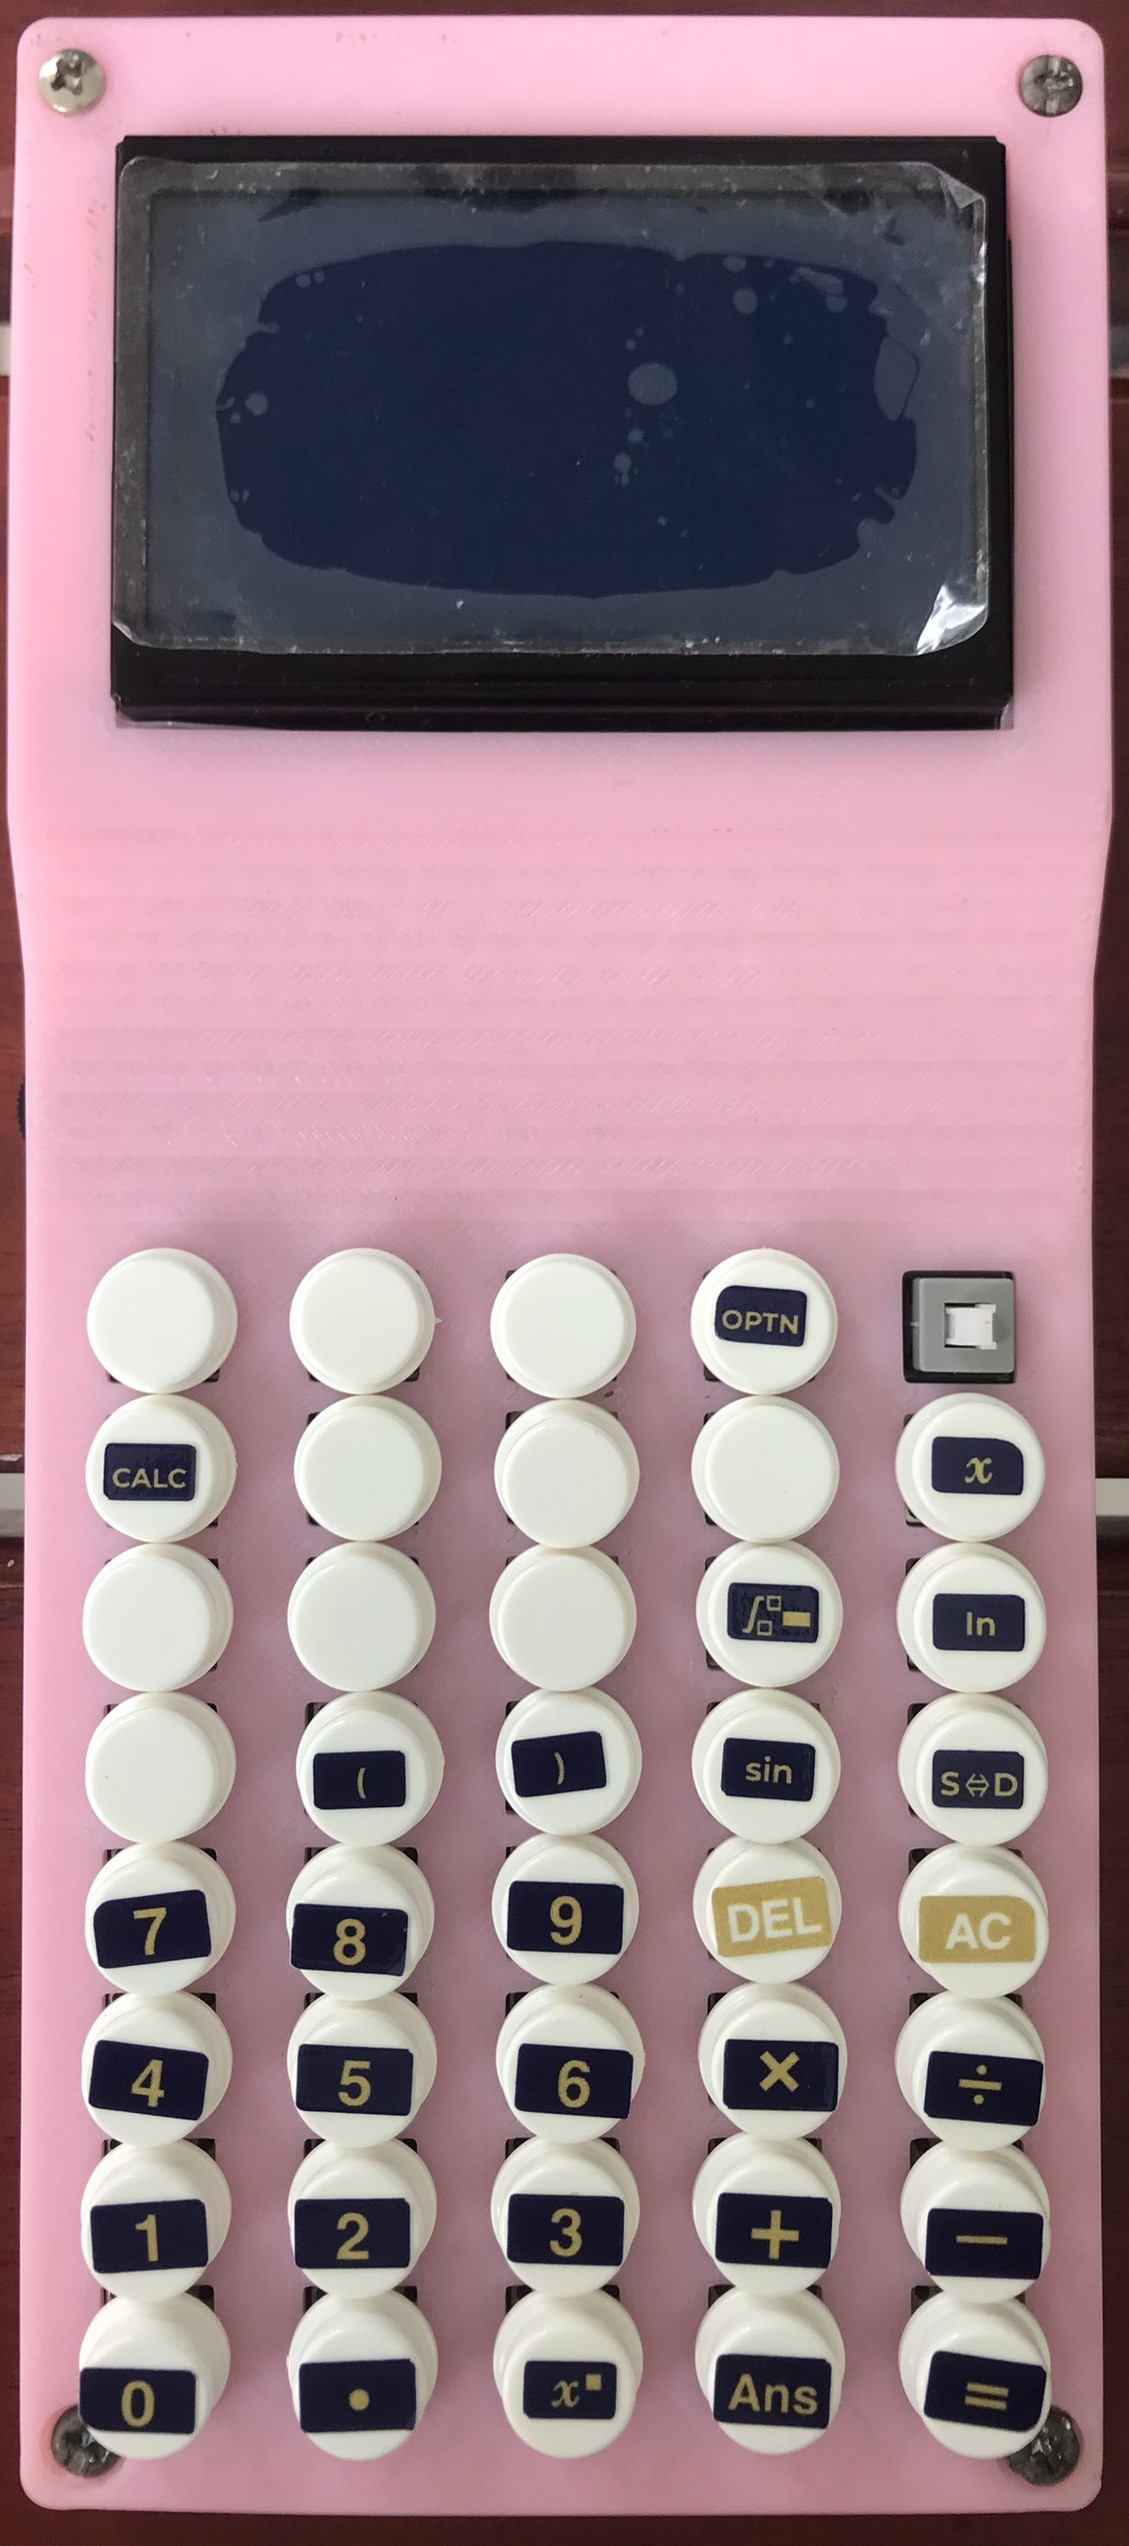
\includegraphics[height=.7\textheight]{3DCase/frontview.jpg}\qquad
    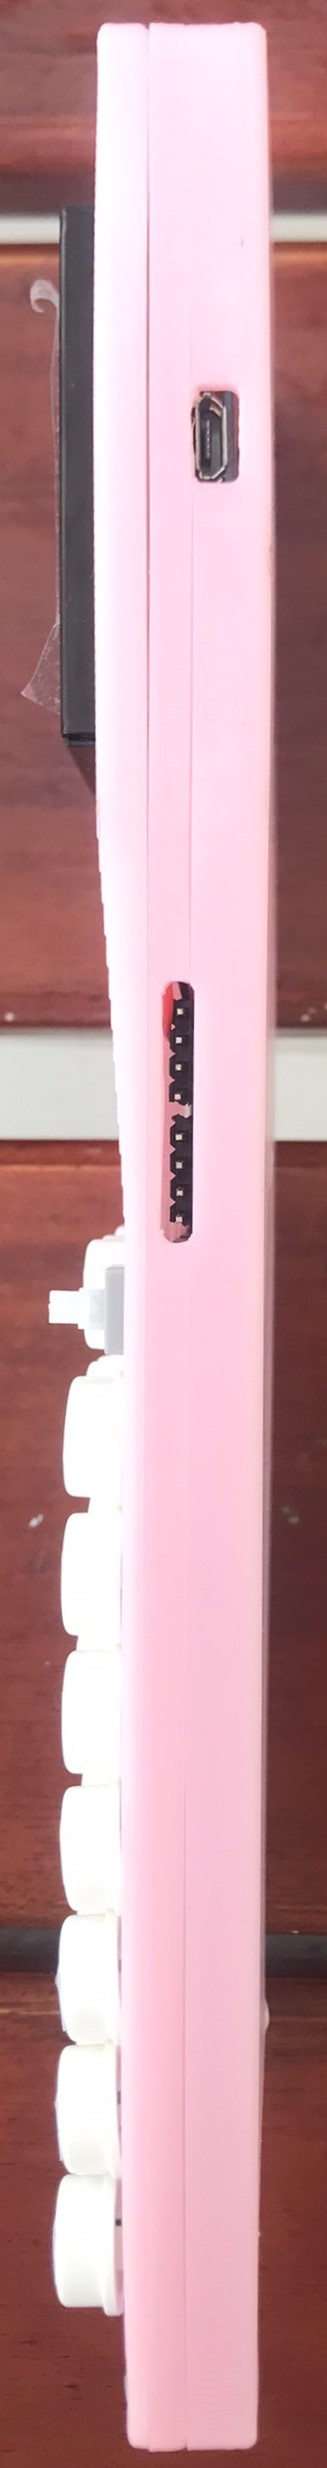
\includegraphics[height=.7\textheight]{3DCase/rightside_view.jpg}
    \caption{Front and side view of the device}
\end{figure}

\newpage
\section{Power Consumption}
\begin{table}[H]
    \centering
    \begin{tabular}{|l|l|}
    \hline
        \textbf{Brightness} & \textbf{Power Consumption (W)} \\ \hline
        0\% & 24mA \\ \hline
        50\% & 46mA \\ \hline
        100\% & 68mA \\ \hline
    \end{tabular}
    \caption{Power consumption at 0\%, 50\% and 100\% brightness level}
\end{table}

For real world estimation, assume that users would use the calculator at 70\% brightness, we can calculate the average power consumption per hour based on the provided data from the table.

At 70\% brightness, the power consumption is 46mA. Since the battery capacity is 1200mAh, we can calculate the estimated battery life = 1200mAh / 46mA $\approx$ 26.09 hours.

Therefore, when using the calculator at 70\% brightness, the estimated battery life would be approximately 26.09 hours. Assume users use the calculator one hour of total time per day, the estimated battery life would be approximately 26.09 days. Keep in mind that this is an estimation, and the actual battery life may vary depending on factors such as the efficiency of the battery, other components of the calculator and also the environment.

\section{Software demonstration}
\begin{figure}[H]
    \centering
    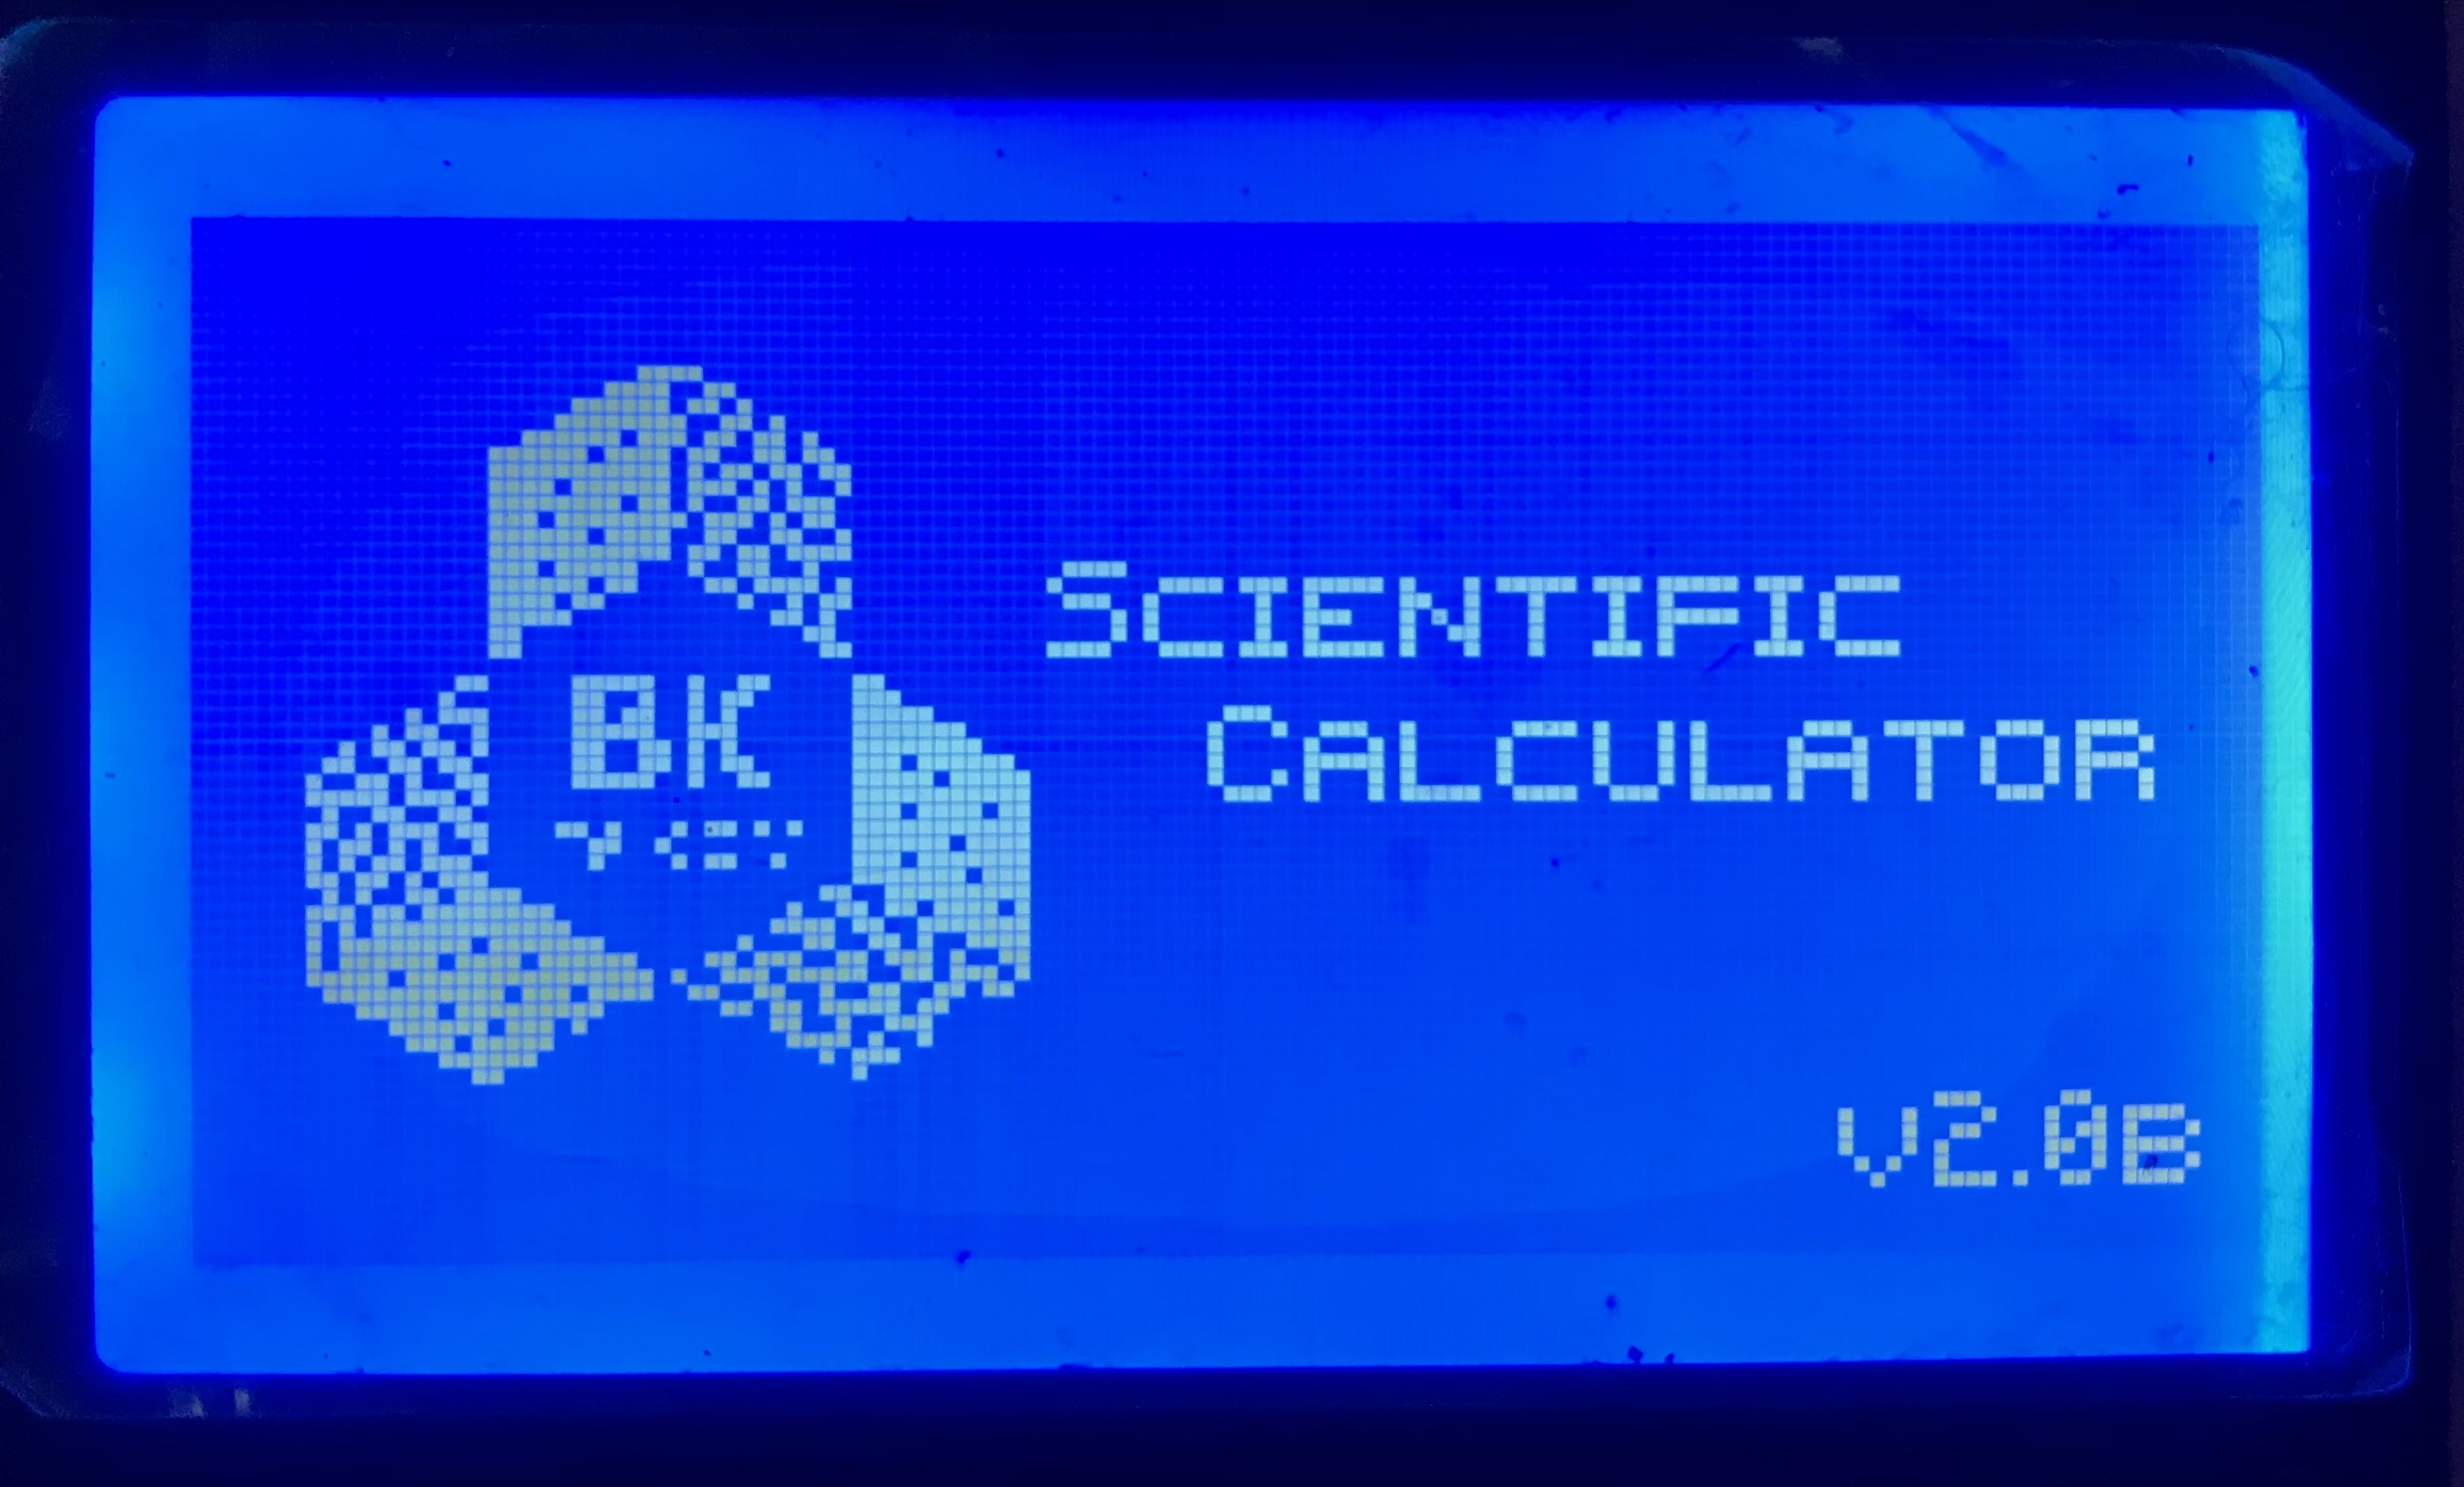
\includegraphics[width=.7\textwidth]{LCDScreens/splash.jpeg}
    \caption{Splash Screen on bootup}
\end{figure}

\newpage
\begin{figure}[H]
    \centering
    \subfloat[][Evaluate $2\times 5 + 2^5 + 13\times 2$]{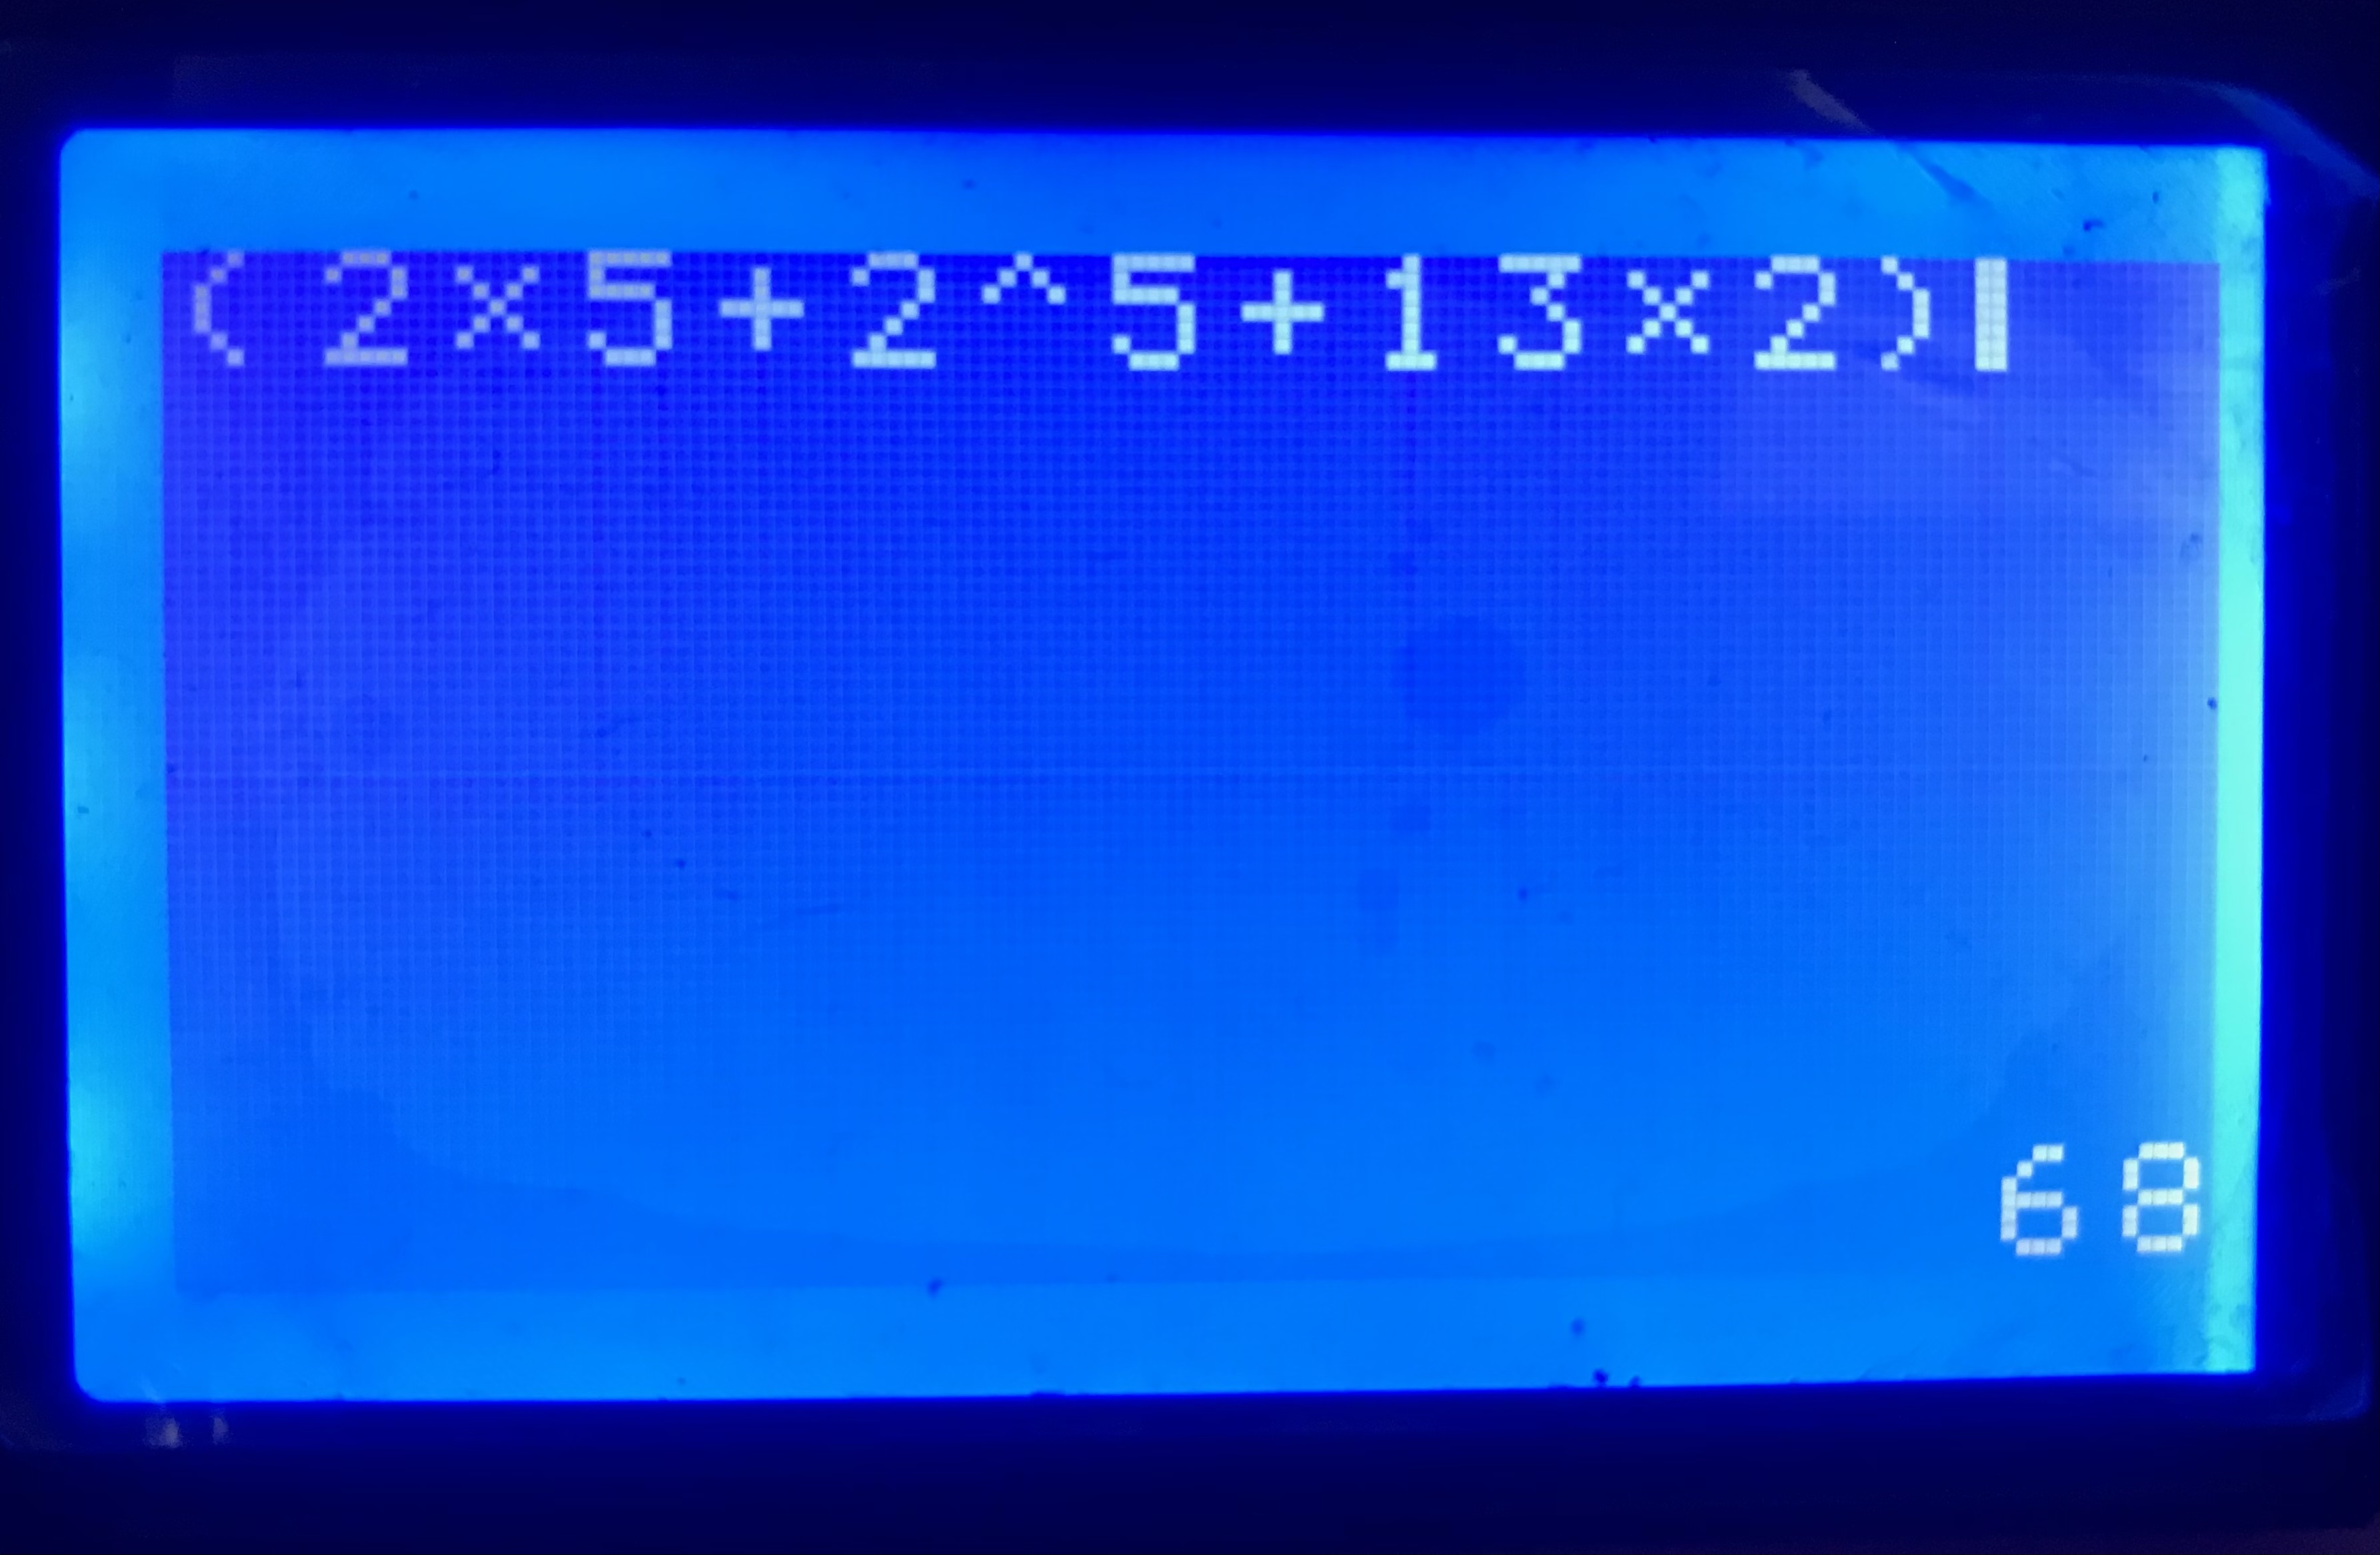
\includegraphics[width=.45\textwidth]{LCDScreens/basicmath.jpeg}}\quad
    \subfloat[][Evaluate $\sin\frac{\pi}{2}$]{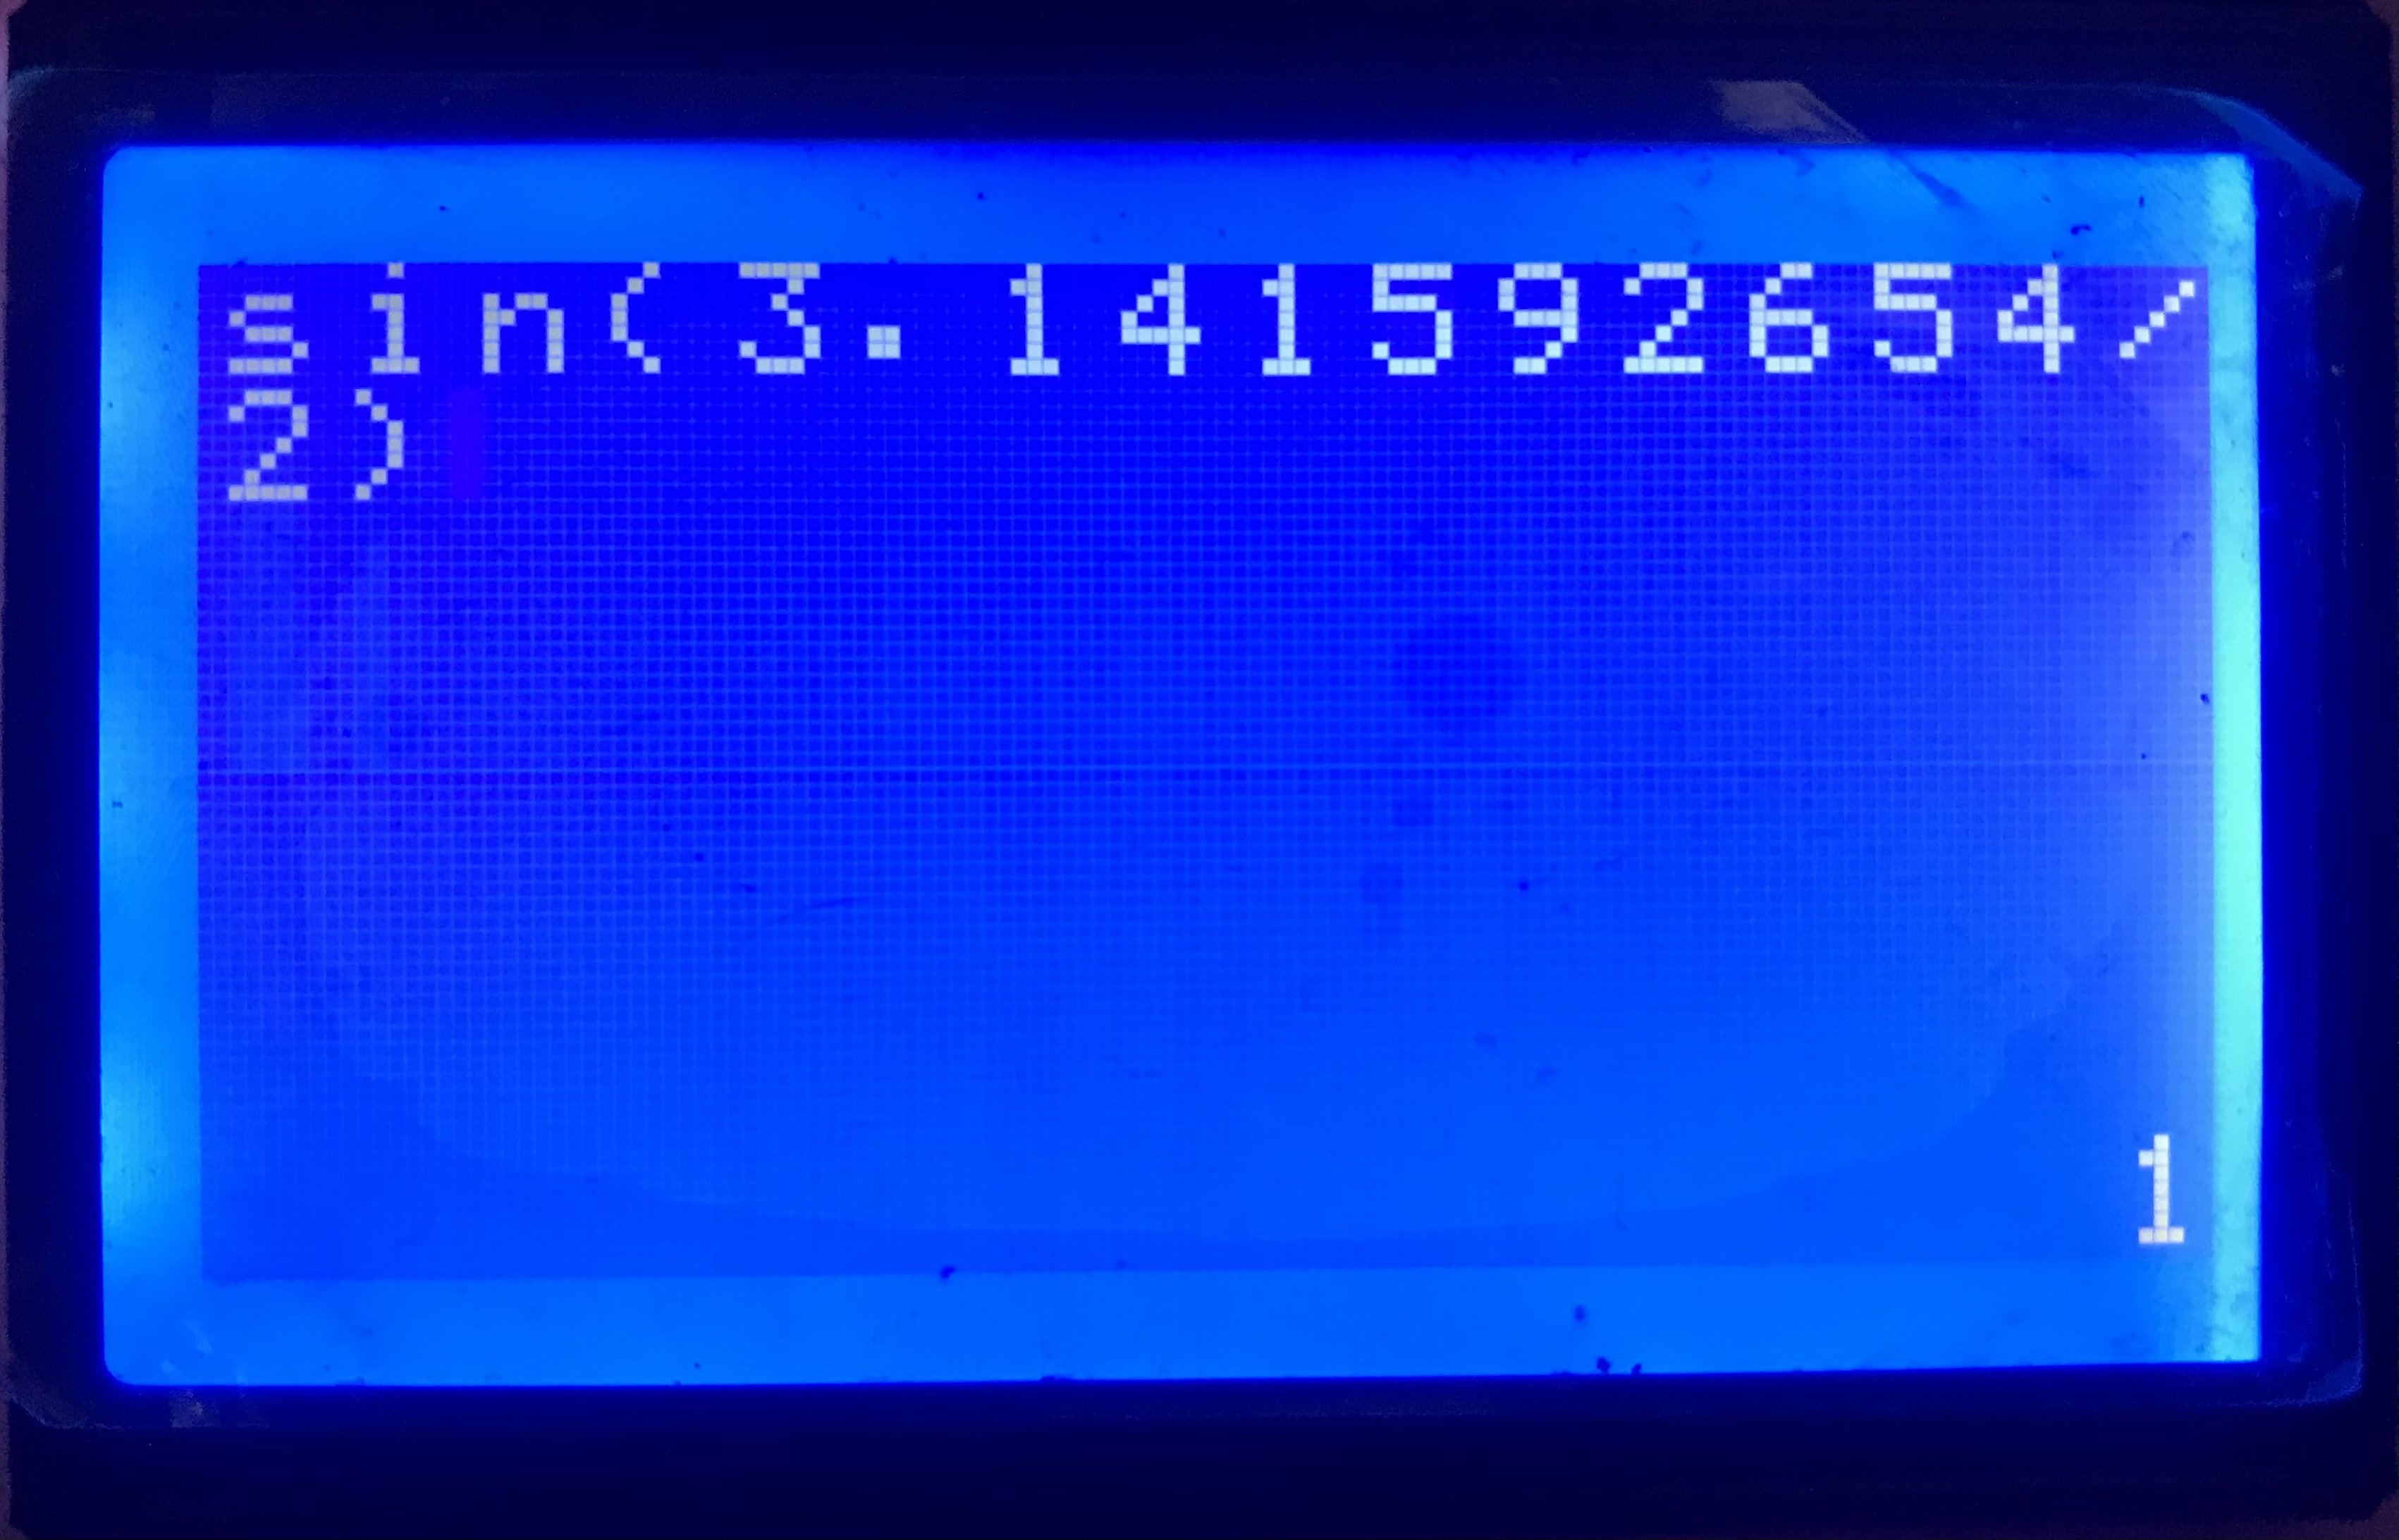
\includegraphics[width=.45\textwidth]{LCDScreens/trig.jpeg}}
    
    \subfloat[][Evaluate $\lim_{x\to +\inf}\frac{1}{x}$]{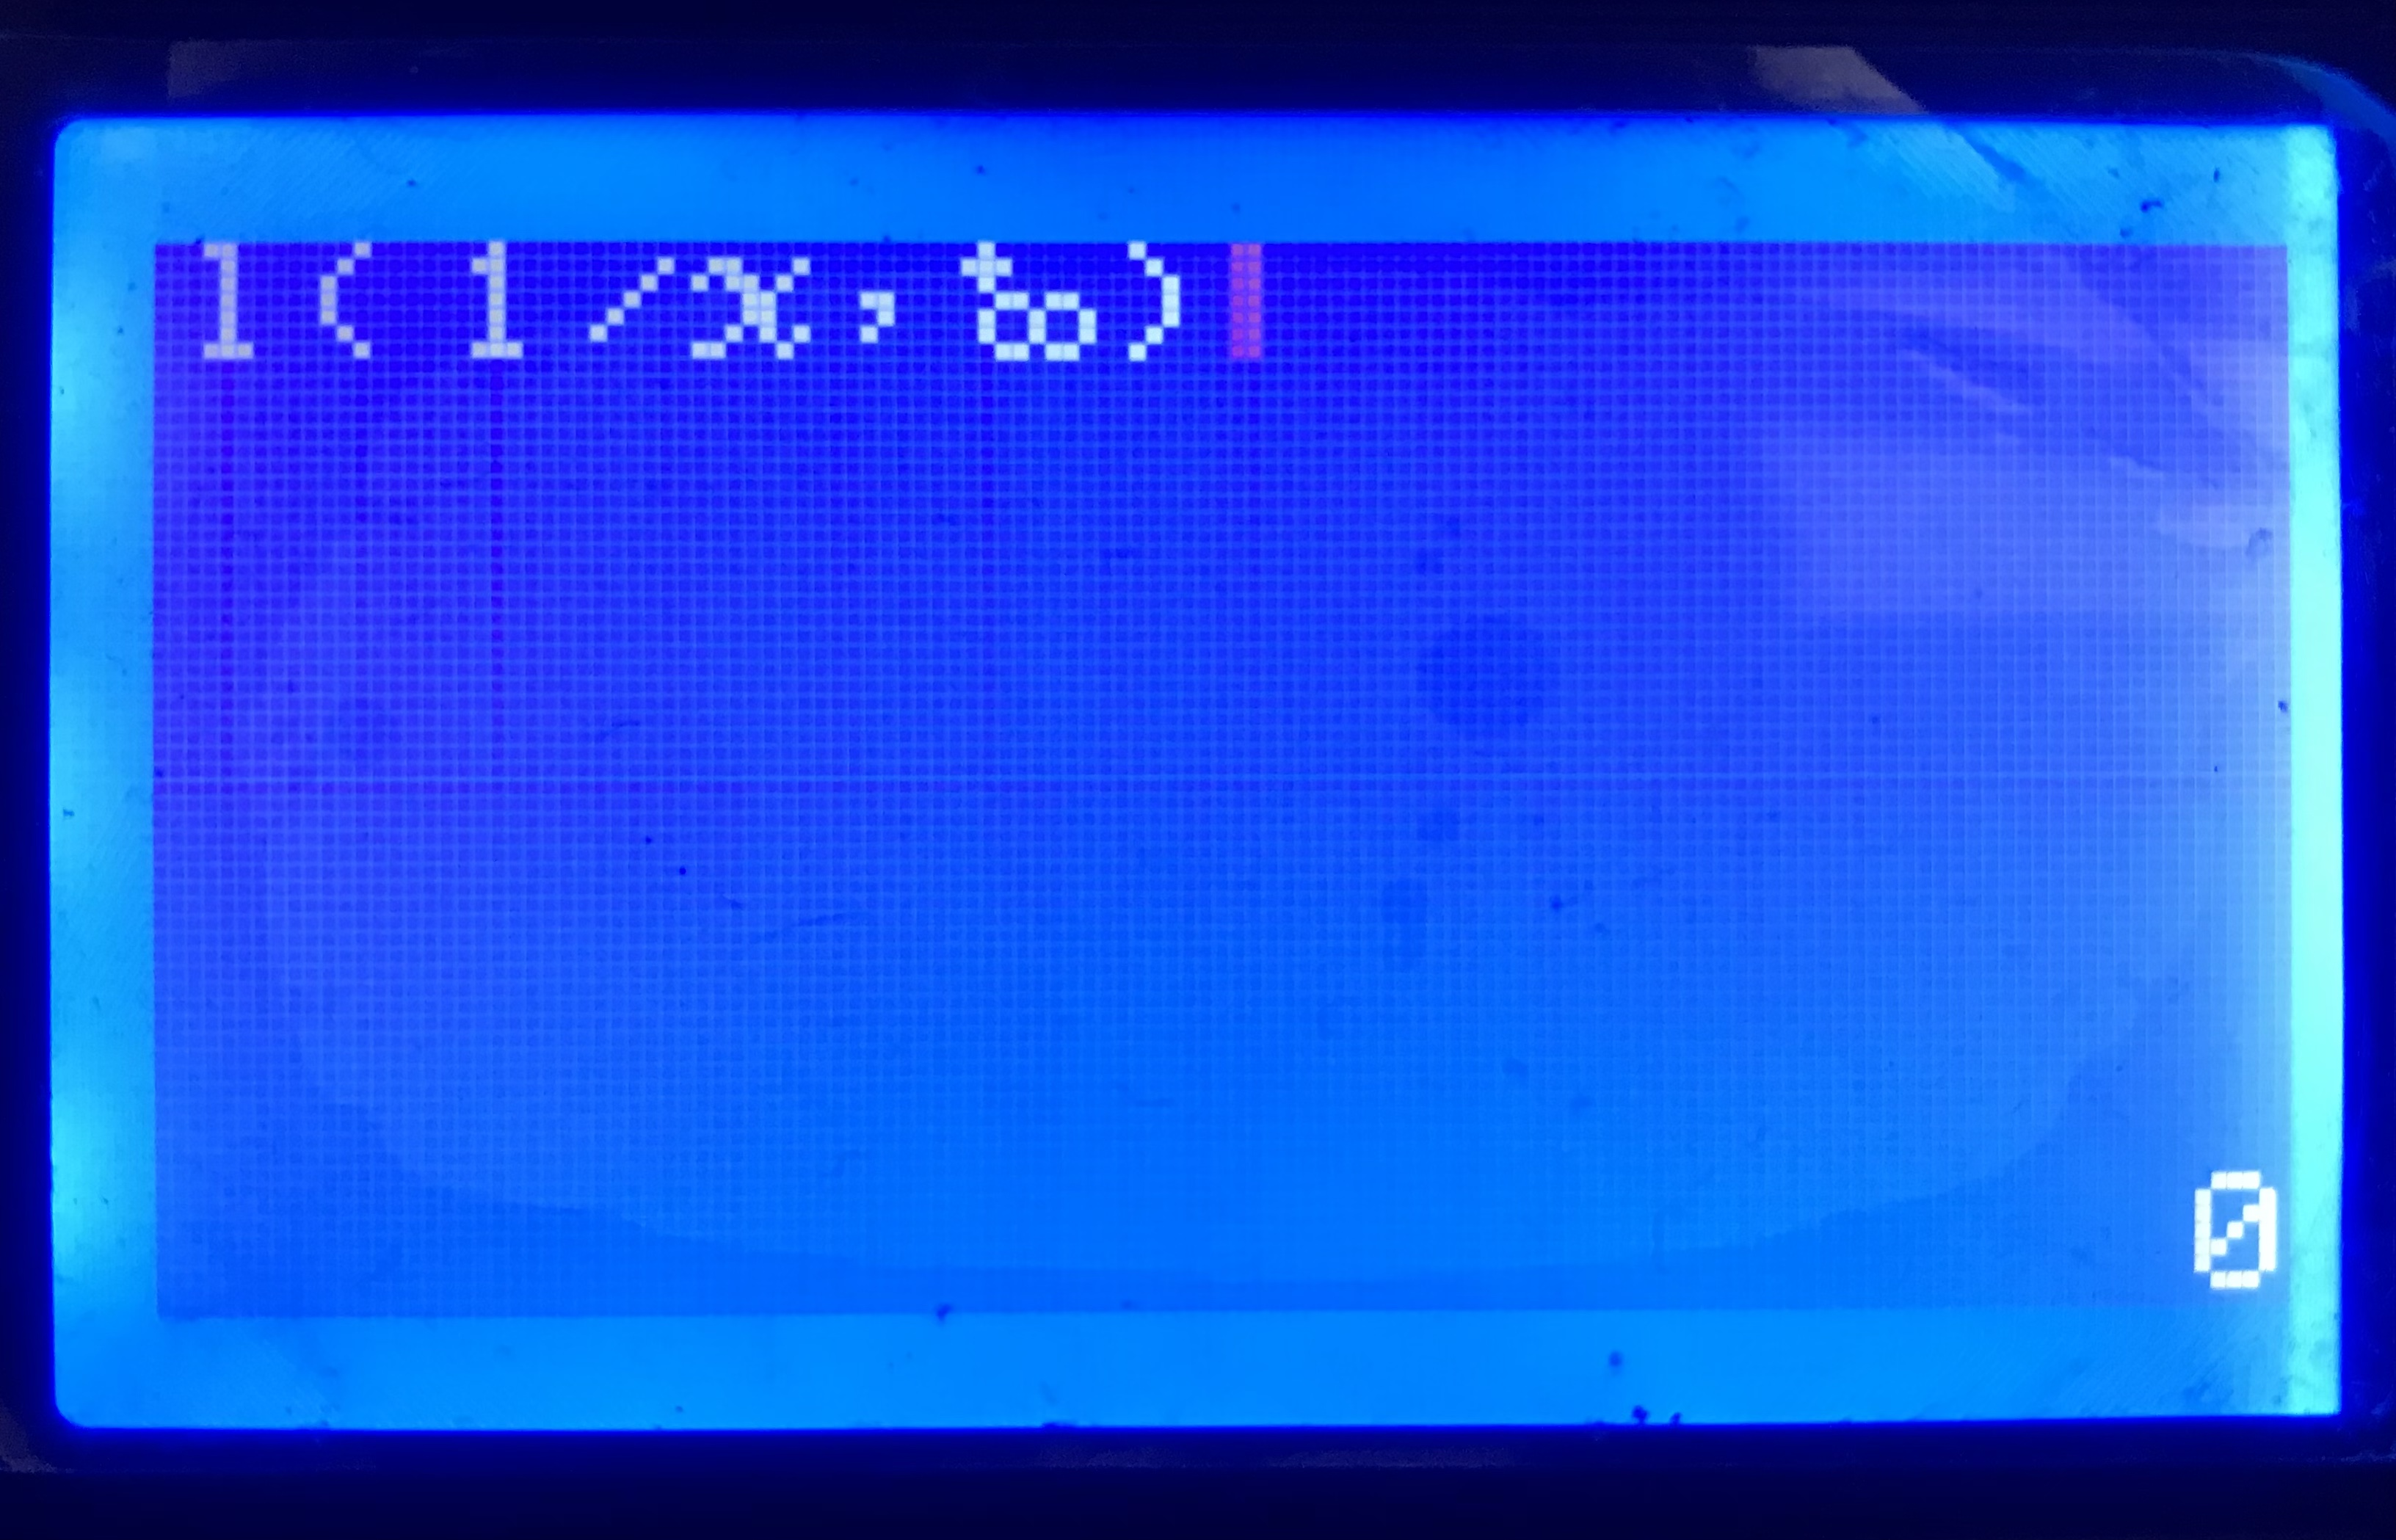
\includegraphics[width=.45\textwidth]{LCDScreens/lim.jpeg}}\quad
    \subfloat[][Evaluate $\frac{d}{dx}x^x$ at $x=3$ (basic math)]{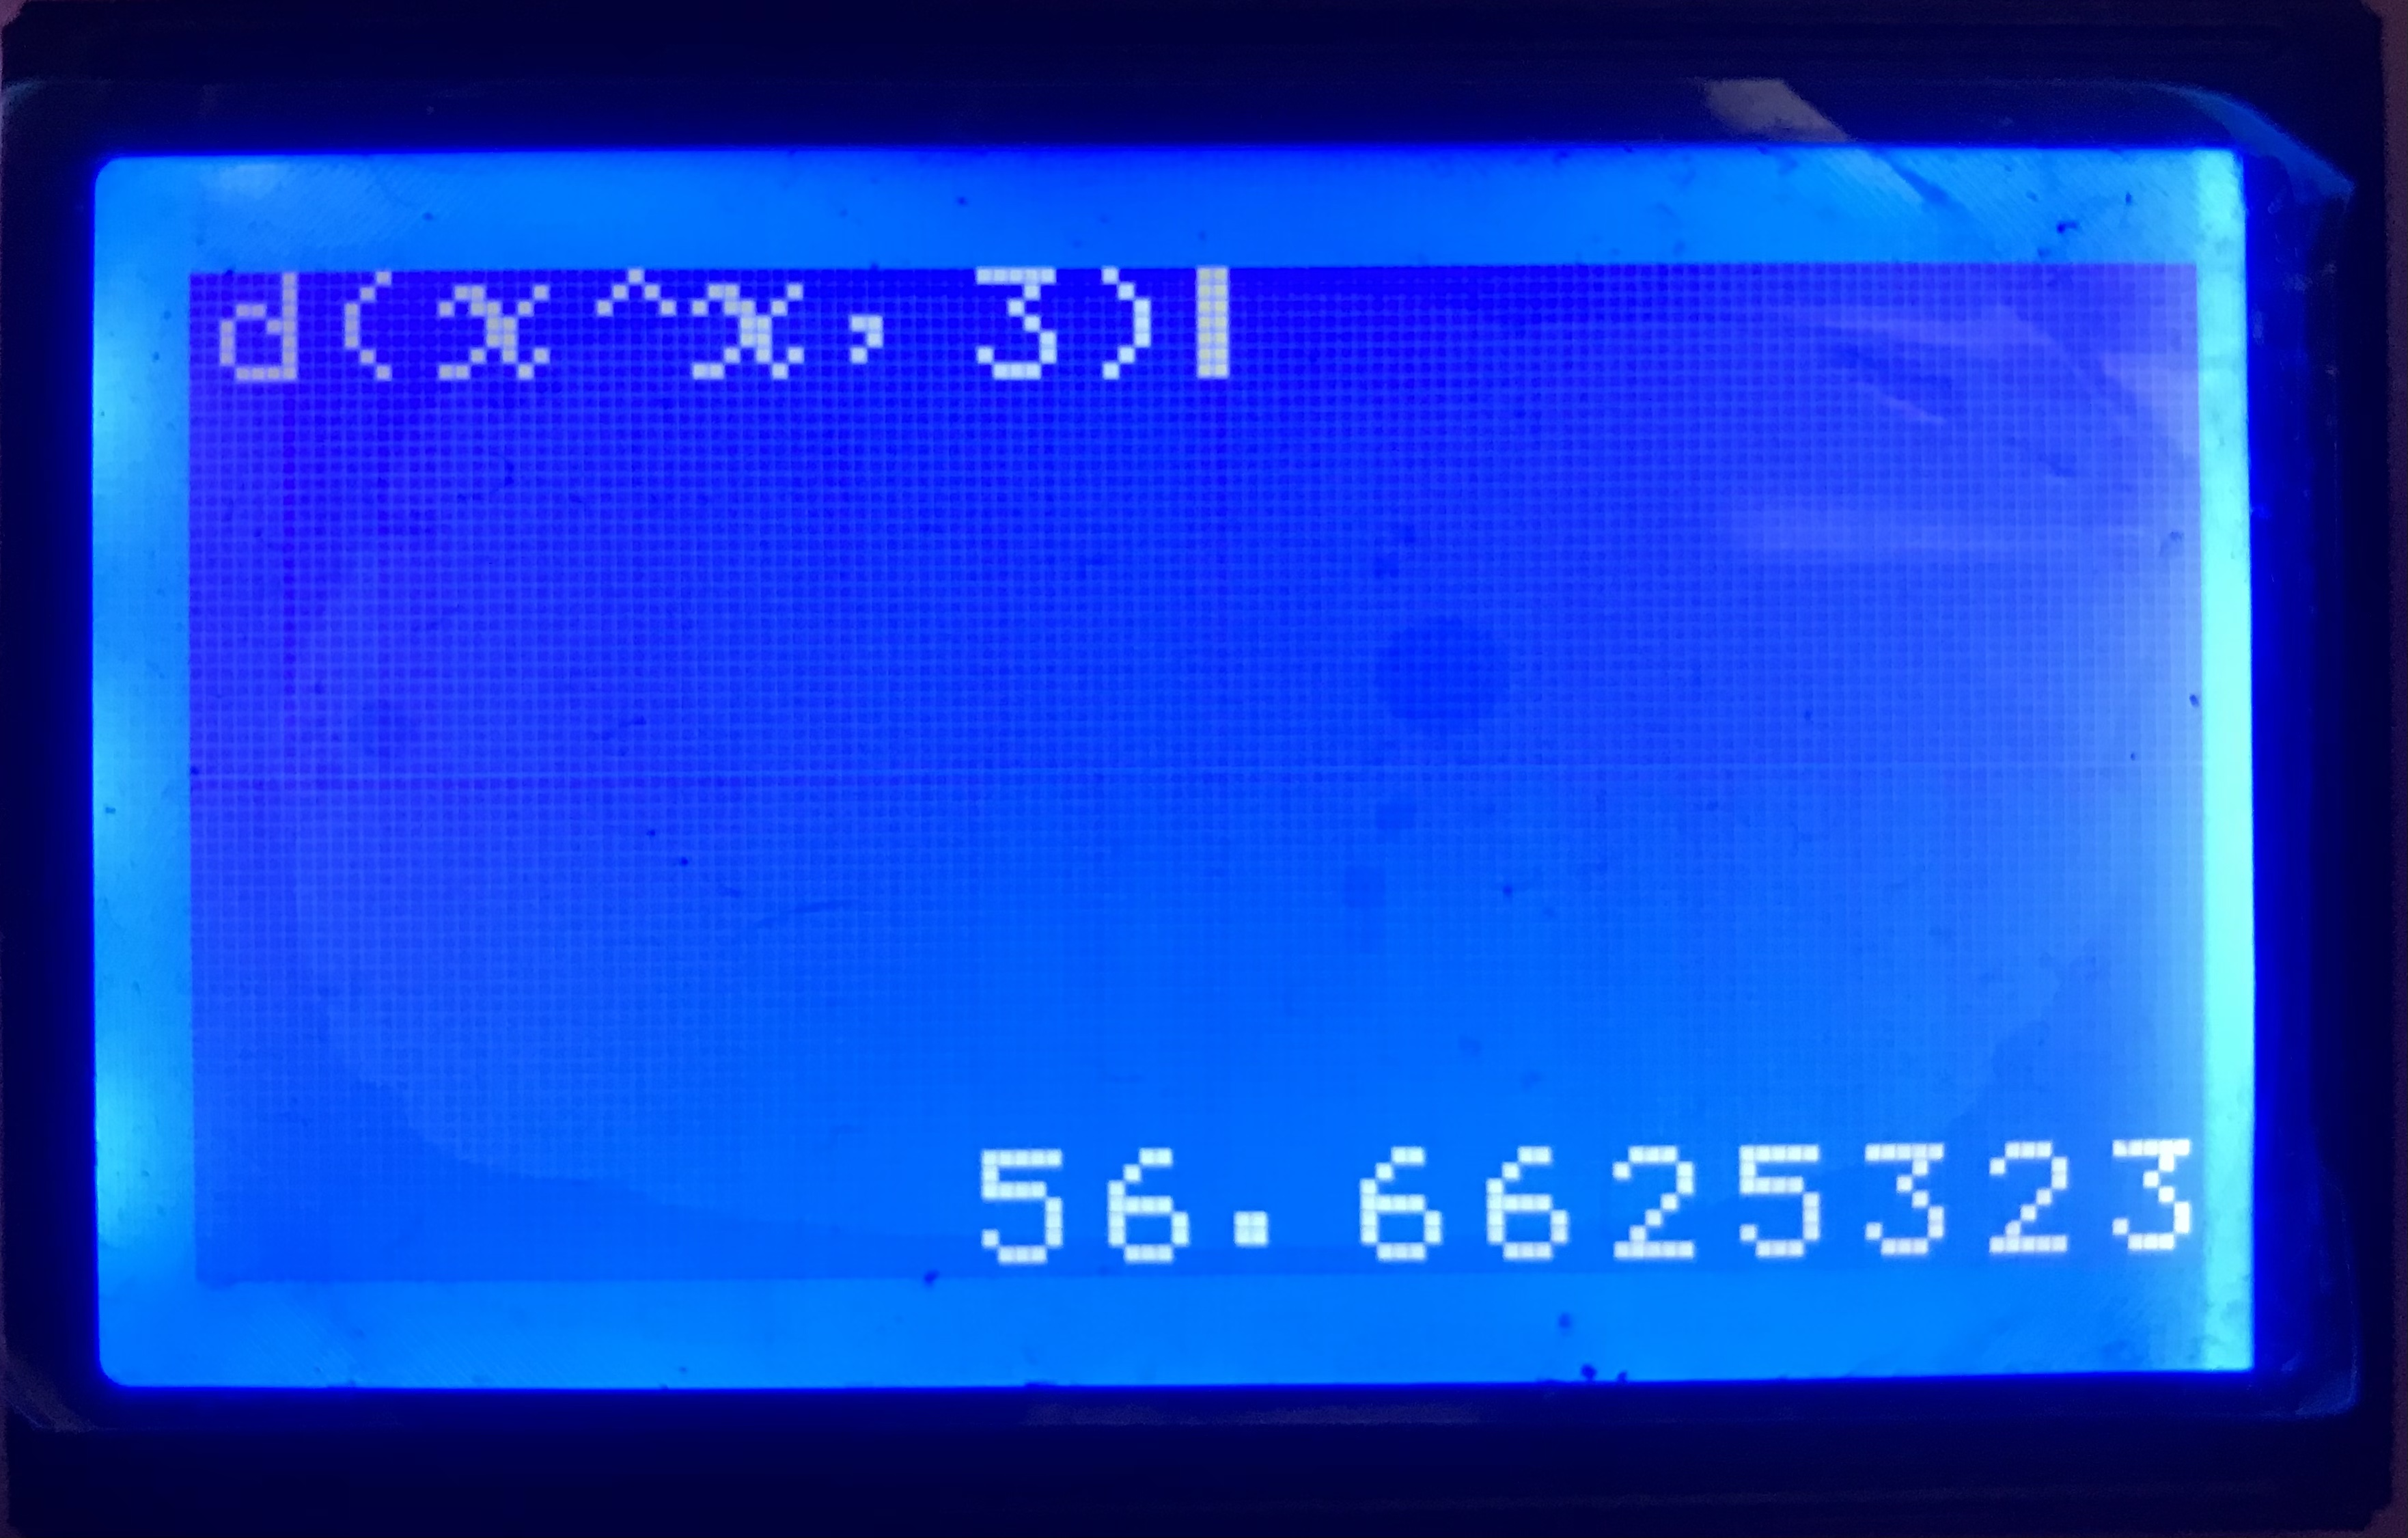
\includegraphics[width=.45\textwidth]{LCDScreens/der.jpeg}}
    
    \subfloat[][Evaluate $\int_1^{10}\ln xdx$ in UART mode]{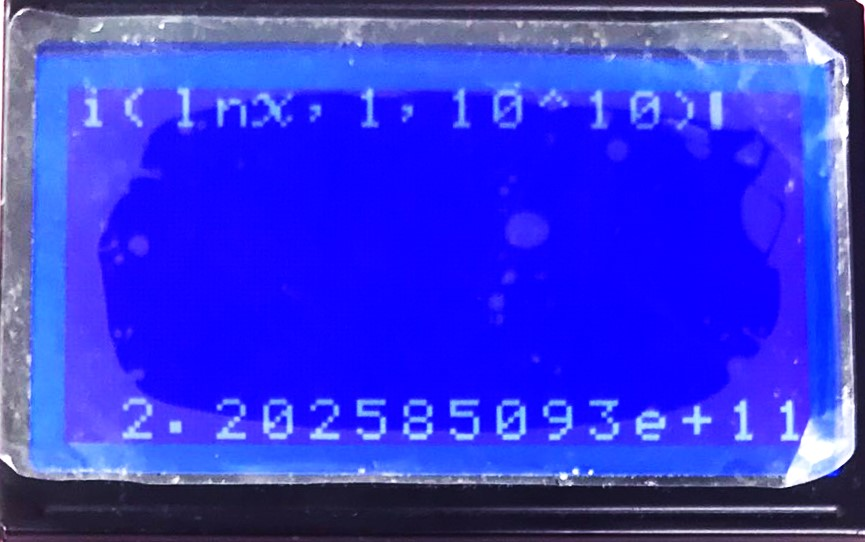
\includegraphics[width=.45\textwidth]{LCDScreens/calc_uart.jpg}}\quad
    \subfloat[][Evaluate $\int_1^{10}\ln xdx$ in UART mode (PC side)]{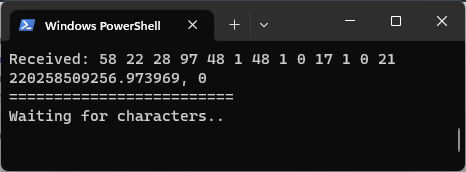
\includegraphics[width=.45\textwidth]{LCDScreens/calc_pc.png}}
    \caption{Math mode}
\end{figure}

\begin{figure}[H]
    \centering
    \subfloat[][]{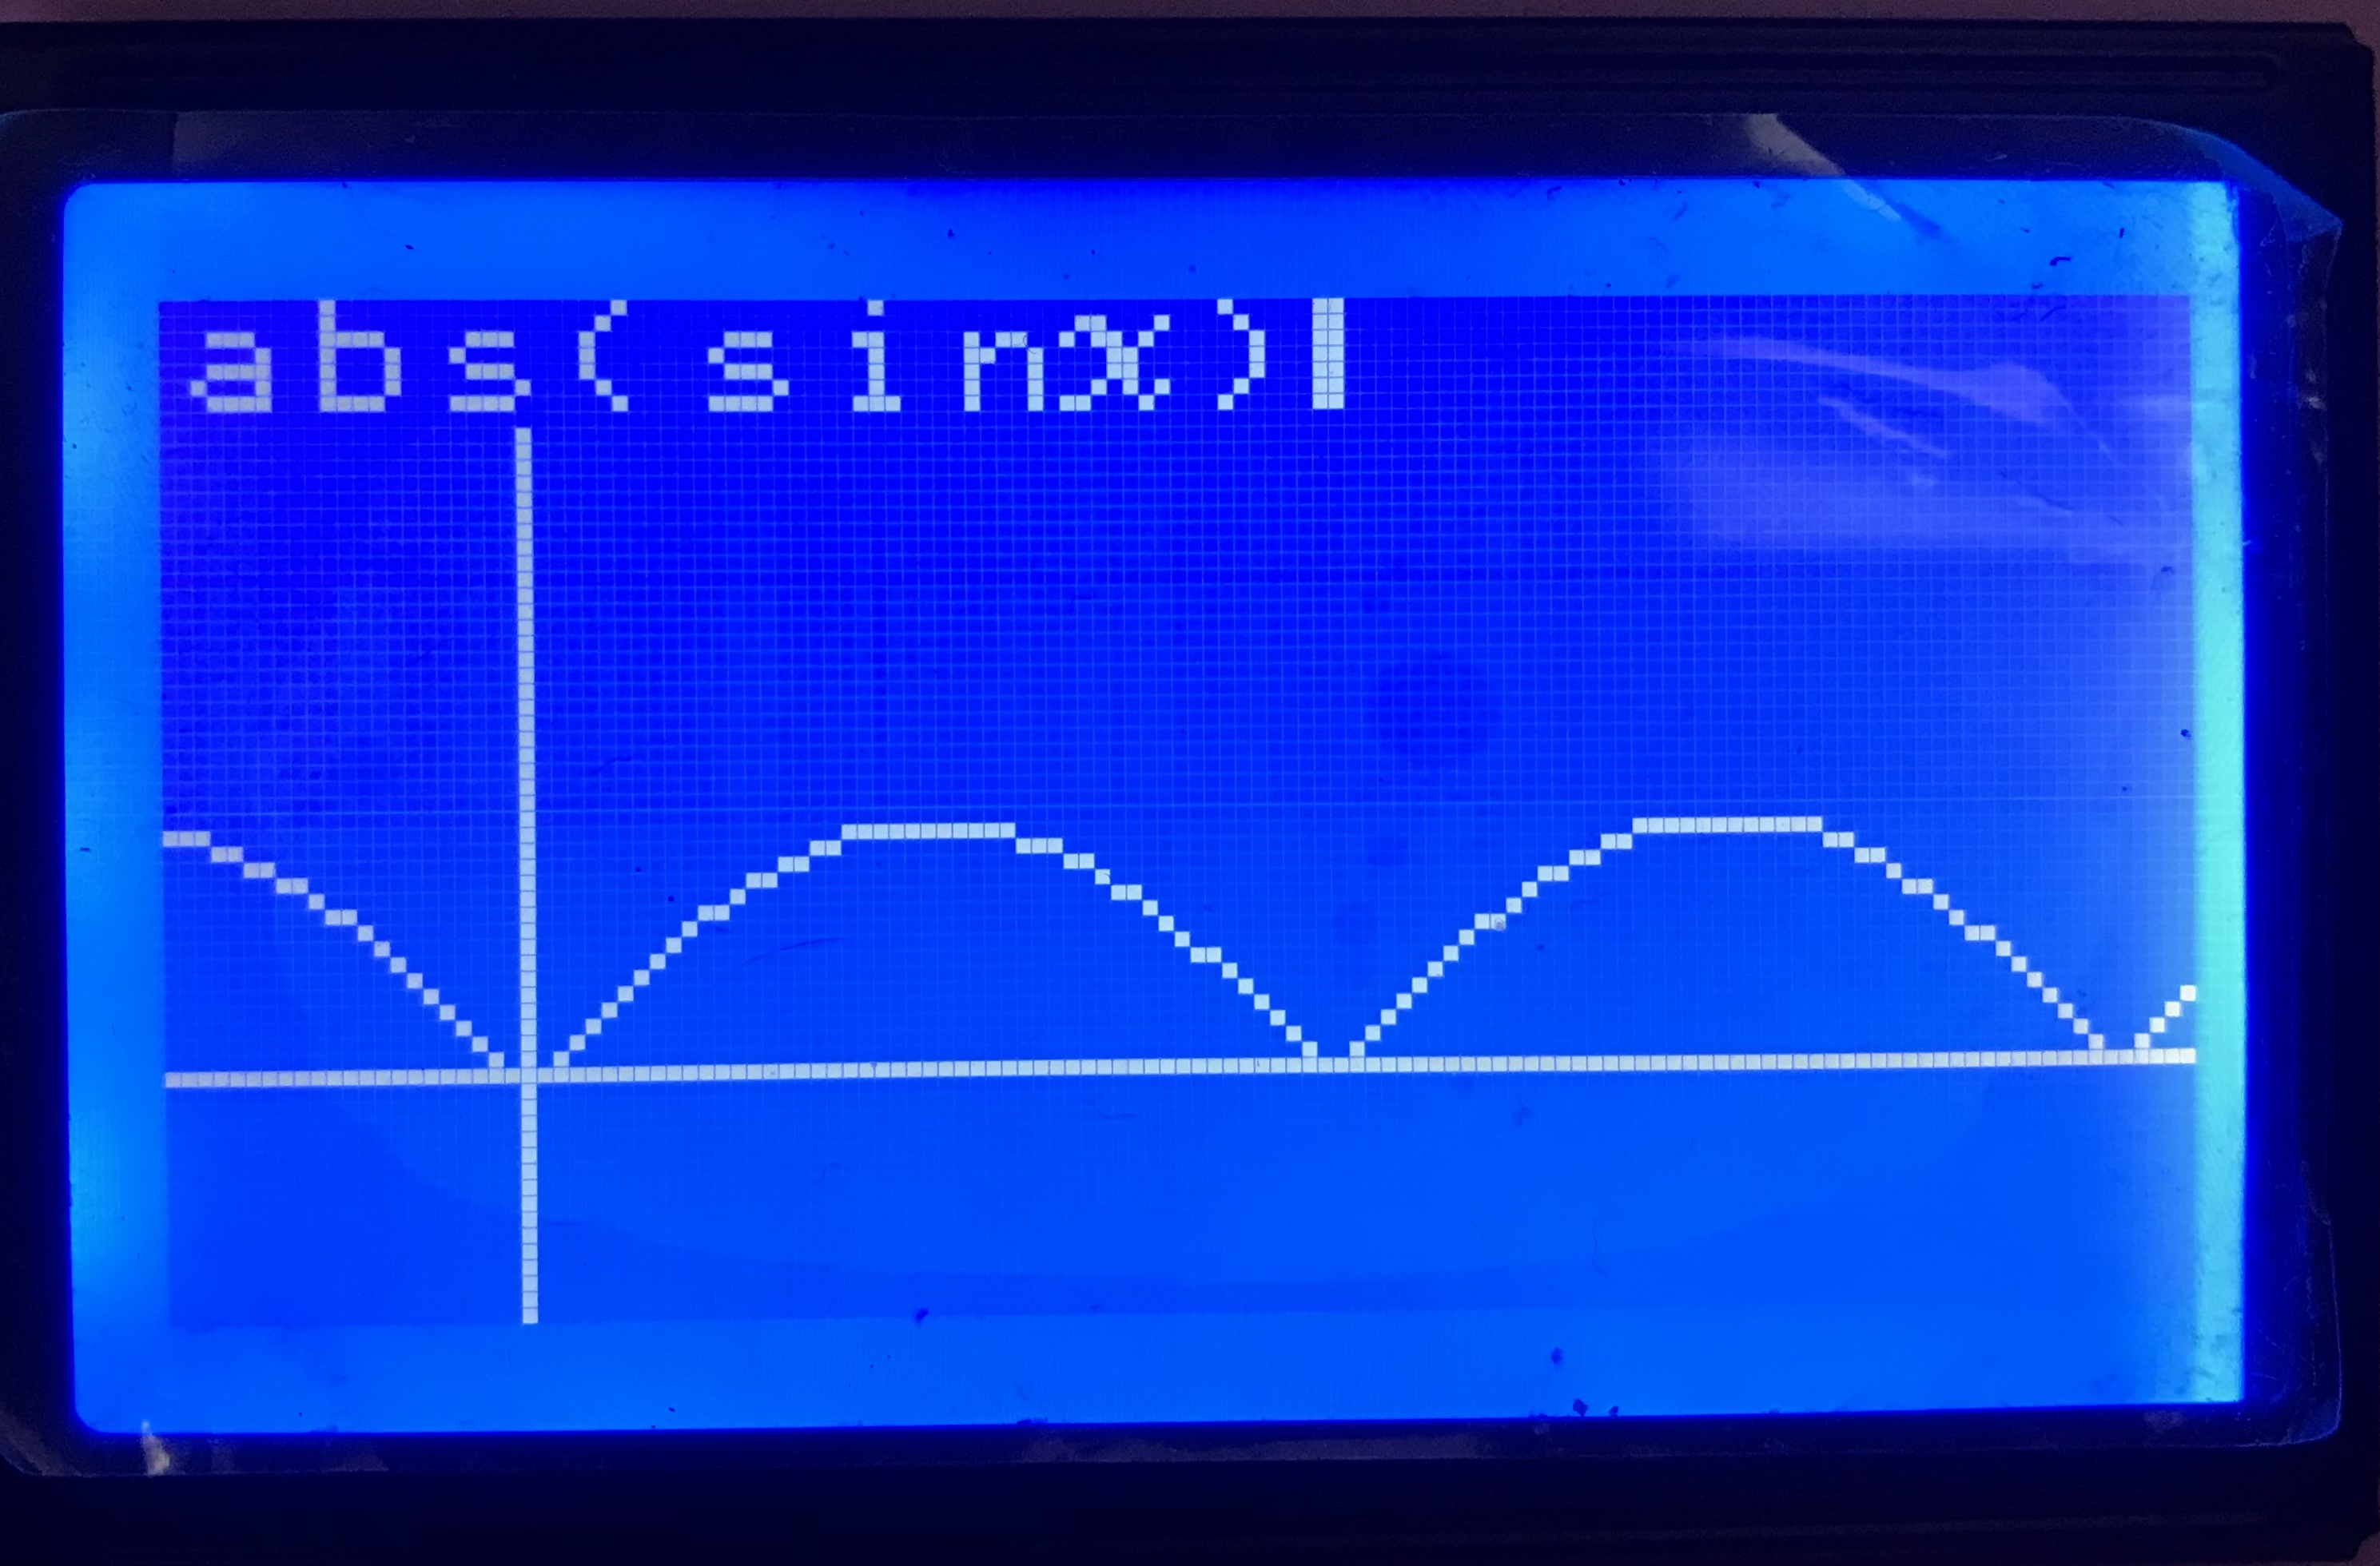
\includegraphics[width=.45\textwidth]{LCDScreens/graph.jpeg}}\quad
    \subfloat[][]{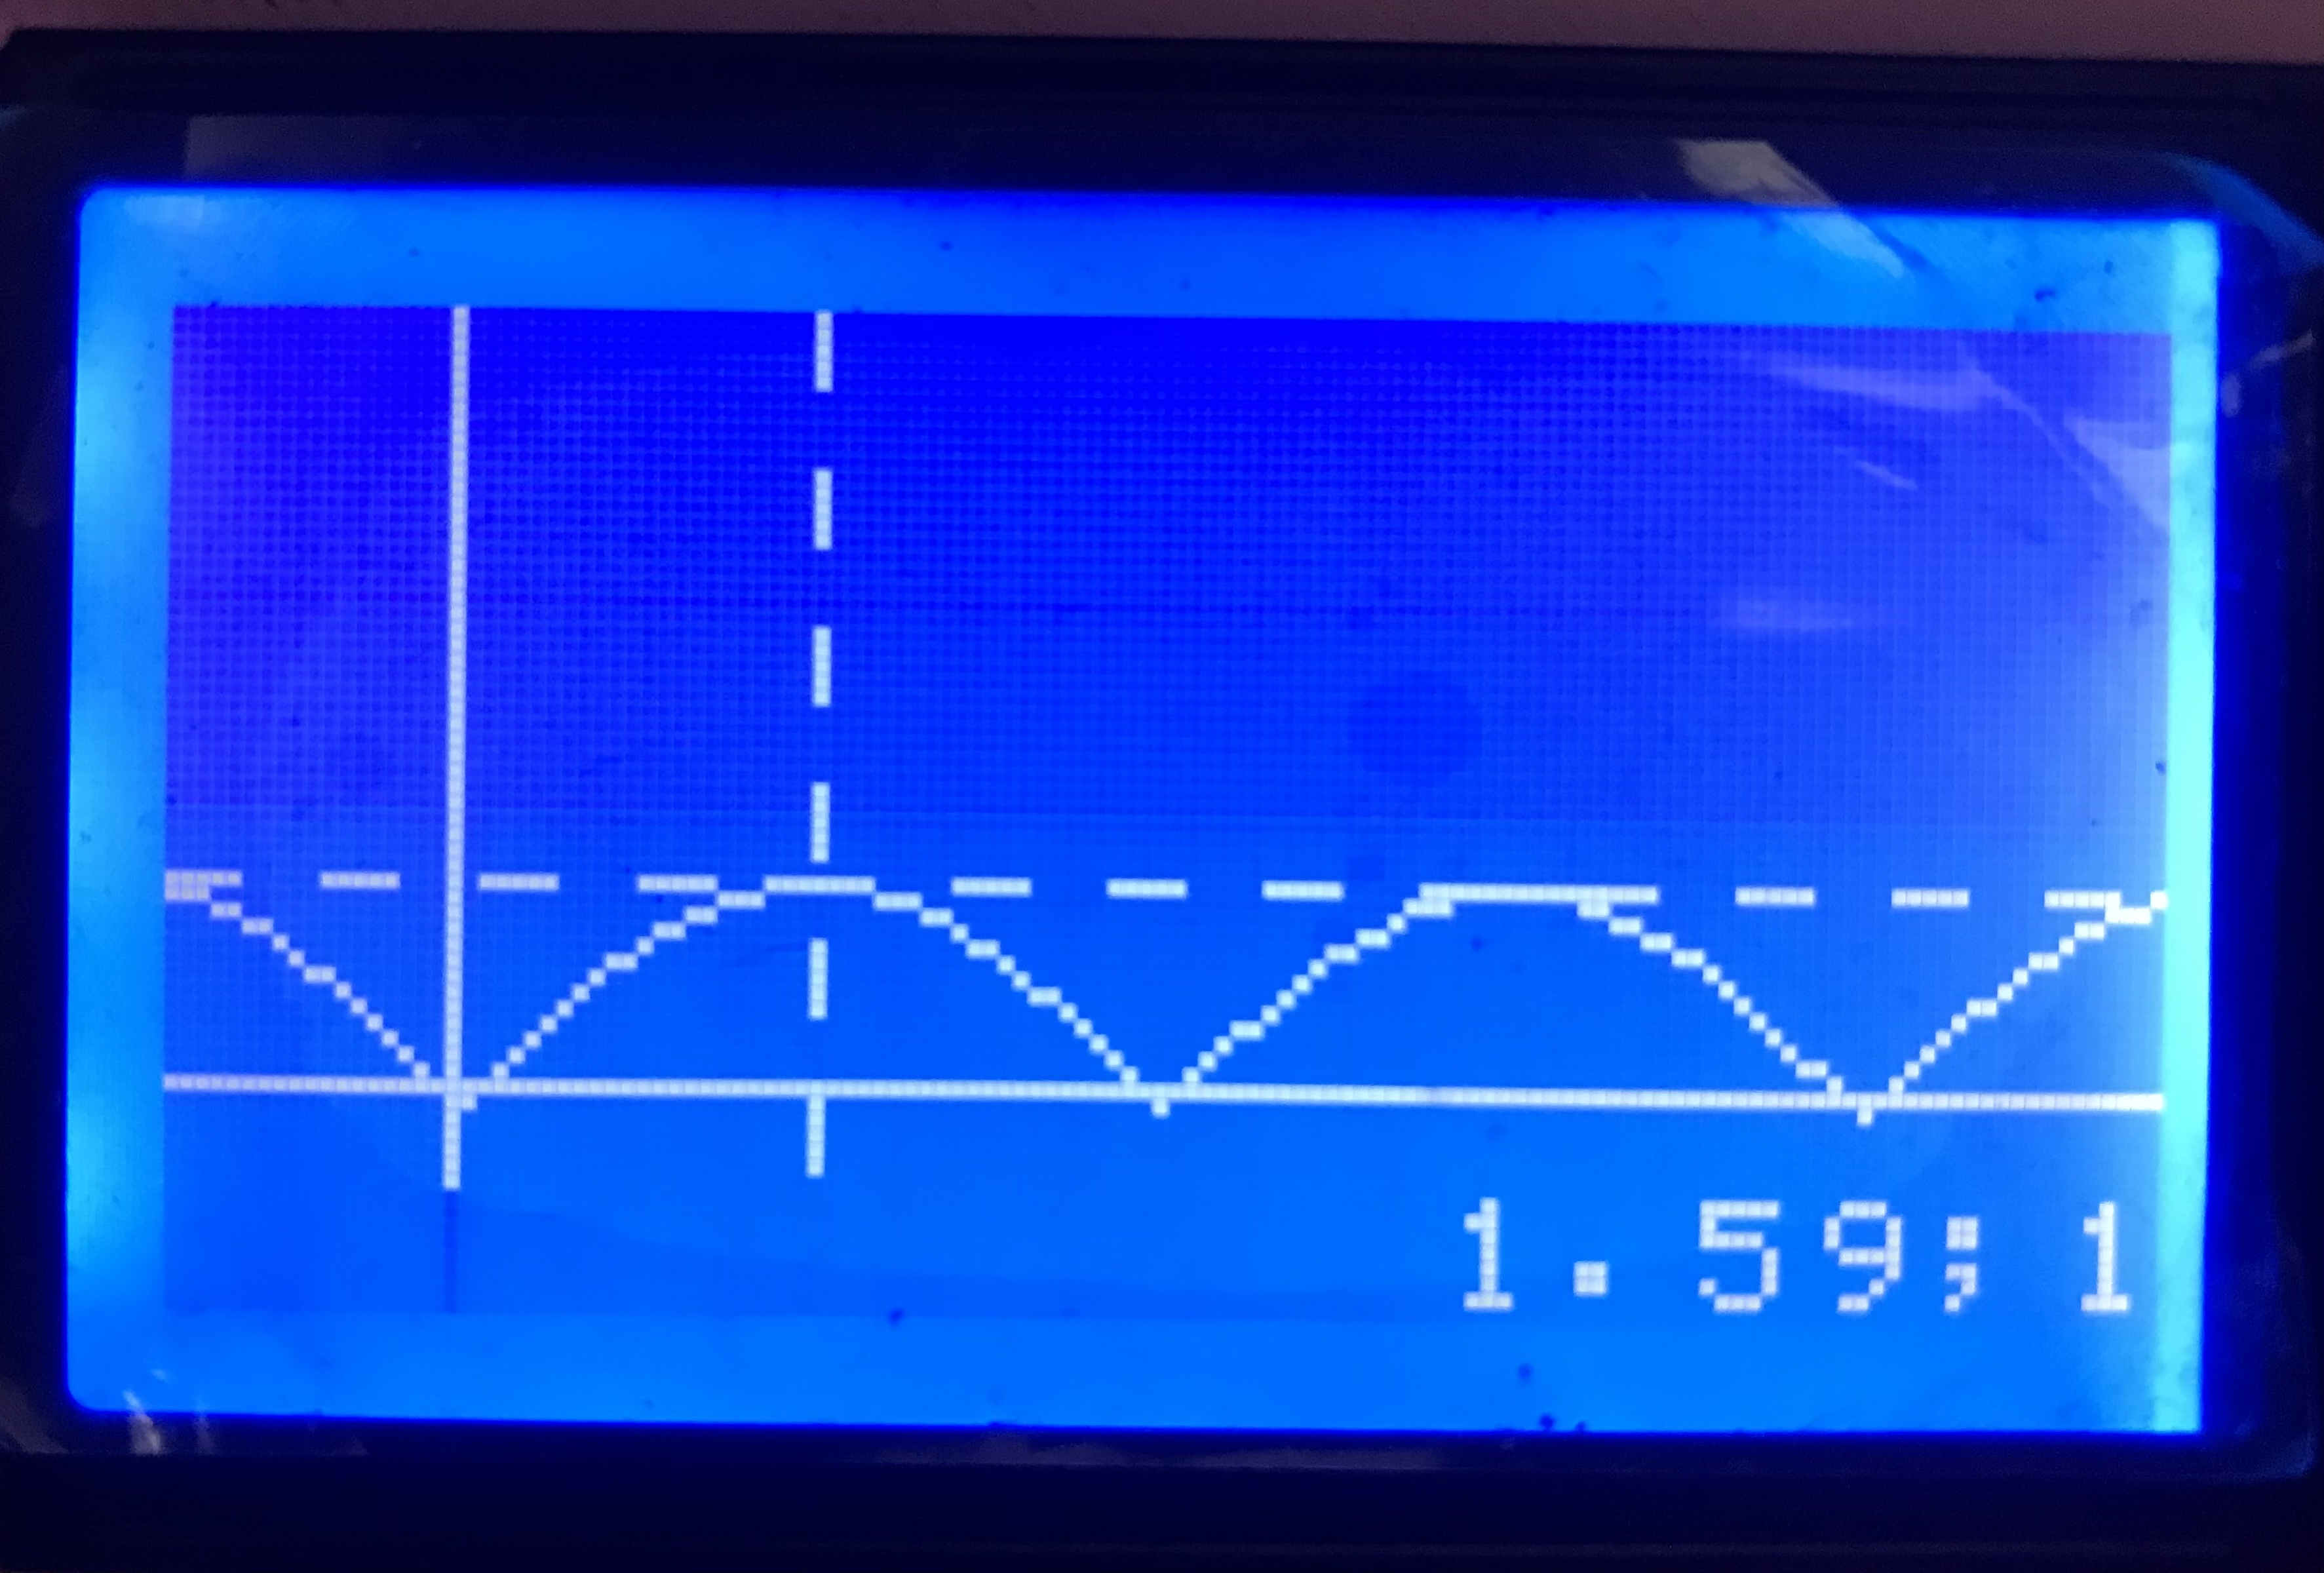
\includegraphics[width=.45\textwidth]{LCDScreens/graph_coord.jpeg}}
    \caption{Graphing $|\sin x|$}
\end{figure}

\chapter{Conclusion}
In conclusion, this project has been highly successful, with significant achievements in both hardware and software development. We have met half of the Functional and Non-functional requirements, completing 100\% of the assigned hardware tasks. This includes the meticulous design and successful implementation of the PCB, accompanied by a well-designed 3D-printed case that ensures optimal protection for all components. The integration of SWD and UART headers in the case enables convenient programming and communication capabilities. Overall, our team has demonstrated expertise in hardware design and fabrication, resulting in a robust and functional system.

In software development, we have achieved significant progress, completing around 50\% of the assigned tasks. Our focus has been on creating a comprehensive scientific calculator to cater to users' mathematical needs. The software supports fundamental arithmetic operations and advanced mathematical functions, including exponentiation, logarithms, trigonometric functions, and calculus operations like limits, derivatives, and integrals. The addition of graphing capabilities allows users to visualize functions and gain insights. To enhance usability, we have implemented a screen brightness adjustment feature for optimal visibility in various lighting conditions.

Throughout this project, our team has demonstrated exceptional dedication, creativity, and technical prowess. We have successfully brought together hardware and software components to create a functional and innovative calculator. The collaborative effort and effective project management have contributed to the project's overall success. We are proud of our accomplishments thus far and are excited about the potential for further development and refinement in the future. By continuing to enhance the calculator's capabilities and usability, we aim to provide users with a powerful tool for their mathematical endeavors.

Looking ahead, our future plans for the calculator project involve expanding its functionality and optimizing its design. We intend to incorporate specialized mathematical operations for engineering, physics, and finance, catering to specific fields. To achieve a sleek and compact design, we will focus on making the PCB smaller and replacing tactile buttons with a membrane keypad, reducing space and noise. Firmware upgrades will introduce advanced features like matrix computation, base changer, and additional constants. Furthermore, we aim to enhance the user experience by integrating a color screen, making the calculator more engaging and user-friendly.

\setcounter{biburllcpenalty}{7000}
\setcounter{biburlucpenalty}{8000}

\chapter{References}
\nocite{*}
\begin{otherlanguage}{vietnamese}
\AtNextBibliography{\large}
\printbibliography[heading=none]
\end{otherlanguage}

\vspace{2cm}
{\let\clearpage\relax \chapter*{Appendix}}
The project STM32 source code, Kicad PCB files and Autodesk Fusion 360 3D design will be available on our Github repository. Link: \url{https://github.com/superzeldalink/STM32-Scientific-Calculator}

\end{document}